% Change to 'masters' to produces the masters thesis preliminary pages
\documentclass[oneside,bachelor,etd]{WSUclass}

\usepackage{import}
% preamble contains title page, signature page, acknowledgment and abstract texts
\usepackage{preamble}
% Packages used
\usepackage[utf8]{inputenc} % Remove warning on ascii conversion
\usepackage[T1]{fontenc} % Remove warning on ascii conversion
\usepackage[backend=biber,refsection=part,style=nature,natbib=true]{biblatex}
\usepackage{bookmark}
%\usepackage{hyperref}
%\hypersetup{colorlinks=true,citecolor=blue}
\usepackage[pass]{geometry}
% \usepackage{showframe}
\usepackage{layout,layouts}
\usepackage{caption,subcaption}
\usepackage{pdflscape}
\usepackage{multicol,multirow}
\usepackage{newfloat}
\usepackage[newfloat=true]{minted}
\usepackage{physics,chemformula}
\usepackage{mathtools,nicefrac}
\usepackage{xcolor}
\usepackage{bm}
\usepackage{booktabs}
\usepackage{array,tabulary}
\usepackage{threeparttable}

% custom environment settings
\newcolumntype{K}[1]{>{\centering\arraybackslash}p{#1}}
\newenvironment{code}{\captionsetup{type=listing}}{}
\SetupFloatingEnvironment{listing}{name=Code}
\SetupFloatingEnvironment{listing}{placement=htpb!}

% Make chapter numbers into string words 1 -> ONE
\usepackage{fmtcount}
\makeatletter
\renewcommand{\@makechapterhead}[1]{\vspace *{40\p@ }{\parindent \z@ 
\raggedright \normalfont \ifnum \c@secnumdepth >\m@ne \Huge \bfseries 
\@chapapp \space \Numberstring{chapter} \vskip 10\p@ \fi #1\par \nobreak \vskip 30\p@ }}
\makeatother

\addbibresource{thesis.bib}

\begin{document}

\hypersetup{breaklinks=true}

% Start page counting in roman numerals
\frontmatter

% This command makes the formal preliminary pages.
% You can comment it out during the drafting process if you want to save paper.
\makepreliminarypages

\doublespace
% Make the table of contents.
\tableofcontents
\thispagestyle{plain}

% Make the list of tables
\mylistoftables
\thispagestyle{plain}

% Make the list of figures
\mylistoffigures
\thispagestyle{plain}

% This page is OPTIONAL. To remove, comment out and \dedicationpage in diss.tex
%  \dedicationpage
\clearemptydoublepage

% Start regular page counting at page 1
\mainmatter

% OK. Everything is set up. Type your thesis here.

\currentpdfbookmark{CHAPTER}{CHAPTER}

\addchapheadtotoc


\chapter{Introduction}
Density Functional Theory proved to be useful and reasonably accurate in determining the physical nature of defects in semiconductors, including  but not limited to native defects, impurities, dopants, and surface defects. 

\section{Purpose and Motivation}
Describe the importance of defects in ZnO
\section{Objectives}
\begin{itemize}
    \item to obtain the bandstructure and density of states of native point defects in wurtzite \ch{ZnO}
    \item to determine which atomic orbitals  contribute to the defect energy level
\end{itemize}

This study considers only the native point defects in ZnO: oxygen and zinc vacancies (\ch{V_O} and \ch{V_{Zn}}), interstitials (\ch{O_i} and \ch{Zn_i}), antisites (\ch{O_{Zn}} and \ch{Zn_O}) and charged defects (\ch{V_O^{1+}}, \ch{V_O^{2+}}, \ch{Zn_i^{1+}} and \ch{Zn_i^{2+}}). 
% Study the mechanisms of different defects in ZnO
\section{Outline}

% \chapter{Acronym Used}

\chapter{Review of Related Literature} \label{chap:rrl}
% \section{Semiconductors}
%     \subsection{Properties}
%     \subsection{Applications of Semiconductors}
%     \subsection{Defects in Semiconductors}
\section{Properties of ZnO}
% \section{Zinc Oxide}
	describe ZnO in broad perspective
	donors and acceptors
	excitation in semiconductors
\section{Crystal Structure}
There are three possible crystal structures (phases) of \ch{ZnO}, namely: wurtzite, zinc blende, and rocksalt. The wurtzite structure belongs to the space group $C^4_{6v}$ in Schoenflies notation, $P6_3mc$ in the  Hermann–Mauguin notation, and space group number 186 in International Tables for Crystallography (ITA) notation \citep{Hahn2005}. The crystal structure of wurtzite ZnO is shown in Figure \ref{fig:ZnO_unit}. Each zinc atom is surrounded by four oxygen atoms, which are located
at the corners of an irregular tetrahedron.

\begin{figure}[tbh!] 
	\centering
	\includegraphics[width=0.5\linewidth]{"images/rrl/ZnO_unit"}
	\caption[Crystal structure of wurtzite \ch{ZnO} unit cell]{Crystal structure of wurtzite \ch{ZnO} unit cell}
	\label{fig:ZnO_unit}
\end{figure}

\section{Brillouin Zone Symmetry}
	The primitive vectors of the direct (real) hexagonal lattice are 
\begin{align}
	\va{a}_1 &= a \vu*{x}	\\
	\va{a}_2 &= \frac{a}{2} \vu*{x} + \frac{\sqrt{3}a}{2} \vu*{y} \\
	\va{a}_3 &= c \vu*{z}
\end{align}
where $a$ and $c$ are the lattice parameters of hexagonal \ch{ZnO}. On the other hand, the primitive vectors of the reciprocal lattice can be derived using the formula \eqref{eq:recipro_real} in Appendix \ref{chap:BZ} 

\begin{align}
	\va{b}_1 &= \frac{2 \pi}{a} \left(\vu*{k}_x - \frac{1}{\sqrt{3}} \vu*{k}_y \right) \\ 
	\va{b}_2 &= \frac{2 \pi}{a} \left( \frac{2}{\sqrt{3}} \vu*{k}_y \right) \\
	\va{b}_3 &= \frac{2 \pi}{a} \left( \frac{a}{c} \vu*{k}_z  \right)
\end{align}

The first Brillouin Zone of an hexagonal lattice is also an hexagonal. For more details about reciprocal lattice and Brillouin zones, see Appendix \ref{chap:BZ}.  Figure \ref{fig:HS} shows the symmetry points inside the first Brillouin zone. The capital letters represent the high symmetry (HS) points inside the first Brillouin zone where their notations were traditionally used in the solid state physics literature \citep{Bouckaert1936}. Their  values are shown in Table \refeq{tab:HS}.  The different symmetry points of wavevectors correspond to the different kinds of irreducible representations of the space group \citep{Shmueli2001,Aroyo2006,PerezMato2011,Aroyo2014}. 

\begin{figure}[tbh!] 
	\centering
	\includegraphics[width=0.48\linewidth]{"images/rrl/hex"}
	\caption[The first Brillouin zone of a typical hexagonal Bravais lattice]{The first Brillouin zone of a typical hexagonal Bravais lattice. Figure taken from \citep{Setyawan2010}.}
	\label{fig:HS}
\end{figure}


\begin{table}[tbh!]
	\centering
	\caption{High symmetry points of an hexagonal Bravais lattice}
	\label{tab:HS}
	\begin{tabular}[t]{K{0.15\linewidth}K{0.1\linewidth}K{0.1\linewidth}K{0.1\linewidth}}
	\toprule
	\textbf{HS} & $\times \va{b}_1$ & $\times \va{b}_2$ & $\times \va{b}_3$ \\ \midrule
	$\Gamma$ & 0 & 0 & 0 \\
	$A$ & 0 & 0 & 1/2 \\
	$H$ & 1/3 & 1/3 & 1/2 \\
	$K$ & 1/3 & 1/3 & 0 \\
	$L$ & 1/2 & 0 & 1/2 \\
	$M$ & 1/2 & 0 & 0 \\ \bottomrule
	\end{tabular}
\end{table}

\clearpage


% \section{Crystallographic Directions and Planes}
text
\section{Photoluminescence Properties}
ZnO often exhibits green luminescence which has a peak around 2.4 and 2.5 eV.
\section{Defects}
add Kröger-Vink Notation for defects

consider degenerate semiconductors?

 
\chapter{Theoretical Framework}
\section{Electronic Structure}
The problem of electronic structure methods begins with the attempt to solve the general non-relativistic time-independent Schr\"{o}dinger equation given as \citep{Schroedinger1926}
\begin{equation} \label{eq:schrodinger}
	\hat{\mathcal{H}} \Psi = E \Psi
\end{equation}
where $\hat{\mathcal{H}}$ is the Hamiltonian operator for a system of electrons, $\Psi$ is the electronic wavefunction and $E$ is the energy of the system. Consider a single electron in three dimensional system, the Schr\"{o}dinger equation can be expressed as
\begin{equation} \label{eq:1e_wave}
	\hat{\mathcal{H}} \Psi_n = - \frac{\hbar^2}{2m} \left(\pdv[2]{x} + \pdv[2]{y} + \pdv[2]{z} \right) \Psi_n + V \Psi_n  = \epsilon_n \Psi_n
\end{equation}
where $m$ is the mass of electron, $V$ is the effective potential energy and $\epsilon_n$ is the energy of electron in the orbital. The term orbital denotes the solution of the Schr\"{o}dinger equation for a system of only one electron. This will be useful in later sections because this will allow to distinguish between the exact quantum state of a system of $N$ interacting  electrons
from the approximate quantum state of $N$ electrons in $N$ orbitals, where each orbital is a solution to one-electron wavefunction in \eqref{eq:1e_wave}. If $V$ is zero for the case of free electrons (i.e. non-interacting), then the orbital model is exact.

Since electrons are restricted by the potential inside the atom, the simplest way of solving \eqref{eq:1e_wave} is by considering an infinite potential well. The electrons are confined inside a cube of length $L$ where the potential $V$ inside is zero and infinite at outside must satisfy the boundary condition

\begin{equation}
	\Psi_n(L_x,L_y,L_z) = 0
\end{equation}
where $L_x,L_y,L_z$ can be either 0 or $L$. The solution will have a sine dependence

\begin{equation}
	\Psi_n(x,y,z) = \sqrt{\left(\frac{2}{L}\right)^3} \ \sin(\frac{n_x \pi }{L} x) \sin(\frac{n_y \pi}{L} y) \sin(\frac{n_z \pi}{L} z)
\end{equation}
where $n_x,n_y,n_z$ are integer quantum states. Provided that $ k_i = n_i \pi / L$ where $i=x,y, \text{or}\, z$; then the energy dispersion relation can be expressed as
\begin{equation} \label{eq:free_e}
	\epsilon_k = \frac{\hbar^2}{2m} (k_x^2 + k_y^2 + k_z^2) = \frac{\hbar^2}{2m} k^2 \propto k^2
\end{equation}
Note that energy levels are discretized by the quantum states which arises from imposing the boundary conditions.
\subsection{Electronic Band structure} \label{sec:bands}
Inside the crystal lattice, the periodic arrangement of atoms or ions causes the potential to be periodic which eventually gives rise to the formation of energy bands. The wavefunction $\Psi$ will become periodic in space with a period $L$ and must obey the Born-von Karman boundary condition \citep{Herman1959}
\begin{equation} \label{eq:periodic}
	\Psi_k(x,y,z) = \Psi_k(x + L, y, z)
\end{equation}
and similarly for the $y$ and $z$ coordinates. It can be shown that wavefunctions satisfying \eqref{eq:1e_wave} and \eqref{eq:periodic} are the Bloch form of a travelling plane wave
\begin{equation} \label{eq:Bloch}
	\Psi_k(\va{r}) = u_k(\va{r}) \exp(i \va{k} \vdot \va{r})
\end{equation}
where $u_k(\va{r})$ has the period of the crystal lattice with $u_k(\va{r}) = u_k(\va{r} + \va{R})$. Here $\va{R}$ is the translation vector which can be simply thought as the periodicity expressed as vector.  The Bloch expression can be written as
\begin{align}
	\Psi_k(\va{r} + \va{R}) & = u_k(\va{r} + \va{R}) \exp(i \va{k} \vdot (\va{r} + \va{R}))  \notag         \\
	\Psi_k(\va{r} + \va{R}) & = u_k(\va{r}) \exp(i \va{k} \vdot \va{r})  \exp(i \va{k} \vdot \va{R}) \notag \\
	\Psi_k(\va{r} + \va{R}) & = \Psi_k(\va{r}) \exp(i \va{k} \vdot \va{R})
\end{align}

Notice that the wavefunction differs from the plane wave of free electrons only by a periodic modulation given by the new phase factor. This means that the electrons in the crystal lattice are treated as perturbed weakly by the periodic potential of the ion cores.

% in which the components of $\va{k}$ satisfy
% \begin{equation}
%     k_i = \pm \frac{2n_i \pi}{L} \quad ; i = x,y,z \quad; n_i = 0, 1, 2, \dots
% \end{equation}

\subsubsection{Band structure of free electron}
A special case of periodicity is where the potential is set to zero, which is applicable for the free electrons. The wavefunction will be a plane wave
\begin{equation}
	\Psi_k(\va{r})  = \exp(i \va{k} \vdot \va{r})
\end{equation}
that represents travelling wave with a momentum $\va{p} = \hbar \va{k}$. The energy dispersion relation is still given by \eqref{eq:free_e} but this time the allowed energy values are distributed essentially from zero to infinity. Figure \ref{fig:free-electron} shows the parabolic dependence of energy with the wavevector $k$. Since the system is periodic in real space, it must be true for the reciprocal space, in this case by $2\pi/a$ where $a$ is some lattice constant. Figure \ref{fig:free-electron}a shows the extended zone scheme where there are no restrictions on the values of wavevector $\va{k}$. When wavevectors are outside the first Brillouin zone (BZ), they can be translated back to the first zone by subtracting a suitable reciprocal lattice vector. In mathematical sense \citep{Kittel2004}
\begin{equation} \label{eq:band_fold}
	\va{k} + \va{G} = \va{k'}
\end{equation}
where $\va{k'}$ is the unrestricted wavevector, $\va{k}$ is in the first Brillouin zone, and $\va{G}$ is the translational reciprocal lattice vector. The energy dispersion relation can always be written as
\begin{align}
	\epsilon(k_x,k_y,k_z) & = \frac{\hbar^2}{2m} (\va{k}+\va{G})^2 \notag                       \\
	                      & = \frac{\hbar^2}{2m}[(k_x + G_x)^2 + (k_y + G_y)^2 + (k_z + G_z)^2]
\end{align}
Figure \ref{fig:free-electron}b shows the reduced zone scheme where the  bands are folded into the first BZ by applying \eqref{eq:band_fold}. Any energy state beyond the first BZ is the same to a state inside the first BZ with a different band index $n$.

\begin{figure}[tbh!]
	\centering
	\includegraphics[width=0.6\linewidth]{"images/theory/bands_free"}
	\caption[Free electron band structure]{Free electron band structure where (a) is in the extended zone scheme and (b) in the reduced zone scheme. The dotted lines in (a) lies the first BZ.}
	\label{fig:free-electron}
\end{figure}

\subsubsection{Band structure of electrons in solids}
When atoms are very far from each other with no interaction, each electron occupies specific discrete orbitals such as 1s, 2p, 3d, etc. When they are bring  closer enough, the outermost (valence) electrons interact with each other and will result in the  energy level splitting. The innermost (core) electrons remain as they are, since they are closer to the nuclei and bounded by a deep potential well. For a solid containing a large $N$ atoms, there will be $N$ orbitals (i.e. $N$ 3d-orbitals) trying to occupy the same energy level. Pauli's exclusion principle will prevent this from happening, hence what happens is there will be splitting of the energy level that are closely spaced and this will eventually form a continuous band of energy levels. Figure \ref{fig:band_model} summarizes the evolution of energy levels as the atoms are brought together.

\begin{figure}[tbh!]
	\centering
	\includegraphics[width=0.7\linewidth]{"images/band model"}
	\caption[Band structure in solids]{Formation of bands and band gaps when isolated atoms are bring closer together. Figure taken from \citep{Lee2016}}
	\label{fig:band_model}
\end{figure}

Another interesting property of band structure is the formation of energy band gaps. This happens when the valence electrons interact with the periodic potential of the nuclei. Assuming a weak periodic potential, most of the band structure will not changed very much, except possibly at the Brillouin zone boundaries with a wavevector of $\va{k} = n \pi/ a$. The orbitals with the wavevector at zone boundaries, chosen to be at high symmetry points, follows the Bragg diffraction condition and thus are diffracted. The valence electrons are scattered (or reflected) at the zone boundary in which the wavefunction are made up of equal plane waves travelling from the left and from the right. The wavefunction becomes a standing wave that resembles more of those bound states. Hence, there will be a forbidden region where travelling waves are not allowed. If sufficient energy is provided to the electron, they can overcome the  binding potential.

The band gap is generally referred to the energy difference between the top of valence band, Valence band maximum (VBM),  and the bottom of the conduction band, Conduction band minimum (CBM). If VBM and CBM coincides with each other, the material is said to be a conductor. Electrons can easily occupy the conduction band without any excitation, hence electrons are highly mobile that will lead to high current. For band gaps with a value comparable to the quantity $k_B T$, where $k_B$ is the Boltzmann constant and  $T$ is the absolute temperature near room temperature, then the material is semiconductor. If band gap is much larger than $k_B T$, then the material is insulator. However, this criterion is very loose because there are materials with large band gaps such as \ch{ZnO}, \ch{SrIn2O4}, and diamond that are categorized as semiconductors. These materials are generally called wide-band gap semiconductors. If the VBM and CBM are located in the same wavevector $k$, then the gap is direct. Otherwise, it is indirect.

\subsection{Density of States}
Another useful quantity in describing the electronic structure is the density of states (DOS). In general, the density of states can be defined as \citep{Ashcroft1976}
\begin{equation} \label{eq:dos_sum}
	D(\epsilon) = 2 \sum_n \sum_k \delta(\epsilon - \epsilon_n(k))
\end{equation}
where for each band index $n$, the sum is over all allowed values of $k$ lying inside the first Brillouin zone. The factor 2 comes from the allowed values of the spin quantum number for each allowed value of $k$. In the limit of large crystal, the $k$ points are very close together, and the sum can be replaced by an integral. Since each allowed states will take up a volume of $ (\Delta k)^3 = \pi^3/V$ where $V$ is the volume of the solid in real space, it is convenient to write \eqref{eq:dos_sum} as
\begin{equation} \label{eq:dos_int}
	D(\epsilon) = 2\, \frac{V}{\pi^3} \sum_n \sum_k \delta(\epsilon - \epsilon_n(k)) (\Delta k)^3
\end{equation}
for  in the limit of $V \rightarrow \infty $, $\Delta k \rightarrow 0$, it becomes

\begin{equation}
	\lim_{V \to \infty} \frac{1}{V}\, D(\epsilon) = \frac{2}{\pi^3} \sum_n \int \delta(\epsilon - \epsilon_n(k)) \dd[3]{k}
\end{equation}
Usually, the total DOS is set to be the number of states per unit energy per unit volume.

The DOS can be projected in terms of the orbital contribution of each atoms. This can be expanded in a complete orthonormal basis as \citep{Enkovaara2010}

\begin{align}
	D(\epsilon) & = \sum_i D_i(\epsilon)                                                                            \\
	            & = \sum_i \sum_n \int \bra{\psi_n} \alpha \ket{\psi_n}  \delta(\epsilon - \epsilon_n(k)) \dd[3]{k}
\end{align}
where $D_i(\epsilon)$ is the projected density of states (PDOS) of orbital $i$ with state $\alpha$.

\section{Many-body Physics}
Despite the simplicity of Schr\"{o}dinger equation in \eqref{eq:schrodinger}, solving it is a formidable task when dealing with many-electron systems. Analytical solutions to this equation only exist for the very simplest systems (i.e. hydrogenic atoms). Solving beyond '2 particle' system (electron and nucleus) is already intractable. In addition, solid state systems typically contains more than hundreds of particles, resulting in hundreds of simultaneous equations. Even the use of computational methods relies on a number of approximations just to make computations feasible enough. Hence, this section will discuss various levels of approximations without neglecting the parameter-free of first-principles calculations.

\subsection{Many-particle Hamiltonian Operator}
The exact many-particle Hamiltonian is consist of five operators which can be expressed as
\begin{equation}
	\hat{\mathcal{H}} = \hat{\mathcal{T}_n} + \hat{\mathcal{T}_e} + \hat{\mathcal{V}}_{en} + \hat{\mathcal{V}}_{ee}  + \hat{\mathcal{V}}_{nn}
\end{equation}
where the $\hat{\mathcal{T}}$ and $\hat{\mathcal{V}}$ refer to kinetic energy and potential energy, respectively, and the labels $e$ and $n$ denotes the electronic and nuclear coordinates and their derivatives, respectively.  This equation can be expanded as
\begin{multline} \label{eq:many_se}
	\hat{\mathcal{H}}  = - \frac{\hbar^2}{2} \sum_I \frac{\laplacian_{\va*{R_I}}}{M_I} - \frac{\hbar^2}{2} \sum_i \frac{\laplacian_{\va*{r_i}}}{m_e} \\
	- \frac{1}{4 \pi \epsilon_0} \sum_{I,i} \frac{e^2 Z_I}{\abs{\va*{R_I} - \va*{r_i}}} + \frac{1}{8 \pi \epsilon_0} \sum_{i\neq j} \frac{e^2}{\abs{\va*{r_i} - \va*{r_j}}} + \frac{1}{8 \pi \epsilon_0} \sum_{I\neq J} \frac{e^2 Z_I Z_J}{\abs{\va*{R_I} - \va*{R_J}}}
\end{multline}
where $M_I$ is the mass of the $I$th nuclei (or usually ions) with charge $Z_I$ located at site $\va*{R_I}$, and electrons have mass $m_e$  located at site $\va*{r_i}$. The first and second terms are the kinetic energy of the atomic nuclei and electrons, respectively. The last three terms
describe the Coulomb interaction between electrons and nuclei, between electrons and other electrons, and between nuclei and other nuclei.

\subsection{Simplifying Assumptions}
Solving \eqref{eq:many_se} exactly is very impractical and not worth the effort. Hence, we resort to approximations in order to find acceptable eigenstates.

The first level of approximation is the Born-Oppenheimer approximation or the Adiabatic approximation \citep{Born1927}. It begins with the observation that the mass of nuclei is much larger compared to the electron, as such one can assume that electrons moving in a potential much faster than the nuclei and that the nuclei can be treated as fixed or 'frozen' with respect to motion. As a consequence, the nuclear kinetic energy will be zero and the nuclear interaction with the electron cloud  can be treated as an external parameter. Hence, the first  term in \eqref{eq:many_se} will vanish and the last term reduces to a constant which can be neglected. The third term will become the external potential. The Hamiltonian reduces to
\begin{equation}
	\hat{\mathcal{H}}  = \hat{\mathcal{T}} + \hat{\mathcal{V}} + \hat{\mathcal{V}}_{ext}
\end{equation}
and using Hartree atomic units $\hbar = m_e = e = 4 \pi / \epsilon_0 =1$ for simplicity

\begin{equation} \label{eq:se_simple}
	\hat{\mathcal{H}}  = - \frac{1}{2} \sum_i \laplacian_{\va*{r_i}} + \frac{1}{2} \sum_{i\neq j} \frac{1}{\abs{\va*{r_i} - \va*{r_j}}} + \sum_{i} V_{I}(\abs{\va*{R_I} - \va*{r_j}})
\end{equation}
\subsection{Hartree Method}
Since the second term in \eqref{eq:se_simple} includes electron-electron interaction which is difficult to evaluate, Hartree (1928) had proposed a simplified model where he treated each electrons to be independent and interacts with others in an averaged way \citep{Hartree1928}.This implies that each  electron does not recognize others as single entities but rather as a mean Coulomb field. The second term will be replaced by Hartree energy given as
\begin{equation} \label{eq:hartree_E}
	\hat{\mathcal{V}}_H = \frac{1}{2} \iint \frac{\rho(\va*{r}) \rho(\va*{r}')}{\abs{{\va*{r} - \va*{r}'}}} \dd[3]{r} \dd[3]{r'}
\end{equation}
where $\rho(\va*{r})$ is the electron density. The total energy will be sum of $N$ numbers of one-electron energies
\begin{equation}
	E = E_1 + E_2 + \cdots + E_N
\end{equation}
then, the $N$-electron wavefunction can be approximated as a product of one-electron wavefunctions

\begin{equation}
	\Psi = \Psi_1 \times \Psi_2 \times \cdots \times \Psi_N
\end{equation}

Hartree model successfully predicts the ground-state energy of Hydrogen atom to be around -13.6 eV. However, for other systems, Hartree model produced crude estimations because it does not take into account the quantum mechanical effects such as antisymmetry principle and the Pauli's exclusion principle. Moreover, the model does not include the exchange and correlation energies of every interacting electrons in the actual systems.

\subsection{Hartree-Fock Method}
Due to the limitations of Hartree Model, Fock (1930) has taken into account the antisymmetric property of electron wavefunctions \citep{Fock1930}. Pauli's exclusion principle posits that no two fermions can occupy the same quantum state because the wavefunction is antisymmetric upon particle exchange \citep{Pauli1925}. The many-electron wavefunction will be expressed in terms of Slater determinant \citep{Slater1929}
\begin{equation}
	\mathbf{\Psi} = \frac{1}{\sqrt{N!}} \mdet{\Psi_1({\va*{r_1}}) & \Psi_2({\va*{r_1}}) & \cdots & \Psi_N({\va*{r_1}})  \\
		\Psi_1({\va*{r_2}}) & \Psi_2({\va*{r_2}}) & \cdots & \Psi_N({\va*{r_2}})\\
		\vdots & \vdots & \vdots & \vdots \\
		\Psi_1({\va*{r_N}}) & \Psi_2({\va*{r_N}}) & \cdots & \Psi_N({\va*{r_N}})
	}
\end{equation}
Using the Slater determinant form of the wavefunction, the Hamiltonian can be written as before with the addition of exchange term

\begin{equation} \label{eq:HF_H}
	\hat{\mathcal{H}}_{HF}  = \hat{\mathcal{T}}  + \hat{\mathcal{V}}_{ext} + \hat{\mathcal{V}}_H + \hat{\mathcal{V}}_x
\end{equation}
where
\begin{equation} \label{eq:HF-ex}
	\hat{\mathcal{V}}_x = - \sum_j \int \frac{\psi_j^*(\va*{r}') \psi(\va*{r}')}{\abs{{\va*{r} - \va*{r}'}} } \frac{\psi_j(\va*{r})}{\psi(\va*{r})} \dd{\va*{r}}
\end{equation}
$\hat{\mathcal{V}}_H$ comes from the Hartree approximation of electron-elecron interaction and $\hat{\mathcal{V}}_x$ comes from the antisymmetric
nature of wave function.

\section{Density Functional Theory (DFT)}
Density Functional Theory reframes the problem of calculating electronic properties in terms of the ground state electron density instead of the traditional electronic wavefunctions \citep{Kohn1999}. The incredible success of DFT in predicting ground state properties have led to widespread applications in materials modelling research.

%   \subsection{Electron Density}

\subsection{Hohenberg-Kohn (HK) Formalism}
The modern formulations of DFT started in the seminal work of Hohenberg and Kohn in 1964 \citep{Hohenberg1964}. Hohenberg and Kohn have shown that the ground state properties can be written as unique functional of the ground state electron density. This statement has large implication because the problem of solving 3$n$-dimensional equation simultaneously can be replaced by $n$ separate three-dimensional equations with the use of electron density, $\rho(x,y,z)$.
\subsubsection{First HK Theorem}
The first theorem shows that electron density is a unique functional of the external potential. It states that there is a one-to-one correspondence between the ground state density $\rho_0(r)$ of a many-electron system and the external potential $V_{ext}$, to within an additive constant. Alternatively, it is impossible to have two external potentials, $V_{ext}(r)$ and $V_{ext}'(r)$, acting on an electron whose difference is not a constant, that give rise to the same ground    state electron density, $\rho_0(r)$. That is,
\begin{equation}
	\rho(r) = \rho'(r) \quad \quad \Longleftrightarrow \quad \quad V_{ext}'(r) - V_{ext}(r) = \text{constant}
\end{equation}
If the external potential is known beforehand, then the ground state electron density can be obtained and vice versa. As the ground state electron density uniquely determines the Hamiltonian of the system, it follows that all measurable properties of the system can be expressed as a functional of the electron density.
\subsubsection{Second HK Theorem}
The second theorem proves the existence of the energy as a functional of the electron density. It states that there exists a universal functional for the energy $E[\rho]$ such that for any given $V_{ext}(r)$, the exact ground-state energy is the global minimum of this functional, and the ground-state density $\rho_0(r)$ is the density $\rho(r)$ that minimizes the functional. Note that the total energy in HK formulation gives an exact form and not approximate ones. The form of the energy functional  can be expressed as
\begin{align}
	E_{HK} [\rho(r)] & = \bra{\psi} \hat{\mathcal{T}} + \hat{\mathcal{V}} + \hat{\mathcal{V}}_{ext} \ket{\psi}                        \\
	                 & = \bra{\psi} \hat{\mathcal{T}} + \hat{\mathcal{V}} \ket{\psi}  + \bra{\psi} \hat{\mathcal{V}}_{ext} \ket{\psi} \\
	                 & = F[\rho(r)] + \int V_{ext}(r) \rho(r) \dd[3]{r}
\end{align}
where $F[\rho(r)]$ is the unknown functional that includes all internal energies, kinetic, and potential, that are independent of the external potential. The HK theorems only asserts  the existence of energy functional but it does not provide a practical solution on solving the energy functional.

\subsection{Kohn Sham (KS) Formulation}
Kohn and Sham (1965) introduced an artificial system of non-interacting electrons with the same ground state electron density as the many-body Schr\"{o}dinger equation \citep{Kohn1965}. Instead of using the fully interacting multi-electron wavefunctions, the KS formulation resorts to single-particle wavefunctions for solving the many-body problem. The Kohn-Sham Hamiltonian is just an extension of Hartree-Fock Hamiltonian described in \eqref{eq:HF_H}. However, it was implicitly assumed that $\hat{\mathcal{T}}$ is the  kinetic energy operator of non-interacting electrons. This assumption neglects the correlation of the interacting system, hence a correction factor must be added. The kinetic energy of the real interacting system can be rewritten as
\begin{equation}
	\hat{\mathcal{T}} = \hat{\mathcal{T}}_{KS} +  \hat{\mathcal{V}}_c
\end{equation}
where $\hat{\mathcal{T}}_{KS}$ is kinetic energy of the non-interacting electron, and $\hat{\mathcal{V}}_c$ is the correlation energy that measures how much movement of one electron is influenced by the presence of other electrons. The total KS Hamiltonian has the form
\begin{align} \label{eq:H_KS}
	\hat{\mathcal{H}}_{KS} & = (\hat{\mathcal{T}}_{KS} +  \hat{\mathcal{V}}_c)  + \hat{\mathcal{V}}_{ext} + \hat{\mathcal{V}}_H + \hat{\mathcal{V}}_x \notag \\
	                       & = \hat{\mathcal{T}}_{KS} + \hat{\mathcal{V}}_{ext} + \hat{\mathcal{V}}_H + \hat{\mathcal{V}}_{xc}
\end{align}
where $\hat{\mathcal{V}}_{xc} = \hat{\mathcal{V}}_{x} + \hat{\mathcal{V}}_{c}$ is the combined exchange-correlation energy.  It is instructive to see that the difference between Hartree Hamiltonian from Hartree-Fock Hamiltonian gives the exchange term while the difference between Hartree-Fock Hamiltonian and Kohn-Sham Hamiltonian gives the correlation term \citep{Cottenier2002}. The theorem of Kohn and Sham can be formally formulated as follows:

The exact ground state density $\rho({\va*{r}})$ of an $N$-electron system is
\begin{equation} \label{eq:charge_dens}
	\rho({\va*{r}}) = \sum_{i=1}^N \phi_i(\va*{r})^* \phi_i(\va*{r})
\end{equation}
where the single-particle KS orbitals $\phi_i(\va*{r})$ are the $N$ lowest energy solutions of the Kohn-Sham equation
\begin{equation}\label{eq:KS}
	\hat{\mathcal{H}}_{KS}\, \phi_i(\va*{r}) = \epsilon_i\, \phi_i(\va*{r})
\end{equation}
\subsection{Self Consistent Field Calculation}
In order to solve the KS equation \eqref{eq:KS}, the Hamiltonian $\hat{\mathcal{H}}_{KS}$ must be known beforehand. However, the Hamiltonian depends entirely  on the electron density $\rho({\va*{r}})$ that can only be  solved from single-particle KS orbital $\phi_i(\va*{r})$ given in \eqref{eq:charge_dens}. The orbital $\phi_i(\va*{r})$ are in turn calculated from the KS equation and the cycle continues on. This infinite loop is visualized in Figure \ref{fig:KS_loop}

\begin{figure}[tbh!]
	\centering
	\includegraphics[width=0.3\linewidth]{"images/theory/KS_loop"}
	\caption[Kohn-Sham loop]{Solving Kohn Sham equation leads to a circular argument}
	\label{fig:KS_loop}
\end{figure}

To circumvent this, an iterative scheme was developed  in which a trial electron density is introduced and the KS equation is iteratively solved  to achieve convergence. This iterative process is often referred as Self Consistent Field (SCF) calculation \citep{Woods2019}. Specific steps are illustrated in Figure \ref{fig:scf_loop}. First, an initial trial electron density is provided. The trial electron density is usually derived from the superposition of known atomic potentials. Second,    the KS equation is solved using the trial electron density. The resulting eigenfunction, in this case the orbital $\phi_i(\va*{r})$, will then be used to calculate the new electron density. The new electron density is compared to the previous electron density and if the error is less than some acceptable deviation, then this will be the ground state density. Otherwise, the electron density is updated and the iteration is repeated $k$th times until convergence is achieved. Factors that affect the rate of convergence will be discussed on the next chapter.

\begin{figure}[tbh!]
	\centering
	\includegraphics[width=0.7\linewidth]{"images/theory/scf_loop"}
	\caption[Self consistent field diagram]{Convergence of electron density and other observable quantities using Self Consistent Field calculation}
	\label{fig:scf_loop}
\end{figure}
%       \subsubsection{Energy Terms}
\section{Exchange-Correlation Functional}
So far, no analytical form for the exchange-correlation functional has been found yet that perfectly describes any interacting system \citep{Verma2020,Marques2012,Segala2009}. The success of DFT depends on the improvement and refinement of the exchange-correlation functional and how it enables to predict many observable properties. Hence, the search for the universal functional is a hot topic of ongoing research. The choice of XC functional varies from different applications of DFT. Thus, there is no one particular functional in the literature which universally performs better than others across all applications.

\subsection{Local Density Approximation (LDA)}
The simplest commonly used exchange-correlation functional is the so called Local Density Approximation (LDA).  LDA assumes that the electronic contribution to the exchange-correlation energy from each point in space is the same as to what it would be for a homogeneous electron gas with the uniform density throughout the whole system. This approximation was originally introduced by Kohn and Sham, and holds for a slowly varying density \citep{Kohn1965}. Using the approximation, the XC energy functional is given by

\begin{equation} \label{eq:LDA-XC}
	E^{\text{LDA}}_{xc} [\rho]= \int \rho({\va*{r}}) \,\epsilon_{xc}[\rho({\va*{r}}) ] \dd[3]{r}
\end{equation}
where $\epsilon_{xc}[\rho({\va*{r}}) ]$ is the exchange-correlation energy per particle of a uniform electron gas of density $\rho({\va*{r}})$. The quantity $\epsilon_{xc}[\rho({\va*{r}}) ]$ can be further split into exchange and corelation contributions

\begin{equation}
	\epsilon_{xc}[\rho({\va*{r}}) ] = \epsilon_{X}[\rho({\va*{r}}) ] + \epsilon_{C}[\rho({\va*{r}})]
\end{equation}
The exchange part was expressed analytically by Dirac \citep{Dirac1930}
\begin{equation} \label{eq:Dirac-ex}
	\epsilon_{x}[\rho({\va*{r}}) ] = - \frac{3}{4} \left( \frac{3}{\pi} \right)^{1/3} \rho({\va*{r}})
\end{equation}
while the correlation part has been found  numerically by Ceperley and Alder \citep{Ceperley1980} using a stochastic quantum Monte Carlo method \citep{Foulkes2001}. Later, an accurate parametrization of this data was published Perdew and Zunger (LDA-PZ) which is still used in DFT calculations \citep{Perdew1981}. LDA was expected to be best for solids with slowly varying densities like  a nearly-free-electron metals and worst for inhomogeneous systems such as atoms where the density must go continuously to zero just outside the atom. The partial success of LDA in inhomogeneous systems is due to systematic error cancellation in which the correlation is underestimated  but the exchange is overestimated resulting to a good value of $E^{LDA}_{xc}$ \citep{Gunnarsson1976,Gunnarsson1977}. However, LDA tends to overestimate cohesive energies and binding energies for metals and insulators \citep{Staroverov2004,Csonka2009,Harl2010}. Errors in LDA are severely exaggerated for weakly bonded systems such as van der Waals and H-bond systems \citep{Lee1993,Hamann1997,Feibelman2008}. Nevertheless, LDA is fairly accurate in predicting elastic properties, such as bulk modulus \citep{Froyen1983,Tan2012}.

\subsection{Generalized Gradient Approximation (GGA)}
Attempts to improve the shortcomings of LDA has led to the  use of gradient corrections. These so called Generalized Gradient Approximations (GGA) systematically calculate gradient corrections of the form $\abs{\grad \rho({\va*{r}})}$, $\abs{\grad \rho({\va*{r}})}^2$, $\abs{\laplacian\rho({\va*{r}})}$, etc. to the LDA. Such functionals can be generalized as
\begin{equation}\label{eq:GGA_xc}
	E^{\text{GGA}}_{xc} [\rho]= \int f^{GGA}[\rho({\va*{r}}),\grad \rho({\va*{r}})] \dd[3]{r}
\end{equation}
where $f^{GGA}$ is some arbitrary function of electron  density and its gradient. GGA functionals are often term as semi-local because of their $\grad \rho({\va*{r}})$ dependence. Because of the flexibility in choosing $f^{GGA}$, a plethora of functionals have been developed and depending on the system under study, various results can be obtained. A more specific form of the GGA functional can be written as \citep{Csonka2009}
\begin{equation} \label{eq:GGA-XC}
	E^{\text{GGA}}_{xc} [\rho]= \int \rho({\va*{r}})\, \epsilon_{xc}[\rho({\va*{r}})]\, F_{xc}[s]  \dd[3]{r}
\end{equation}
where $\epsilon_{xc}[\rho({\va*{r}})]$ is the exchange-correlation energy per particle of an electron gas in a uniform electron density $\rho({\va*{r}})$ (i.e. similar to LDA). $F_{xc}$ is the enhancement factor that tells how much XC energy is enhanced over its LDA value for a given  $\rho({\va*{r}})$. Note the resemblance of GGA functional in \eqref{eq:GGA-XC} to the LDA functional in \eqref{eq:LDA-XC} which differ only by an enhancement factor. Here $s$ is a dimensionless reduced gradient
\begin{equation}
	s = \frac{\abs{\grad \rho({\va*{r}})}}{2 (3\pi^2)^{1/3} \rho({\va*{r}})^{4/3}}
\end{equation}
The most popular GGA functionals used in the literature are Perdew-Burke-Ernzerhof (PBE) \citep{Perdew1996}, PBEsol \citep{Perdew2008},Becke88 (B88) \citep{Becke1988},  Perdew-Wang (PW91) \citep{Perdew1992}, Lee-Yang-Parr (LYP) \citep{Lee1988}, OptX (O) \citep{Handy2001} and Xu (X) \citep{Xu2004}. Among the functionals, PBE is the  simplest and has  exchange enhancement factor of the form
\begin{equation} \label{eq:F_x}
	F_{x}^{\text{PBE}}(s) = 1 + \kappa  - \frac{\kappa}{1+\mu s^2/\kappa}
\end{equation}
where $\kappa$ and $\mu$ are parameters obtained from physical constraints. When the density gradient approaches to zero ($\abs{\grad \rho({\va*{r}})} \rightarrow 0,s \rightarrow 0$), $F_{xc}^{PBE}(s)$ will become unity and \eqref{eq:GGA-XC} reduces to LDA formulation. The form of the  correlation functional is a complicated function of $s$ and its discussion is beyond the scope of this thesis.

GGA functionals retained most of the correct features of LDA with much greater accuracy \citep{Burke1997}. In addition, GGA tends to give better total energies, atomization energies, and energy barriers \citep{Becke1988,Langreth1983,Perdew1992a,Proynov1995}. However, GGA-based schemes typically fail on the region of weak interatomic interactions such as weak Hydrogen bonds, van der Waals interaction, and charge-transfer complexes \citep{Kim1994,PerezJorda1995,Ruiz1995}.

\section{Corrections to DFT}
One important limitation of DFT that matters most in solid-state physics is the underestimation of band gap in semiconductors. A good theory must successfully predict the  properties of wide range of materials including those novel materials as it is critical for applications in optoelectronics and nanotechnology. Hence, this section will discuss the inherent band gap problem and existing methods on improving the band gap.   

\subsection{Band Gap Problem}
Given a set of eigenvalues, the band gap $E_g$ is the difference in energy between the lowest unoccupied and highest occupied states
\begin{equation} \label{eq:band-gap}
	E_g^{KS} = \epsilon_{\text{CBM}} - \epsilon_{\text{VBM}}
\end{equation}
where the CBM and VBM refer to conduction band minimum and valance band maximum, respectively. Note that $E_g^{KS}$ is obtained from the calculation of Kohn-Sham band structure. The CBM and VBM can be approximated as 
\begin{align}
	\epsilon_{\text{CBM}} &\approx E_{N + 1} - E_{N} \label{eq:cbm}	\\
	\epsilon_{\text{VBM}} &\approx E_{N} - E_{N - 1}	\label{eq:vbm}
\end{align}
where $E_{N}$ and $E_{N \pm 1}$ are the ground-state total energies of the neutral system and with one electron added or removed, respectively. By combining equations \eqref{eq:band-gap}-\eqref{eq:vbm}, the band gap can be calculated as \citep{MoriSanchez2008}

\begin{align} \label{eq:band-gap1}
	E_g^{KS} &\approx (E_{N - 1} - E_{N} )  - (E_{N} - E_{N + 1}) \\
	&\approx I - A \nonumber
\end{align}
The first term is precisely the ionization energy. In the case of solids, the same quantity is referred as work function which can be measured directly from photoelectron spectroscopy (PES) experiments. The second term is the electron affinity and can similarly be measured. 

The origin of the band gap problem stems from the fact that \eqref{eq:band-gap1} is an approximation to the 'quasiparticle gap' or 'electrical gap' \citep{Perdew2017}
\begin{equation}
	E_g^{qp} = (E_{N - 1} - E_{N} )  - (E_{N} - E_{N + 1}) 
\end{equation}

For the case of molecules and atoms, the calculation of total energies under DFT in the neutral state ($E_{N}$), cationic state ($E_{N-1}$), and anionic state ($E_{N+1}$) is possible. Therefore, $E_g^{qp}$ can be calculated directly from  differences in total energies without invoking to Kohn-Sham eigenvalues. However, in the case of extended systems such as solids, the change in electron density upon the addition or removable of one electron is extremely small ($\Delta\rho \sim 10^{-20} \rho$). By taking the limit $\Delta\rho \rightarrow 0$, it can be shown that \citep{Perdew1982,Perdew1983}

\begin{equation}
	\lim_{\Delta\rho \to 0} E_g^{qp} = E_g^{KS} + \Delta_{xc}
\end{equation}
where the correction factor $\Delta_{xc}$ is given by

\begin{equation} \label{eq:xc_discon}
	\Delta_{xc}  = \lim_{\Delta\rho \to 0}\, V_{xc}[\rho + \Delta\rho] - V_{xc}[\rho - \Delta\rho]
\end{equation}
This implies that quasiparticle gap and the Kohn–Sham band gap
differs by a constant, $\Delta_{xc}$. This also means that $\Delta_{xc}$ must not be zero, suggesting $\Delta_{xc}$ has a discontinuity at the specified limit \citep{Sham1983,Baerends2017}. The problem with this formulation is that the exact exchange-correlation functional is not yet known. If LDA or GGA functional is used instead, $V_{xc}$ will be a continuous function by construction and therefore there is no discontinuity (i.e. $\Delta_{xc} = 0$). The band gap problem of DFT is a result of the Kohn-Sham formulation of DFT, and in particular to the approximations made in exchange-correlation functional.  

\subsection{GW Approximation}
The most suitable method for studying  single particle excitation spectra such as ionization energies and electron affinities of extended systems is the Green's function. The Green's function relies on the calculation of the self-energy operator which is non-local, energy dependent, and non-Hermitian \citep{Setten2012}.  The self-energy is best approximated by the so called quasiparticle $GW$ approximation, after the pioneering works of Hedin and Lundqvist \citep{Hedin1965,Hedin1970}. $GW$ stands for the single-particle Green's function ($G$) and the dynamically screened Coulomb interaction ($W$). In practice, the exchange-correlation functional is replaced by the self-energy $\Sigma$ \citep{Hybertsen1986}

\begin{equation}
	\hat{\mathcal{V}}_{xc} \phi_i(\va*{r}) \rightarrow \int \Sigma(\va*{r},\va*{r}',\epsilon_i) \phi_i(\va*{r}')  \, \dd{r'}
\end{equation}
so that the Kohn-Sham equation in \eqref{eq:KS} is modified as
\begin{equation}
	(\hat{\mathcal{T}}_{KS} + \hat{\mathcal{V}}_{ext} + \hat{\mathcal{V}}_H) \phi_i(\va*{r})  + \int \Sigma(\va*{r},\va*{r}',\epsilon_i) \phi_i(\va*{r}')  \, \dd{r'} = \epsilon_i \phi_i(\va*{r})
\end{equation}
The $GW$ approximation for $\Sigma$ is \citep{Godby1986}
\begin{equation}
	\Sigma(\va*{r},\va*{r}',\omega) = \frac{i}{4\pi} \int G(\va*{r},\va*{r}',\omega + \omega') W(\va*{r},\va*{r}',\omega') \, \dd{\omega'}
\end{equation}
where $\omega$ is the angular frequency related to energy as $\epsilon = \hbar \omega$. The precise meaning of $G$ and $W$ can be found in the seminal work of Hedin and Lundqvist \citep{Hedin1970} which involves the use of six coupled equations that are solved self-consistently. The self-energy $\Sigma$ takes into account the finite discontinuity of $\Delta_{xc}$ in \eqref{eq:xc_discon}, thus yielding the correct quasiparticle band gap. Figure \ref{fig:GW} illustrates the effectiveness of $GW$ Approximation in improving the band gaps of semiconductors. Clearly, the band gaps calculated using LDA are greatly underestimated. The price to pay in using $GW$ Approximation is that such calculations are considerably more computationally expensive, due partly to complications in convergence of total energies and unfavorable scaling with respect to the system size \citep{Samsonidze2011,Deslippe2013,Gao2016}.

\begin{figure}[tbh!]
	\centering
	\includegraphics[width=0.5\linewidth]{"images/theory/GW"}
	\caption[Improvement of band gap under GW Approximation]{Improvement of band gap of semiconductors under GW Approximation. Squares correspond to band gaps calculated using LDA while circles correspond to GW Approximation. If the data point is below the dotted line, the calculated band gap is underestimated. Otherwise, it is overestimated. Illustration taken from \citep{Schilfgaarde2006}.}
	\label{fig:GW}
\end{figure}

\subsection{Hybrid Functionals}
Hybrid functional admixes a fixed amount of  non-local Hartree-Fock exchange with the local or semi-local DFT exchange. The exchange functional in standard DFT was only approximated under LDA and GGA functional (i.e. eqtn  \eqref{eq:Dirac-ex}). However, the HF exchange is given in exact form in eqtn  \eqref{eq:HF-ex}. The simplest hybrid functional is the linear combination of the two exchange
\begin{equation}
	E_{xc}^{\text{hybrid}} = a_0 E_x^{\text{HF}} + (1 - a_0) E_x^{\text{DFT}} + E_c, \quad 0 \leq a_0 \leq 1
\end{equation}

The hybrid functional used by Becke \citep{Becke1993} has the form $E_x^{\text{HF}} = E_x^{\text{DFT}}$ with $a_0 = 0.5$ using LDA formulation. The PBE0 \citep{Perdew1996a,Adamo1999} hybrid functional is constructed by a rational mixing of 25\% HF exchange and 75\% PBE exchange, with 100\% PBE correlation having the form
\begin{equation}
	E_{xc}^{\text{PBE0}} = \frac{1}{4} E_x^{\text{HF}} + \frac{3}{4} E_x^{\text{PBE}} + E_c^{\text{PBE}}
\end{equation}
By far the most commonly used functional is the B3LYP (Becke,3-parameter,Lee,Yang,Par) \citep{Becke1988,Lee1988} hybrid functional which has the form  \citep{Paier2007}
\begin{equation}
	E_{xc}^{\text{B3LYP}} = E_x^{\text{LDA}} + a_0 (E_x^{\text{HF}} - E_x^{\text{LDA}} ) + a_x (E_x^{\text{B88}} - E_x^{\text{LDA}} ) + E_c^{\text{LDA}} + a_c (E_c^{\text{LYP}} - E_c^{\text{LDA}})
\end{equation}
where $a_0=0.20$,$a_x=0.72$, and $a_c=0.81$. The parameters were
determined by fitting to a data of measured atomization
energies \citep{Perdew1996a}.

A critical feature of Hartree-Fock exchange is that it is nonlocal, that is, it cannot be evaluated at one particular spatial location, unless the electron density is known for all locations. Introducing nonlocality greatly increases the computational cost in solving Kohn-Sham equation. These type of functional are very difficult to apply in bulk and spatially extended systems. As a result, HF exact exchange find almost its use in quantum chemistry calculations involving molecules. 
However, progress is being done in developing the screened hybrid functionals in which the exchange interaction is split into two regions, a long-range (i.e. interstitial region) and a short-range (i.e. core region)  interaction. The HF exchange is only incorporated to the short-range portion while standard DFT exchange acts on all portion. The Heyd, Scuseria, and Ernzerhof (HSE) functional is based on this approach which is calculated as \citep{Heyd2003,Krukau2006}
\begin{equation}
	E_{xc}^{\text{HSE}} = \frac{1}{4} E_x^{\text{HF,SR}}(\omega) +  \frac{3}{4} E_x^{\text{PBE,SR}}(\omega) + E_x^{\text{PBE,LR}}(\omega) + E_c^{\text{PBE}}
\end{equation} 
where the screening parameter $\omega$ defines the separation
range, SR and LR refer to short range and long range, respectively. 


\subsection{Meta-GGA}
Meta-GGA is an extension of the GGA in which the local kinetic energy density is included in the input to the functional. The GGA exchange-correlation functional in \eqref{eq:GGA-XC} is modified to include the non-interacting kinetic energy density $\tau$ \citep{Staroverov2004}
\begin{equation}
	E^{\text{MGGA}}_{xc} [\rho]= \int \rho({\va*{r}})\, \epsilon_{xc}[\rho({\va*{r}})]\, F_{xc}[\rho({\va*{r}}),\grad \rho({\va*{r}}),\tau(\va*{r})] \,  \dd[3]{r}
\end{equation}
where $\tau(\va*{r})$ is  defined as 
\begin{equation}
	\tau(\va*{r}) = \frac{1}{2} \sum_{i=1}^N \abs{\grad \phi_i(\va*{r})}^2
\end{equation}

The implementation of Tao, Perdew, Staroverov, and Scuseria (TPSS) functional is based on meta-GGA functional \citep{Tao2003}. Its exchange enhancement factor  has a similar form as the PBE-GGA functional in \eqref{eq:F_x} \citep{Staroverov2004}
\begin{equation}
	F_{x}^{\text{TPSS}}(s) = 1 + \kappa  - \frac{\kappa}{1+\chi/\kappa}
\end{equation}
where $\chi$ is a complicated function of $\rho({\va*{r}}),\grad \rho({\va*{r}})$, and $\tau(\va*{r})$. Other  meta-GGAs  have  also been  proposed  recently such as Tran, Blaha-modified Becke, Johnson (TB-mBJ) functional \citep{Tran2009};  Perdew, Kurth, Zupan, and Blaha functional\citep{Perdew1999}; and Strongly Constrained and Appropriately Normed Density functional (SCAN) \citep{Sun2015}.

Since there are kinetic energy density corrections incorporated in the functional, the accuracy of meta-GGAs can compete with the computationally expensive hybrid or GW calculations. It is as cheap as the standard DFT such as LDA or GGA and hence can be scaled to large systems efficiently \citep{Tran2009}. It also improves the band gaps of various insulators, semiconductors, oxides and halides but it fails sometimes on materials containing $d$ and $f$ orbitals \citep{Singh2010,Singh2010a}. 


\subsection{Hubbard-U Correction}
One of the corrective approach used in the DFT electronic band gap problem is the DFT+U method. One pertinent problem in DFT is the description of strongly correlated systems in which the exchange-correlation functional tends to over-delocalize valence electrons. This problem is more pronounced to systems whose ground state energies are characterized by localized valence electrons such as $d$ orbitals, $f$ orbitals, and Mott insulators \citep{Himmetoglu2013}. The inability of XC functionals to fully cancel the self-interaction in the Hartree term leads to an excessive delocalization, hence, creating a larger dispersion (i.e. larger valence bandwidth) and smaller band gap than what expected. The strong correlation stems from the Coulomb repulsion between electrons that forces them to localize \citep{Shen1991}. This Coulomb potential is described by the term "U". Various models have been proposed to treat correlated systems, and one of the simplest is the "Hubbard-U" model which takes into account the "on-site" repulsion of electrons at the same atomic orbitals \citep{Tolba2018}. The total energy can be written as \citep{Liechtenstein1995,Dudarev1998,Cococcioni2005}
\begin{equation}
	E_{\text{DFT}+U} [\rho({\va*{r}})] = E_{\text{DFT}} [\rho({\va*{r}})] + E_{\text{HUB}}[{n^I_{mm'}}] - E_{\text{dc}} [n^I]
\end{equation}
where $E_{\text{DFT}} [\rho({\va*{r}})]$ is the eigenvalue of the Kohn-Sham equation in \eqref{eq:KS}, $E_{\text{HUB}}$ is the energy of Hubbard functional that describes the correlated systems, and $E_{\text{dc}}$ is the double-counting correction when treating electronic interactions as a mean field. Based on this formulation, DFT+U energy can be expanded as 
\begin{equation}
	E_{\text{DFT}+U} [\rho({\va*{r}})] = E_{\text{DFT}} [\rho({\va*{r}})] + \sum_I \left[\frac{U^I}{2} \sum_{m \neq m'}  {n^I_{m}} {n^I_{m'}} - \frac{U^I}{2} n^I (n^I - 1)\right] 
\end{equation}
where $n^I_{m}$ are the occupation numbers of localized orbitals identified by the atomic site index $I$ and state index $m$ (magnetic quantum number for a particular angular quantum number $l$). The occupations are computed from the projection of Kohn-Sham orbitals onto the localized basis set such as the atomic orbital states \citep{Himmetoglu2011}
\begin{equation}
	n^I_{mm'} = \sum_{k,i} f_{ki} \braket{\phi_{ki}}{\psi^I_m} \braket{\psi^I_{m'}}{\phi_{ki}}
\end{equation}
where $\phi_{ki}$ are the Kohn-Sham states (labeled by k-point $k$ and band index $i$), $f_{ki}$ represents their occupations according to Fermi-Dirac distribution, and $\psi^I_{m}$ are the atomic orbitals. In some published works, the on-site  Coulomb term $U$ is replaced by an effective potential $U_{eff} =U + J $, where $J$ is the  site exchange term that accounts for Hund's rule coupling \citep{Liechtenstein1995,Dudarev1998}. The 
effective potential is proved to be crucial in describing strong spin-orbit coupling. 

Hubbard-U calculations depend on the values of $U$, where it can be either formulated from first principles or achieved empirically by tuning it such that it agrees with the experimental results. The former can be achieved through linear response method in which the response of  the localized states to a small perturbation is calculated \citep{Cococcioni2005,Kulik2006}. The latter is usually compared to the experimental band gap. Nevertheless, the empirical tuning is much preferred because of the significant computational cost in doing linear response calculations, and also the calculated $U$ is not necessarily better than the empirical one \citep{Dompablo2011}. As stated earlier, Hubbard-U calculation can be used to correct the band gaps of strongly correlated systems. This is applicable to semiconductors containing of $d$ and $f$ orbitals such as \ch{ZnO}, \ch{CeO2}, \ch{TiO2}, etc. Figure \ref{fig:hubbard} shows the improvement of band gaps of transition-metal oxides using Hubbard-U correction. Note that the band gap of MnO is underestimated while FeO is incorrectly predicted as metallic when LDA is used. 

\begin{figure}[tbh!]
	\centering
	\includegraphics[width=0.8\linewidth]{"images/theory/hubbard"}
	\caption[Improvement of band gap under Hubbard Correction]{Comparison of density of states calculated by LDA and LDA+U for (a) MnO and (b) FeO. The solid vertical bars indicate the end of fundamental band gap. Fermi energy is set at 0 eV. Illustration taken from \citep{Tran2006}.}
	\label{fig:hubbard}
\end{figure}

	

% \subsection{Hamiltonian Operator}
% \subsection{Indistinguishability of electrons}
% \section{Early First Principle Calculations}
%    \subsection{n-electron problem}
\chapter{DFT Calculation of Solids} \label{chap:compute}
\section{Basis Sets}
Solving the Kohn-Sham equation in \eqref{eq:KS} requires the use of mathematical representations to describe the single-particle Kohn-Sham orbitals $\phi_i(\va*{r})$. One possibility is to express these orbitals as a basis sets that are known and numerically solvable. One starts by expressing orbitals as a linear combination of generic basis set 

\begin{equation} \label{eq:basis_set}
    \phi_i(\va*{r}) = \sum^M_\alpha c^i_\alpha \ket{\chi_\alpha}
\end{equation}
where $i$ is the band index, the sum runs over all the basis functions up to the dimension $M$, and $c^i_\alpha$ is the expansion coefficient of a known basis function $\ket{\chi_\alpha}$. Since $\phi_i(\va*{r})$ spans the whole infinite space, $M$ must be in principle infinite. However, in practice the basis set is truncated just enough for an accurate description of the orbital. The choice of the basis set depends on several factors such as (a) efficiency and (b) unbiased \citep{Cottenier2013}. A basis set is efficient if it resembles  $\phi_i(\va*{r})$ closely, hence requiring less expansion coefficients and smaller dimension size. However, this assumes that the solution to the problem must be known beforehand. Such basis set can never be general because it will quickly yield a solution for a specific problem but will poorly perform for other cases. The problem is that optimizing a basis set for a specific system can cause bias. This means that if a property of a system is calculated, but the basis set is optimized for only one particular system, the result will be biased towards that one \citep{Junquera2001,Louwerse2012}. It is the goal of theoretical condensed matter physics to find a basis set that is simultaneously efficient and unbiased. There are three types of basis sets that are commonly used for expansions, namely: local, nonlocal, and augmented basis. 


\subsection{Local Basis Set}
A local basis has its peak centered on a local point and is well applicable to orbitals around individual atoms in real space. Gaussian basis sets or any atom-centered basis orbitals are examples of this type. It is a popular choice for atoms and molecules whose orbitals are highly localized around each atom.
Hence, less than 20 basis functions per atom are sufficient enough to achieve acceptable accuracy. As an example, the Slater type basis orbitals (STO) are written as \citep{Slater1932}
\begin{equation}
    \ket{\chi^{\text{STO}}_\alpha} = A e^{-\alpha r}
\end{equation}
where $A$ is some normalization constant. Note that STO exponentially decays away from an atom centered at $\va*{r}$. On the other hand, Gaussian type basis orbitals (GTO)  are written as \citep{Boys1950}
\begin{equation}
    \ket{\chi^{\text{GTO}}_\alpha} = A e^{-\alpha r^2}
\end{equation}
GTO has the advantage that all integrals associated with it can be performed analytically. Since these basis sets are localized, they cannot properly described the long-range interaction of metals and the periodicity of crystalline solids. 

\subsection{Nonlocal Basis Set}
Nonlocal basis set span the whole space. An important class of basis orbital under this category is the plane wave basis (PW) described as 
\begin{equation}
    \ket{\chi^{\text{PW}}_\alpha} = A e^{i \alpha r}
\end{equation}
which can be generalized as a dot product of wavevector $\va{k}$ and position vector $\va{r}$
\begin{equation}
    \ket{\chi^{\text{PW}}_{\va{k}}} = A e^{i \va{k} \vdot \va{r}}
\end{equation}
PWs are the most commonly used in DFT  because of the following reasons: PWs are already solutions to periodic systems satisfying the Bloch condition; PWs are convenient  in taking gradients and integrals because of their exponential form; changing the domain of PWs from  real space to reciprocal space are easily executed using Fourier transformation; PWs are orthogonal which simplifies calculation; and lastly, PWs are independent of the atomic positions because of its nonlocal nature. However, there are also disadvantages of using it. It requires an enormous amount of PWs to properly describe the rapid fluctuation of orbital wavefunctions near the core region of an atom or ion. A direct fix to this problem is the application of pseudopotentials to smoothen the strong Coulomb potential of the nucleus, which will be the topic of later section \citep{Segall2002}. 

\subsection{Augmented Basis Set}
Augmented basis sets are combinations of local and nonlocal basis sets. Under this category is the Augmented plane waves (APW) basis. The APW divides the space into two regions: the core region,where the orbitals are atomic-like; and the interstital region, where the orbitals  resemble plane waves \citep{Slater1953}. The basis orbitals are taken to be \citep{Sjoestedt2000}
\begin{equation}
    \ket{\chi^{\text{APW}}_{\va{k}}} = 
    \begin{dcases}
        \text{atomic basis}    \quad &, \abs{\va{r}-\va{R}} \leq r_c \\
        A e^{i \va{k} \vdot \va{r}} &, \abs{\va{r}-\va{R}} > r_c \\
    \end{dcases}
\end{equation}
where $\va{R}$ is the center of the atom and $r_c$ is the core radius. Outside the core, the orbital wavefunction is a plane wave because the potential is constant there. Inside the core, the orbital wavefunction is atomic-like and can be solved by the appropriate Schr\"{o}dinger equation. The potential involved in this type of basis is usually called muffin-tin potential due its resemblance to muffin tins. APWs must satisfy the boundary conditions at $\abs{\va{r}-\va{R}} = r_c$. That is, the basis orbital must be continuous at the boundary value and its slope exists \citep{Andersen1975}. Augmented plane waves are very accurate because it describes both core electrons and valence electrons well. However, accuracy is always associated with computational costs. 



\section{Matrix Formulation for KS equation}
The use of basis sets transforms the Kohn-Sham equation into an ordinary matrix algebra  that can be solved numerically. The Kohn-Sham equation in \eqref{eq:KS} is expanded in terms of basis sets using \eqref{eq:basis_set} 

\begin{equation}\label{eq:KS_basis}
	\hat{\mathcal{H}}_{KS}\,  \sum^M_\alpha c^i_\alpha \ket{\chi_\alpha} = \epsilon_i\,  \sum^M_\alpha c^i_\alpha \ket{\chi_\alpha}
\end{equation}
Left "multiply" with  $\bra{\chi_\beta}$:
\begin{equation}
    \sum^M_\alpha  \bra{\chi_\beta} \hat{\mathcal{H}}_{KS} \ket{\chi_\alpha} c^i_\alpha = \sum^M_\alpha \braket{\chi_\beta}{\chi_\alpha} c^i_\alpha \epsilon_i
\end{equation}
which can be simplified as 
\begin{equation}
    \sum^M_\alpha  H_{\beta\alpha} c^i_\alpha = \sum^M_\alpha S_{\beta\alpha} c^i_\alpha \epsilon_i
\end{equation}
where $ H_{\beta\alpha}$ and $S_{\beta\alpha}$ are the energy-independent Hamiltionian and the overlap matrix, respectively \citep{Kohanoff2006}. The elements of these matrices are defined as 

\begin{align}
    H_{\beta\alpha} &= \bra{\chi_\beta} \hat{\mathcal{H}}_{KS} \ket{\chi_\alpha} = \int \chi^*_\beta(\va*{r}) \hat{\mathcal{H}}_{KS}\chi_\alpha(\va*{r}) \dd[3]{r}\\
    S_{\beta\alpha} &= \braket{\chi_\beta}{\chi_\alpha} = \int \chi^*_\beta(\va*{r}) \chi_\alpha(\va*{r}) \dd[3]{r}
\end{align}
The overlap matrix $S_{\beta\alpha}$ takes into account the possible non-orthogonality of the basis functions \citep{Woods2019}. Note that for plane wave (PW) basis sets, which are orthonormal, the overlap matrix $S_{\beta\alpha}$ becomes an unit matrix. The general matrix eigenvalue problem can be recast into a compact form \citep{Requist2008}
\begin{equation} \label{eq:matrix_eigen}
    \bm{H c =  S c \Lambda}
\end{equation}
where $\bm{\Lambda}$ is the diagonal matrix containing energy eigenvalues and  $\bm{c}$ has the eigenfunction (expansion coefficients of the KS orbital) as columns. In solving \eqref{eq:matrix_eigen}, the normalization condition must be taken into account
\begin{align} 
   \int \phi_i(\va*{r}) \phi^*_i(\va*{r}) &= \int \sum^M_\alpha \sum^M_\beta c^{i*}_\alpha \chi^*_\alpha c^i_\beta \chi_\beta \dd[3]{r} = 1 \\
   &= \sum^M_\alpha \sum^M_\beta c^{i*}_\alpha c^i_\beta \int \chi^*_\alpha  \chi_\beta\, \dd[3]{r} = 1 \\
   &= \sum^M_\alpha \sum^M_\beta c^{i*}_\alpha c^i_\beta S_{\alpha\beta} = 1 \label{eq:orbital_norm}
\end{align}

There are $M \times N$ elements of $\bm{c}$ needed to be solved, where $M$ is the total number of basis functions used and $N$ is the total number of lowest-energy orbitals. In addition, there are $N$ unknown energy eigenvalues to be solved. Fortunately, there are $M \times N$ independent equations in \eqref{eq:matrix_eigen} and $N$ equations coming from the normalization condition \eqref{eq:orbital_norm} so that $N(M+1)$  equations are simultaneously solved \citep{Cottenier2013}. It is obvious that increasing either $M$ or $N$ will increase the computational power needed. This does not inlude yet the  iterative self consistent field calculation, as shown in Figure \ref{fig:KS_loop}, needed to have converged electron density. 
Common numerical algorithms used in matrix diagonalization are Davidson iterative diagonalization \citep{Davidson1975,Crouzeix1994}, Residual minimization/direct inversion in the iterative subspace (RMM–DIIS) \citep{Wood1985,Rayson2008}, and Conjugate-gradient-like band-by-band diagonalization \citep{Vorst1988,Kresse1996}. Numerical algorithms must be efficient and optimized since  most DFT codes spend substantial amount of time in matrix diagonalization.

\section{Pseudopotential (PP) Approach}
    The idea behind the use of pseudopotentials is to replace the strong Coulomb potential of the nucleus by an effective potential acting on the valence electrons \citep{Phillips1958,Phillips1959,Cohen1970}. When atoms bond together to form a solid, the core electrons are so localized in a deep potential well that they remain invariant. Thus, their contribution to bonding is negligible and the replacement of its potential by a simple fictitious potential is justified. Figure \ref{fig:PP} illustrates the action of pseudopotential on the wavefunction and potential of an atomic orbital. The all-electron wavefunction contains nodes which are  computationally difficult to  solve. On the other hand, pseudo wavefunction is nodeless everywhere, and therefore  it greatly reduces the number of plane waves required for the calculation by a significant amount. Note that at large distances away from the nucleus, both potential becomes constant and the wavefunction is expected to be a plane wave. By effectively neglecting the core electrons from the calculation, the Kohn-Sham orbitals needed is dramatically reduced. This will substantially reduce the computational time required to calculate orbital-dependent quantities.

    \begin{figure}[tbh!]
        \centering
        \includegraphics[width=0.8\linewidth]{"images/computational/PP_combine"}
        \caption[ Schematic illustration of a pseudo wavefunction pseudized from a 3s wavefunction of Si orbital]{Schematic illustration of a  (a) pseudo wavefunction pseudized from a 3s wavefunction of Si orbital and the (b) corresponding pseudo- (PP) and all-electron (AE) potentials. The all-electron approach takes into account all electrons including core and valence electrons. Illustration taken from \citep{Jochym2008}.}
        \label{fig:PP}
    \end{figure}

There are two criteria for choosing a good pseudopotential, namely: softness and transferability \citep{Troullier1990,Fuchs1999}. A pseudopotential is soft  if it requires few plane waves to model the system. This is similar to efficiency of basis sets. A pseudopotential is transferable  if it can be used in whatever environment (e.g. molecule, solid, cluster, surface, metal, insulator, etc). The choice depends on which pseudopotential is advantageous to use  and the type of calculation being done. The common pseudopotentials used in DFT codes are Norm-Conserving pseudopotential, Ultrasoft pseudopotential, and Projector Augmented Wave. 

\subsection{Norm-Conserving Pseudopotential (NCPP)}
In norm-conserving pseudopotentials, the pseudopotential and all-electron charge densities are set  equal so that the norm is conserved in both potentials \citep{Hamann1979,Troullier1991}. Pseudopotentials are generated to meet this criterion 
\begin{equation}
    \int_0^{r_c} \abs{\phi_{\text{PP}}(\va*{r})}^2 \dd{\va*{r}} = \int_0^{r_c} \abs{\phi_{\text{AE}}(\va*{r})}^2 \dd{\va*{r}}
\end{equation} 
where $r_c$ is the chosen cutoff radius that separates the core region from the valence region. The constraint imposed on this pseudopotential leads to an improvement in transferability of potentials to different chemical environments. In addition, reducing $r_c$ improves the transferability  because in this way the pseudo wavefunction becomes closer to the all-electron result. However, the cutoff radius should be chosen outside the location of the maximum node of the all-electron wavefunction. Note that this pseudopotential gives only the valence charge density and not the total charge density. Other norm-conserving schemes were proposed by Troullier and Martin (TM) \citep{Troullier1991}, and by Rappe, Rabe, Kaxiras, and Joannopoulos (RRKJ) \citep{Rappe1990}.

\subsection{Ultrasoft Pseudopotential (USPP)}
Ultrasoft pseudopotentials were introduced in order for the calculations to have lowest numbers of plane waves basis set used since it was shown that the norm of the all-electron and pseudo wavefunction was not necessary requirement for transferability. Hence, this was done by Vanderbilt \citep{Vanderbilt1990} who showed that smoother but highly transferable pseudopotentials are possible. The cutoff radius $r_c$ is situated farther than the equivalent norm-conserving pseudopotential and the pseudo wavefunction is flatter. This leads to fewer plane waves that gives significant reduction in computational time. Similar to norm-conserving pseudopotentials, the ultrasoft pseudopotential only gives valence charge densities, not total charge
densities.

\subsection{Projector Augmented Wave (PAW)}
The Projector Augmented Wave takes into account both all-electron and pseudo wavefunction into calculations. It aims 
for both efficiency of using pseudopotential and the accuracy of using all-electron potential \citep{Bloechl1994,Kresse1999}. However, the all-electron wavefunction is limited only on the core region and will be truncated beyond the cut-off radius $r_c$. A correction factor is added to subtract the overlapping part of the pseudo wavefunction in the core region \citep{Rostgaard2009}. Hence, the PAW wavefunction involves three terms
\begin{equation}
    \psi_{\text{PAW}} =  \psi_{\text{AE}} + \psi_{\text{PP}}  - \psi_{\text{net}}
\end{equation}
The actions of the terms in the equation above are visualized in Figure \refeq{fig:PAW}. The $\psi_{\text{PP}}$ is expanded in plane wave basis sets while $\psi_{\text{AE}}$ is only defined within the cutoff radius $r_c$. The $\psi_{\text{net}}$ subtracts the overlapping part of $\psi_{\text{PP}}$ in the core region. 

Note that in Kohn-Sham formulation, these wavefunctions $\psi$ become the independent Kohn-Sham orbitals $\phi$. PAW calculations are accurate as all-electron calculations with much less computational effort. Unlike the two pseudopotentials mentioned before, PAW pseudopotential returns both the core and valence charge densities. 

\begin{figure}[tbh!]
    \centering
    \includegraphics[width=0.48\linewidth]{"images/computational/PAW"}
    \caption[ Schematic illustration of the wavefunctions used in PAW pseudopotential]{Schematic illustration of the wavefunctions used in PAW pseudopotential. Illustration taken from \citep{Lee2016}.}
    \label{fig:PAW}
\end{figure}

\section{Supercells}
Most solids are characterized by its regular repeating three-dimensional structure called a crystal lattice. Hence, it is possible to study solids by just looking at the building block, which is ordinarily called the unit cell. In order to model solids that are feasible for computational simulation, repeating unit cells that are stack together must be needed. These  stacked unit cells  are collectively called supercell. When implementing DFT, the periodic boundary conditions must be taken into account. In this case, the supercell is duplicated periodically throughout the whole space. However, the actual calculation is applied only on a single supercell while the rest (called images) simply copies it with no significant computational cost. 

When defects are introduced into the supercell, it forms a periodic array of defects across all the images of the supercell. A supercell must be large enough so that the calculation is independent of the location of the defect inside the supercell and also to reduce  the interaction  with its images. Thus, the Kohn-Sham equation and other pertinent calculations are solved only within  a single supercell.

%add figure

\section{DFT Calculation in Reciprocal Space}
Working in reciprocal space is greatly convenient if functions are expressed in terms of plane waves. Plane waves propagate in real space but they become point in the reciprocal space, wherein each point corresponds to a particular wavevector $\va{k}$. The lattice points in real space will define the allowed wavevectors $ \va{G}$, the reciprocal lattice vector which is subset of the reciprocal space. See Appendix \ref{chap:BZ} for discussions about reciprocal lattice and Brillouin zones. Since real space and reciprocal space have inverse relationship, increasing the supercell size by a certain factor will cause the supercell in reciprocal space to shrink by  a same factor, and vice versa. Figure \ref{fig:reciprocal} illustrates this relationship. Note that no information is lost when transforming between the two spaces. In addition, bigger supercells require fewer k-points but in the expense of many atoms included in calculations.
\begin{figure}[tbh!]
    \centering
    \includegraphics[width=0.5\linewidth]{"images/computational/reciprocal"}
    \caption[Relationship between a supercell in real space and reciprocal space]{Relationship between a supercell in (a) real space and the corresponding (b) reciprocal space.}
    \label{fig:reciprocal}
\end{figure}

In previous discussions,  $\va{k}$ was defined as any wavevector in the reciprocal space. However, it can always be transform to $\va{k} \rightarrow \va{k} + \va{G} $ so that the new $\va{k}$ is in the first Brillouin zone and that any wavevectors are equivalent to the new one by a reciprocal lattice vector $\va{G}$.  This transformation will limit DFT calculations inside the first Brillouin zone instead of the whole reciprocal space. 

Furthermore, one can take advantage of the symmetry of the solid to reduce the first Brillouin zone into what is called irreducible Brillouin zone (IBZ). Hence, DFT calculations will be narrowed down further into this Brillouin zone. Note that each k-points will have a weight factor that depends on how many times it was folded during symmetry operations (e.g. rotation and inversion). Figure \ref{fig:dft_solid} summarizes the various techniques employed in simplifying DFT calculations in solids starting from a bulk solid, then a supercell simulation, transformed to reciprocal space confined in first Brillouin zone, and further reduced to a irreducible zone by symmetry operations. All these techniques and the pseudopotential approximations made DFT calculations computationally feasible.
\begin{figure}[tbh!]
    \centering
    \includegraphics[width=0.6\linewidth]{"images/computational/dft_solid"}
    \caption[Various techniques used in treating solids in DFT calculations.]{Various techniques used in treating solids in DFT calculations. Figure taken from \citep{Lee2016}.}
    \label{fig:dft_solid}
\end{figure}

\section{k-point Sampling}
It was shown that DFT calculations can be solved within the irreducible Brillouin zone. However, there are infinite numbers of k-points inside IBZ that are well qualified for a plane wave. One way to deal with this problem is to sample finite number of k-points that represent each region well. This sampling technique is justified by the fact that orbitals and other quantities vary smoothly in the IBZ. Sampling in IBZ must satisfy two goals: select few k-points as possible to reduce computational time, and select enough so that they represent the actual quantities well. Convergence tests  in which the  number of k-points are varied until quantities such as total energy does not change anymore must be conducted. The quantity is said to be converged with respect to k-points.  Convergence tests are very helpful in finding the optimum number of k-points with minimum error. Any integrated function $f(\va{r})$ can be written over the Brillouin zone
\begin{equation}
    f(\va{r}) = \int_{BZ} F(\va{k}) \dd{\va{k}}
\end{equation}
where $F(\va{k})$ is the Fourier transform of $f(\va{r})$. To evaluate computationally, the integral can be approximated by weighted sum over special k-points
\begin{equation}\label{eq:BZ_approx}
    \int_{BZ} F(\va{k}) \dd{\va{k}} \approx \sum_{j} w_{j}  F(\va{k}_j)
\end{equation}
where $w_{j}$ are the weighted factors. 
There are standard schemes for generating k-points grid mesh and probably the most popular one is the Monkhorst-Pack method.  

\subsection{Monkhorst-Pack method}
The Monkhorst-Pack method generates a grid of uniform special k-points along the three lattice vectors in the reciprocal space \citep{Monkhorst1976}. The construction of the special points is based on the formula
\begin{equation}
    u_{r} = \frac{2r - q_r -1}{2 q_r} \qquad , r = 1, \dots, q_r
\end{equation}
where $q_r$ determines the number of k-points  used along one of the axis in $r = x, y, {\text{ or }} z$, and  $r$ varies from 1 to $q_r$. The k-point is given by
\begin{equation}
    \va{k} = u_x \va{b}_1 + u_y \va{b}_2 + u_z \va{b}_3
\end{equation}
wherein $\va{b}_1, \va{b}_2, \va{b}_3$ are the primitive lattice vectors of the reciprocal lattice. $u_r$ gives the fractional part of the corresponding component of the reciprocal lattice vector. For instance, in a $4 \times 4 \times 4$ grid this will correspond to $q_x = q_y = q_z = 4$ with a total number of $q_x \times q_y \times q_z = 64$ k-points. The number of k-points will be further reduced by symmetry operations inside the irreducible Brillouin zone. 

The center of the mesh can be centered on the origin ($\va{k} = 0  \text{ or } \Gamma$ point) or shifted by a fixed amount away from the origin. The former is important if one needs to know the electronic states at the $\Gamma$ point. The latter generally breaks the symmetry, hence, it must be use with care. 



\subsection{Gamma Point Sampling}
For very large supercell, the associated first Brillouin zone are very small that it approaches the zone center or the $\Gamma$ point. Thus, it would be practical to use only one k-point  with high weight factor. Calculations based on the sampling at the $\Gamma$ point reduce significant computational cost because the real and reciprocal space coincide with each  other at the origin and the KS orbital will real quantity so that any consideration for complex numbers is not necessary. $\Gamma$ point calculation are routinely used in massive calculations. 

\section{Bloch Representations in DFT}
The Bloch expression for the Kohn-Sham orbital is similar to the many-particle wavefunction derived from Schr\"{o}dinger equation. See section \ref{sec:bands} for the discussion about periodicity. Here, the Bloch form of KS orbital is 
\begin{equation}
    \phi_{n,k}(\va{r}) = u_{n,k} (\va{r}) e^{i \va{k} \vdot \va{r}}
\end{equation}
where $\phi_{n,k}(\va{r})$ now depends both on the band index $n$ and the wavevector $\va{k}$ confined in the first Brillouin zone. Expanding the periodic function $u_{n,k}$ in terms of plane waves whose wavevectors are reciprocal lattice vector $\va{G}$
\begin{equation}
    u_{n,k} (\va{r}) =  \sum_{\va*{G}} C_{n,k}(\va{G})\, e^{i \va{G} \vdot \va{r}}
\end{equation}
where $C_{n,k}(\va{G})$ is the expansion coefficient of plane wave basis sets. The phase factor $\exp({i \va{G} \vdot \va{r}}) $ represents a plane wave travelling in space, perpendicular to $\va{G}$. Thus, the KS orbital can be rewritten as 
\begin{equation} \label{eq:orbital_rec}
    \phi_{n,k}(\va{r})  = \sum_{\va*{G}} C_{n,k}(\va{G})\, e^{i (\va{k} + \va{G} ) \vdot \va{r}}
\end{equation}
The coefficients $C_{n,k}(\va{G})$ can be solved by taking the inverse Fourier transform of $\phi_{n,k}(\va{r}) $
\begin{align}
    C_{n,k}(\va{G}) &= \mathcal{F}^{-1} [\phi_{n,k}(\va{r})] \\
            &= \int \phi_{n,k}(\va{r}) e^{- i (\va{k} + \va{G} ) \vdot \va{r}} \dd{\va*{r}} \\
            &= \phi_{n,k}(\va{G})
\end{align}
Similarly, the electron density in real space and reciprocal space are Fourier transform of each other
\begin{align}
    \rho({\va{r}}) &= \sum_{\va*{G}} \rho({\va{G}}) e^{i \va{G} \vdot \va{r}} \label{eq:density_rec}  \\
    \rho({\va{G}})  &= \int \rho({\va{r}}) e^{-i \va{G} \vdot \va{r}} \dd{\va*{r}}
\end{align}


\section{Energy Operators in Reciprocal Space}
Since DFT calculations take place in the reciprocal space, the Hamiltonian of  the KS equation in \eqref{eq:KS} must be transform from the real space to reciprocal space. In the Kohn-Sham formulation, both non-interacting kinetic energy and Hartree potential are easily evaluated because they are local in reciprocal space. The action of the  kinetic energy operator on the KS orbital  is
\begin{align}
    \hat{\mathcal{T}}_{KS} \ket{\phi_{n,k}(\va{r})} &= -\frac{1}{2} \laplacian \left( \sum_{\va*{G}} C_{n,k}(\va{G})\, e^{i (\va{k} + \va{G} ) \vdot \va{r}} \right) \\
    &= \frac{1}{2} \sum_{\va*{G}} (\va{k} + \va{G} )^2 C_{n,k}(\va{G})\, e^{i (\va{k} + \va{G} ) \vdot \va{r}}
\end{align}
Hence, the effect of the kinetic energy operator in the reciprocal space is to multiply each coefficient by one-half times the square of its wavevector. Its matrix representation is 
\begin{align}
    \hat{\mathcal{T}}_{KS}(\va{G},\va{G}')  &= \bra{\phi_{n,k}(\va{r})} \hat{\mathcal{T}}_{KS} \ket{\phi_{n,k}(\va{r})} \\
    &= \frac{1}{2} \abs{\va{k} + \va{G}}^2 \delta_{\va{G},\va{G}'}
\end{align}
In the above equation, the bra-term is expanded in terms  of $\va{G}$ while the ket-term is expanded in $\va{G'}$. The Hartree potential in reciprocal space is given by 
\begin{equation}
    \hat{\mathcal{V}}_H = \frac{1}{2} \sum_{\va*{G}} \abs{\rho({\va{G}})}^2
\end{equation}
which is more simple compared to its real space counterpart given in \eqref{eq:hartree_E}. Its matrix representation is given by 
\begin{align}
    \hat{\mathcal{V}}_H(\va{G},\va{G}')  &= \bra{\phi_{n,k}(\va{r})} \hat{\mathcal{V}}_H  \ket{\phi_{n,k}(\va{r})} \\
    &= \hat{\mathcal{V}}_H(\va{G} - \va{G}') \label{eq:hartree_rec}
\end{align}
The remaining external potential and exchange-correlation energy can be obtained from their  Fourier transform, respectively
\begin{align}
    \hat{\mathcal{V}}_{ext}(\va{G}) &= \int \hat{\mathcal{V}}_{ext}(\va{r}) e^{-i \va{G} \vdot \va{r}} \dd{\va*{r}} \\
    \hat{\mathcal{V}}_{xc}(\va{G}) &= \int \hat{\mathcal{V}}_{xc}(\va{r}) e^{-i \va{G} \vdot \va{r}} \dd{\va*{r}}
\end{align}
Their matrix representations are similar to \eqref{eq:hartree_rec}. Taking all the derivations above, the complete Kohn-Sham equation in reciprocal space  is 
\begin{multline}\label{eq:KS_rec}
    \sum_{\va*{G}'} \left[ \frac{1}{2} \abs{\va{k} + \va{G}}^2 \delta_{\va{G},\va{G}'} + \hat{\mathcal{V}}_{ext}(\va{G} - \va{G}') + \hat{\mathcal{V}}_H(\va{G} - \va{G}') + \hat{\mathcal{V}}_{xc}(\va{G} - \va{G}') \right] C_{n,k}(\va{G}') \\
    = \epsilon_{n,k}\, C_{n,k}(\va{G})
\end{multline}
which can be rewritten as a general matrix equation 
\begin{equation}
    \hat{\mathcal{H}}_{\va{G},\va{G}'} C_{n,k}(\va{G}') =  \epsilon_{n,k}\, C_{n,k}(\va{G})
\end{equation}
This is similar to \eqref{eq:matrix_eigen} but the overlapping matrix is set to identity matrix.

\section{Cutoff Energy }
The plane wave basis expansion of both KS orbital and the electron density in \eqref{eq:orbital_rec} and \eqref{eq:density_rec} is evaluated in the complete set of reciprocal lattice vector $\va{G}$, which is infinite. This means that it will take infinitely long to compute desired properties. Nevertheless, orbitals and electron densities tend to become smoothly varying at large $\va{G}$-vectors. Thus, their plane wave components become negligible for large $\va{G}$. The expansion can be truncated by introducing kinetic energy cut-off $E_{cut}$ defined as 
\begin{equation}
    E_{cut} = \abs{\va{k} + \va{G}_{cut}}^2
\end{equation}
the $\va{G}_{cut}$ serves as the upper bound for the expansion series of KS orbital in \eqref{eq:orbital_rec}. This means that plane waves whose kinetic energy is less than this cut-off energy are the only ones included in DFT calculations. The cut-off radius of electron densities is usually a multiple of $E_{cut}$ quantified by 
\begin{equation}
    m E_{cut} = \abs{\va{k} + \va{G}_{rho}}^2
\end{equation}
where $m$ is called a dual, a multiplier of $E_{cut}$, and $\va{G}_{rho}$ serves as the upper bound for the expansion series of electron density in \eqref{eq:density_rec}. The number of plane waves can be estimated as 
\begin{equation}
    N_{\text{PW}} \approx \frac{1}{2 \pi^2} V E_{cut}^{3/2}
\end{equation}
where $V$ is the volume of the supercell. The cut-off energy that is  appropriate for a given calculation is  not usually known in advance, as it varies on the configuration of the system. However, convergence tests can be conducted  where the cut-off energies is increased until the desired properties stop changing. Note that wavevectors $\va{k}$ were discretized by using k-point sampling in the IBZ, $\va{G}$-vectors become finite by energy cutoff,  and the band index $n$ depends on the number of orbital states, which is also finite. Hence, solving Kohn-Sham in \eqref{eq:KS_rec} becomes computationally tractable. 

\section{Ionic Relaxation}
For every DFT calculations, the system must be fully relaxed both electronically and structurally. The electronic relaxation is given by the self-consistent field calculation in section \ref{sec:scf}. The structural relaxation or ionic relaxation, also known as geometric optimization, computes the forces of each atom and are moved to  directions of minimum forces for the next electronic relaxation. The force on the $I$th atom  positioned at $\va{R}_I$ can be calculated from Hellman-Feynman theorem as \citep{Hellman1937,Feynman1939}
\begin{align}
    \va{F}_I =  - \pdv{E}{\va{R}_I} &= - \bra{\phi} \pdv{ \hat{\mathcal{H}}}{\va{R}_I} \ket{\phi} - \pdv{E_{II}}{\va{R}_I}  \\
    &= - \int \rho({\va{r}}) \pdv{\hat{\mathcal{V}}_{ext}(\va{r})}{\va{R}_I}  \dd{\va*{r}} - \pdv{E_{II}}{\va{R}_I}
\end{align}
Note that the calculation of forces is given strictly in terms of the electron density and the external potential, independent of electron kinetic energy, Hartree potential, and exchange-correlation terms. Thus, forces can be calculated by taking simple derivative operations on two potential terms. This is why force calculations are very fast that they are almost unnoticed in a  DFT calculation. The atoms will move in the direction of least force and the process is repeated again until the total force of the system is negligible. The schematic diagram of the complete relaxation in DFT calculations is shown in Figure \ref{fig:ionic_relax}. The inner loop bounded by dashed lines is the self-consistent field calculation that was shown previously in Figure \ref{fig:scf_loop}. The outer loop is the ionic relaxation. If the total force of the system is almost zero, then desired material properties such total energy, pressure, stress, etc. can be calculated.

Common numerical algorithms used to implement ionic relaxation are the quasi-Newton method \citep{Curtis2015}, the conjugate gradient (CG) method \citep{Dai1999}, and the damped molecular dynamics method \citep{Probert2003}. 



\begin{figure}[tbh!]
    \centering
    \includegraphics[width=0.65\linewidth]{"images/computational/ionic_relax"}
    \caption[ Schematic diagram of the complete relaxation in DFT simulations]{Schematic diagram of the complete relaxation in DFT simulations.}
    \label{fig:ionic_relax}
\end{figure}



\section{Density Mixing Schemes}
In each iteration of the self consistent field calculation, it starts with a given electron density $\phi_i(\va*{r})$ and obtain the corresponding Kohn-Sham Hamiltonian and its eigenstates (see section \ref{sec:scf}). A new electron density can be computed from the occupied eigenstates. Afterwards, the new input density is updated from the old ones and will be used for the next iteration. The end goal is to reach the self consistent solution, i.e. $\rho_{out}({\va{r}}) = \rho_{in}({\va{r}})$, which can be thought as fixed point problem of the form $x_{n+1} = f(x_n)$. If the procedure converges, then the final value is the fixed point $\bar{x} = f(\bar{x})$. The simplest strategy is the linear mixing  scheme \citep{Kerker1981}
\begin{equation}
    \rho_{in}^{n+1}({\va{r}}) = \alpha \rho_{out}^{n}({\va{r}}) + (1 - \alpha) \rho_{in}^{n}({\va{r}})
\end{equation}
where $\alpha$ is the empirical mixing parameter adjusted to minimize the number of iterations needed for self consistency. The larger the $\alpha$, the more is contributed from the output density. The purpose of density mixing is to prevent the charge sloshing. Charge sloshing is the consistent charge overshooting, or the  large charge redistribution, that occurs from one iteration to the next. Density mixing will damp out these charge displacements leading to a better convergence \citep{Johnson1988}. Other advanced mixing schemes commonly used are Broyden mixing \citep{Broyden1965}, Thomas-Fermi charge mixing \citep{Raczkowski2001}, and Pulay mixing \citep{Pulay1980, Kresse1996}. The detailed explanations of these mixing schemes will not be discussed and interested readers are referred to the corresponding references. 

\section{Smearing}
For materials that have band gap such as insulators and semiconductors, the electron densities decay smoothly near the band gap. However, metals have abrupt change of occupations from 0 to 1 at the Fermi level. This implies that any integration of functions that are discontinuous at the Fermi level will require a dense grid of k-points to achieve an acceptable accuracy. This will slow down the speed of convergence for a given set of k-points. The best way to deal with this problem is to use smearing. For instance, consider the total energy 
\begin{equation}
 E = \sum_{i} \int_{BZ} \epsilon_{ik}\, \Theta(\epsilon_{ik} - \mu) \dd{\va{k}}
\end{equation}
where $\Theta(\epsilon_{ik} - \mu)$ is the Dirac step function defined as 
\begin{equation}
    \Theta(x)= 
    \begin{dcases}
        1   \quad &, x \leq 0 \\
        0 &, x > 1 \\
    \end{dcases}
\end{equation}
Here, $\epsilon_{ik}$ is the energy of the $i$th band state located at wavevector $\va{k}$. Due to finite computer resources, the integral can be approximated by weighted sum over special k-points similar to \eqref{eq:BZ_approx}
\begin{equation}
    E = \sum_{i} \sum_{k \in \text{IBZ}} w_k \epsilon_{ik} \, \Theta(\epsilon_{ik} - \mu)
\end{equation}
where $w_k$ are the weighted factors of each sampled k-points. The next step is to replace the Dirac step function by a smearing  function. This will result to a much faster convergence speed without destroying the accuracy. The final approximate form will be

\begin{equation}
    E =  \sum_{k \in \text{IBZ}} w_k \sum_{i} f_{ik} \epsilon_{ik}
\end{equation}
where $f_{ik}$ is the smearing function which is also known as the partial occupancy. In similar vein, the electron density in 
\eqref{eq:charge_dens} is reformulated to include the partial occupancy of the KS orbitals 
 
\begin{equation} \label{eq:rho_general}
	\rho({\va*{r}}) = \sum_{k \in \text{IBZ}} w_k \sum_{i=1}^N f_{ik}\, \phi_{ik}(\va*{r})^* \phi_{ik}(\va*{r})
\end{equation}
The equation above implies that for a  general system, in principle, there should be a  set orbitals for every possible value of k-points. There are different smearing methods used in the literature. For example, the Fermi smearing method replaces the smearing function using Fermi-Dirac distribution \citep{Dirac1926,Fermi1926}
\begin{equation}
    f_{ik} = \frac{1}{\exp[(\epsilon_{ik} - E_f)/k_B T] + 1}
\end{equation}
where $E_f$ is the Fermi energy, $k_B$ is the Boltzmann's constant, and $T$ is the absolute temperature. The $k_B T$ is also called the broadening parameter that quantifies the degree of broadening of the Fermi-Dirac distribution. Figure \ref{fig:occupancy} illustrates the partial occupancies as a function of energy. Observe that there are eigenstates above the Fermi energy when smearing is applied. This means that eigenstates are partially filled inside the Fermi surface but the discontinuity at $E_f$ is removed by a smooth function. Note that $T$ has no physical meaning in DFT, unless the  system under study is really at finite electronic temperature. Gaussian smearing is also possible which is given by \citep{Fu1983}
\begin{equation}
    f_{ik} = \frac{1}{2} \left[1-erf\left(\frac{\epsilon_{ik} - E_f}{k_B T} \right)\right]
\end{equation}
where $erf(x)$ is the Gauss error function. The Methfessel–Paxton smearing method \citep{Methfessel1989}  approximates  the smearing function $f_{ik}$ by a hierarchy of increasingly accurate smooth functions based on Hermite polynomials. Smaller k-points are adequate to accurately describe DFT quantities. 

Lastly, the linear tetrahedron method divides the irreducible Brillouin zone (IBZ) into many small tetrahedrons \citep{Bloechl1994a}. The energy eigenvalues $\epsilon_{ik}$ inside each tetrahedron are  linearly
interpolated and integrated within these tetrahedrons. This method is especially suited for  transition metals and rare earths whose delicate details of the Fermi surface requires a finer resolution. It  is also preferred method for band structure and DOS calculations of semiconductors. The smearing method can also be used to broaden the Dirac delta function. For instance, the $\delta$ function is replaced by a Gaussian distribution
\begin{equation}
    \delta(x) = \frac{1}{\sqrt{2 \pi \sigma^2}} \exp(-x^2/2\sigma^2)
\end{equation}
where $\sigma$ is the broadening parameter. This broadening  is very useful for calculations requiring delta functions such as density of states (DOS) in \eqref{eq:dos_lim}.

As a final note, the amount of broadening of smearing function must be optimized. Too large smearing might result in large error in calculation, whereas too small smearing requires a much finer k-point mesh, a computationally demanding task. 
\begin{figure}[h!]
    \centering
    \includegraphics[width=0.45\linewidth]{"images/computational/occupancy"}
    \caption[ Partial occupancies near the Fermi energy using Fermi smearing ]{Partial occupancies near the Fermi energy using Fermi smearing. Illustration taken from \citep{Lee2016}.}
    \label{fig:occupancy}
\end{figure}

\section{Defect Formation Energies}
One of the keys in probing point defects is the Gibbs free energy of defect formation, $\Delta G^f $. It determines the stability of point defects at a given temperature, pressure, and composition. However, $\Delta G^f $ cannot be computed directly from first-principles calculations, but its electronic contribution denoted as $\Delta H^f $ is obtained from the total energy of a supercell model with appropriate approximations. Formally, under dilute defects, the Gibbs 
formation energy can be evaluated as  \citep{Zhang1991,Walle1993,}

\begin{equation} \label{eq:gibbs_formation}
    \Delta G^f = G[\text{def}] - G[\text{bulk}] - \sum_i n_i \mu_i + q (E_{\text{vbm}} + E_f)
\end{equation}

where $G[\text{def}]$ and $G[\text{bulk}]$ denote the Gibbs free energy of a simulation model containing a defect in charge state $q$ and that of the perfect-crystal supercell, respectively;  $n_i$ and $\mu_i$ are the number and the chemical potential of constituent atoms of type $i$ ($i$ = \ch{Zn}, \ch{O} for \ch{ZnO}), respectively;  $E_{\text{vbm}}$ is the absolute energy of the valence band maximum and  $E_f$ is the  chemical potential of electrons (i.e. Fermi level) measured with respect to the top of the valence band. The Fermi level is strictly not an independent parameter since it is determined from the charge neurality principle. However, for practical considerations, it is informative to examine the dependence of defect formation energy with varying $E_f$ in order to examine the behavior of defects when the doping or its charge changes. Hence, $E_f$ is varied from zero to fundamental band gap $E_g$. By thermodynamic principles, the Gibbs free energy is often decomposed as \citep{Oba2011}

\begin{align}
    G &= H^{\text{el}} + H^{\text{vib}} - TS^{\text{vib}} + PV   
\end{align}

where $H^{\text{el}}$ denotes the electronic contribution to the total energy; $H^{\text{vib}}$ and $S^{\text{vib}}$  are the vibrational contributions to the total energy and entropy, respectively. $T,P$ and $V$ are the usual temperature, pressure and volume, respectively. For most calculations in solids, the vibrational contributions and the $PV$ term are negligible at moderate temperatures and atmospheric pressure. Hence, the Gibbs free energy can be approximated in terms of   $H^{\text{el}}$, which is obtained from supercell simulations.  The Gibbs free energy of defect formation is in turn given by the approximation
\begin{equation}
    G \approx H^{\text{el}} \Longrightarrow \Delta G^f = \Delta H^f
\end{equation}
where $\Delta H^f$, shortly called the defect formation energy, is given by the general formula \citep{Freysoldt2014}
\begin{equation} \label{eq:formation_E}
    \Delta H^f [X^q] = E_{\text{tot}}[X^q] - E_{\text{tot}}[\text{bulk}] -  \sum_i n_i \mu_i + q (E_{\text{vbm}} + E_f) + E_{\text{corr}}
\end{equation}

where the first  term is  the total energy  of a supercell containing a defect $X$ at charge $q$ and the  second term is the total energy of the defect-free supercell. The other terms retain their usual meanings given in equation \eqref{eq:gibbs_formation}. Note that $n_i > 0$ ($n_i < 0$) if the atom of type $i$ is added (removed) to form the defect. The last term $E_{\text{corr}}$ is the correction term that accounts for errors in finite k-point sampling and the electrostatic interactions between the supercell and its images \citep{Leslie1985,Makov1995,Dabo2008}. For instance, the defect formation energy, neglecting the correction term, of a positively charged Oxygen vacancy in ZnO crystal lattice is given by 
\begin{equation}
    \Delta H^f [V^{1+}_{\ch{O}}] = E_{\text{tot}}[V^{1+}_{\ch{O}}] - E_{\text{tot}}[\text{\ch{ZnO}}] - (-1) \mu_{\ch{O}} + (E_{\text{vbm}} + E_f)
\end{equation}

The formation energy of a point defect also depends on the chemical potentials of its constituent atoms. However, chemical potentials strongly depends on the experimental conditions, such as growth and annealing environments. For the case of ZnO, the chemical potentials $\mu_{\ch{O}}$ and $\mu_{\ch{Zn}}$ can vary in Zn rich, O rich, or in between, conditions. Ultimately, different experimental scenarios can be investigated. Hence, chemical potentials should explicitly regarded as variables in the defect calculations.  However, by thermodynamic equilibrium, they are subject to bounds. These bounds are the transitions of forming new secondary phases. For \ch{ZnO}, the chemical potentials are linked together by \citep{Freysoldt2014}
\begin{equation}
    \mu_{\ch{Zn}} +    \mu_{\ch{O}} =     \mu_{\ch{ZnO}} \approx E_{\text{tot}}[\ch{ZnO}_{\text{unit}}]
\end{equation}

where $\mu_{\ch{ZnO}}$ is the chemical potential of ZnO taken to be the total energy of a ZnO unit cell. Usually, the atomic chemical potentials are referenced to their standard phase
\begin{align}
    \Delta \mu_{\ch{Zn}} &= \mu_{\ch{Zn}} - \mu_{\ch{Zn}}(\text{metal}) \label{eq:del-mu_Zn} \\
    \Delta \mu_{\ch{O}}  &= \mu_{\ch{O}} - \mu_{\ch{Zn}}(\ch{O2}) \label{eq:del-mu_O}
\end{align}
such that 
\begin{align}
    \Delta \mu_{\ch{ZnO}} &= \Delta \mu_{\ch{Zn}} +   \Delta \mu_{\ch{O}} \\
    &= (\mu_{\ch{Zn}} + \mu_{\ch{O}}) - \mu_{\ch{Zn}}(\text{metal}) - \mu_{\ch{Zn}}(\ch{O2}) \\
    &= \mu_{\ch{ZnO}} - \mu_{\ch{Zn}}(\text{metal}) - \mu_{\ch{O}}(\ch{O2}) \\
    &= \Delta H^f (\ch{ZnO})
\end{align}
where $\Delta H^f (\ch{ZnO})$ is the enthalpy of formation of bulk ZnO which is negative for a stable compound. The term $\mu_{\ch{ZnO}}$ is calculated from DFT total energy of ZnO unit cell, $\mu_{\ch{Zn}}(\text{metal})$ from bulk hcp \ch{Zn} and lastly, $\mu_{\ch{O}}(\ch{O2})$ taken from half the total energy of isolated \ch{O2} molecule. The upper bound of $\mu_{\ch{Zn}}$ and  $\mu_{\ch{O}}$ is constrained by their corresponding chemical potential at the standard phase. That is, 
\begin{alignat}{2}
    \mu_{\ch{Zn}} &\leq \mu_{\ch{Zn}}(\text{metal}) &&\Longrightarrow \Delta \mu_{\ch{Zn}} \leq 0 \\
    \mu_{\ch{O}} &\leq \mu_{\ch{O}}(\ch{O2}) &&\Longrightarrow \Delta \mu_{\ch{O}} \leq 0
\end{alignat}
The lower bound of $\mu_{\ch{O}}$ (O-poor) is the upper bound of $\mu_{\ch{Zn}}$ (Zn-rich) and vice versa
\begin{alignat}{2}
    \Delta \mu_{\ch{O}} &\geq \Delta H^f (\ch{ZnO}), \Delta \mu_{\ch{Zn}} &&\leq 0 \quad [\text{O-poor,Zn-rich}]\\ 
    \Delta \mu_{\ch{Zn}} &\geq \Delta H^f (\ch{ZnO}), \Delta \mu_{\ch{O}} &&\leq 0 \quad [\text{O-rich,Zn-poor}]
\end{alignat}

Using \eqref{eq:del-mu_Zn} and \eqref{eq:del-mu_O}, the above equations can be generalized as \citep{Sun2012}
\begin{align}
    \mu_{\ch{O}} &= \mu_{\ch{O}}(\ch{O2}) + \lambda\, \Delta H^f (\ch{ZnO}) \\ 
    \mu_{\ch{Zn}} &= \mu_{\ch{Zn}}(\text{metal}) + (1 - \lambda) \Delta H^f (\ch{ZnO})
\end{align}
where the parameter $\lambda$ varies from zero (O-rich, Zn-poor) to unity (O-poor, Zn-rich). The parametrization form is useful since the calculation of defect formation energies in \eqref{eq:formation_E} depends on the nonstandard chemical potentials $\mu_{\ch{O}}$ and $\mu_{\ch{Zn}}$.

When two distinct charged defects of the same atom have the same formation energies, the position of the Fermi energy $E_f$ is defined to be  the defect transition level. This transition level is defined as \citep{Janotti2007}

\begin{equation} \label{eq:trans_level}
    \epsilon(q/q')  = \frac{\Delta H^f[X^q;E_f=0] - \Delta H^f[X^{q'};E_f=0]}{q' - q}
\end{equation}

where $\Delta H^f[X^q;E_f=0] $ is the formation energy of defect $X$ at charge state $q$ measured when the Fermi level is at the valence band maximum.  The significance of transition levels is to determine the range of Fermi levels where a given charged defect is stable. That is, for Fermi levels below $\epsilon(q/q')$, charge state $q$ is the most stable, otherwise, charge state $q'$ is the stable one. Figure \ref{fig:trans_level} illustrates the stabilities of a system with three different charge defects. The transition level defined in the above equation is the thermodynamic transition level, and should not be confused with the Kohn-Sham states resulted from the bandstructure calculations nor to be confused with the optical transition level. The thermodynamic transition level arises from the atomic relaxation of the lattice, while the optical transition level arises from optical excitations and the the atomic geometry are frozen during the transition.  In addition, the thermodynamic transition is independent of the charge transfer, i.e. it is invariant whether electron is added or removed. However, for optical transitions, adding an electron results to a higher energy level   while removing  an electron results to a lower energy level. The energy difference is related to Stokes shifts (absorption vs. emission) \citep{Freysoldt2014}. 

Conventionally, if a defect transition level is situated such that it is likely to be thermally ionized at room temperature, then the transition level is called a shallow level, otherwise it is deep level. The shallow levels can occur in two scenarios: first, the transition level is near to the band edges (VBM for acceptor, CBM for donor); second, the transition level is in resonance with the valence or conduction bands (located inside in one of the bands).  For resonant states, the defect charge carrier will find a lower energy state by transferring to the band edges \citep{Janotti2007}.  


\begin{figure}[tbh!]
    \centering
    \includegraphics[width=0.5\linewidth]{"images/computational/trans_level"}
    \caption[ Schematic illustration of defect formation energy $\Delta H^f$ dependence on the Fermi level $E_f$ for the three charge defects $q$: +1, 0, and -1 ]{Schematic illustration of defect formation energy $\Delta H^f$ dependence on the Fermi level $E_f$ for the three charge defects $q$: +1, 0, and -1. The solid lines correspond to the defect formation energy whose slope is the defect charge value as defined in Eq. \eqref{eq:formation_E}. Two transition levels can  be observed: a deep acceptor at  $\epsilon(+/0)$ and a deep donor at $\epsilon(0/-)$. The thick solid lines indicate the energetically  most stable charge state for a given Fermi level. Illustration taken from \citep{Freysoldt2014}.}
    \label{fig:trans_level}
\end{figure}






%     \subsection{Basis Set}
%         \subsubsection{Local Basis Set}
%         \subsubsection{Plane Wave Basis Set}
%     \subsection{Plane Wave Expansion for KS quantities}
%         \subsubsection{Charge Density}
%         \subsubsection{Kinetic Energy}
%         \subsubsection{Effective Potential}
% \section{Electronic Structure}
%     \subsection{Band Structure of free electrons}
%     \subsection{Band Structure of electrons in solids}
%     \subsection{Electronic Density of States}



% \subsection{Electrons in solid}
    % \subsection{Bloch Theorem in periodic systems}
    % \subsection{Fourier Expansion of Bloch representations}
    %     \subsubsection{Fourier Expansions}
    %     \subsubsection{Fast Fourier Transformation (FFT)}
    %     \subsubsection{Kohn-Sham Matrix Representations}
% \section{Plane Wave (PW) Expansion}





\chapter{Software Implementation} \label{chap:software}
    \section{QUANTUM ESPRESSO}
    The Quantum opEn  Source  Package  for  Research  in  Electronic  Structure, Simulation, and Optimization (QUANTUM ESPRESSO) is an integrated suite of open source codes for electronic structure calculations and materials modeling based on Density functional theory, plane waves, and pseudopotential approach \citep{Giannozzi2009,Giannozzi2017}. The code is written in FORTRAN which offers an advanced programming with high-performance computing capabilities. The code can take advantage of parallelization that can delegate calculation tasks that leads to substantial decrease in computational time. Quantum ESPRESSO can do several computations including, but not limited to, ground state calculations, structural optimizations, response properties, spectroscopic properties, and quantum transport. 
        % \subsection{MKL Libraries}
        % \subsection{PWSCF routines}
            % cbands, cegterg, cdiaghg 
    % \section{Intel Compilers}
    
    \section{Parallelization and Executables}
    \textcolor{red}{include parallelization techniques, COARE 
    }
    All the simulations were ran in COARE BLAH BLAH
    bands.x dos.x 

    include total bands in the computation and total k-points used and overall number of data points. 
    \section{Computational Details}
    This section outlines the computational recipes of successfully simulating material properties using Density Functional Theory executed within  Quantum Espresso code. 

    \subsection{Pseudopotential}
    This thesis used the Garrity-Bennett-Rabe-Vanderbilt (GBRV) ultrasoft pseudopotential library that was designed at Rutgers university \citep{Garrity2014}. The pseudopotential was generated using GGA exchange–correlation correlation functional based on Perdew-Burke-Ernzerhof (PBE) functional \citep{Perdew1996}. For the $\ch{Zn}$ atom, the pseudopotential included 3s, 3p, 3d, 4s orbitals for valence calculations  while the inner core orbitals were approximated using an ultrasoft pseudopotential. The 3s and 3p orbitals are considered as "semi-core" orbitals since they do not participate on chemical bonding but were included only in electronic structure calculations. For the O atom, only  2s and 2p orbitals were taken into account. Thus, Zn has 20 valence electrons while O has 6 valence electrons. 

    \subsection{Convergence Testing}
    The optimum values of the k-points, and kinetic energy-cutoffs  of  Kohn-Sham orbitals and electron density to be used in subsequent calculations were determine from convergence tests. Initially, k-points were varied for a fixed plane wave cutoff energy and electron density cutoff energy. These fixed values were set at $E_{\text{wfc}} = 40$ Ry and $E_{\text{rho}} = 320$ Ry, which are the suggested minimum values set by the pseudopotential used \citep{Garrity2014}.  Since the c-axis of \ch{ZnO} unit cell is longer, as shown in Figure \ref{fig:ZnO_unit}, its corresponding reciprocal lattice is smaller. Hence, the grid points in the $k_z$ direction were scaled down properly. The Monkhorst-Pack grid centered at $\Gamma$ point was set at $(k+5) \times (k +5 ) \times k$. After finding the optimum k-point, the energy cutoff $E_{\text{wfc}}$ of the Kohn-Sham orbital was varied. The energy cutoff of the electron density $E_{\text{rho}}$ was maintained at $8 \times E_{\text{wfc}}$, where dual $=8$ is a multiplier of $E_{\text{wfc}}$. Lastly, the $E_{\text{rho}}$ was varied by changing its dual with respect to the optimized k-point $k$ and plane wave cutoff energy $E_{\text{wfc}}$ until desired material properties did not change. The material properties investigated in the convergence tests were total energy and thermodynamic pressure since both are sensitive to the parameters given above. 

    \subsection{Supercell construction}
    The supercell is generated from the stacking of wurtzite \ch{ZnO} unit cell as  shown in Figure \ref{fig:ZnO_unit}a. The structural parameters of wurtzite ZnO unit cell were set at $a=3.2427 $ {\AA} and $c = 5.1948 $ {\AA} as obtained by Sabine and Hogg \citep{Sabine1969}  using X-ray crystallography technique and will be served as the reference structural data in this thesis. A $3 \times 3 \times 2$ supercell was constructed  in terms of the four distinct atoms in the unit cell as represented in Figure \ref{fig:zno_supercell}. Thus, the supercell consists in total of 72 atoms with periodic boundary conditions. Vacancies were simulated by removing an atom from the crystal lattice while interstitials were simulated by adding atoms in the voids of the crystal lattice. Antisites, where O atom is replaced by Zn atom and vice versa, were also modeled. Lastly, charged defects were modeled by removing one or two electrons from the crystal system. Since the volume of supercell is larger than its unit cell, the resulting supercell in the reciprocal space is much smaller. Hence, the k-points were scaled down to $2 \times 2 \times 2$ Monkhorst-Pack grid.  

    \begin{figure}[tbh!] 
        \centering
        \includegraphics[width=0.6\linewidth]{"images/rnd/ZnO_supercell"}
        \caption[The $3 \times 3 \times 2$ supercell used in this study]{The $3 \times 3 \times 2$ supercell used in this study. The solid lines enclosed the wurtzite ZnO unit cell. }
        \label{fig:zno_supercell}
    \end{figure}
    

    \subsection{Hubbard correction parameters}
    Hubbard-U correction was applied to treat the strong correlation of the 2p and 3d states present in \ch{ZnO}. Specifically, the U parameter of 2p and 3d orbitals, denoted as $U_{p}$ and $U_{d}$, were empirically tuned until the calculated band gap matches the experimental band gap. The obtained value will be used throughout the course of simulation.  The Hubbard term $U_d$ was varied from 11 eV to 19 eV with an increment of 2 eV while $U_p$ was varied from 5 eV to 10 eV with an increment of 0.5 eV. 

    \subsection{Structural relaxation}
    The positions of the atoms in the unit cell of ZnO was based on experimental measurements \citep{Sabine1969}.  To accurately describe the system, the forces must be negligible. The geometry of the system was optimized by relaxing all atomic positions within the supercell subject to the following criteria: the total energy changes by less than the threshold of $1 \times 10^{-5}$ Ry between two consecutive scf steps, and the total force is less than the force threshold of $1 \times 10^{-4}$ Ry/bohr. The crystal  geometries are optimized with the direct energy minimization technique of Broyden-Fletcher-Goldfarb-Shanno (BFGS) quasi-newton algorithm \citep{Broyden1970,Fletcher1970,Goldfarb1970,Shanno1970}.

    \subsection{SCF calculation}
        Since the optimum values of k-points and cutoff energies were determined from the convergence tests, the main program of Quantum Espresso which is the self-consistent field calculation can proceed smoothly. The flow diagram of the SCF calculation together with the structural relaxation is shown in Figure \ref{fig:ionic_relax}. The convergence threshold for the scf calculation was set at $1 \times 10^{-6}$. If the change in electron density was below this threshold, the electron density is the ground state density and pertinent properties such as total energy can be calculated. Broyden charge density mixing \citep{Broyden1965} was used as a mixing mode to update the charge density with  $\alpha = 0.4$ as the mixing parameter.   The occupations were smoothed by a gaussian smearing with a broadening factor of 0.001 Ry. 

        \subsection{Formation Energies}
    The defect formation energies were calculated according to Eq. \eqref{eq:formation_E}. In all total energy calculations, geometric relaxations were done first since defect transition levels are affected by the atomic positions. The pertinent total energies were calculated based on the computational parameters and thresholds introduced in scf calculation. The chemical potential of \ch{Zn} atom at the standard phase $\mu_{\ch{Zn}}(\text{metal})$ was calculated from the total energy of a Zn hcp solid. The chemical potential of \ch{O} atom at the standard phase 
    $\mu_{\ch{O}}(\ch{O2})$ was calculated from  half the total energy of an isolated \ch{O2} molecule. The chemical potential of $\mu_{\ch{ZnO}}$ was taken to be the total energy of an unit cell. Absolute energy was used for the valence band maximum $E_{\text{vbm}}$. However, the Fermi level $E_f$ was shifted so that its zero coincides with the valence band maximum.

        \subsection{Bandstructure calculation}
        After scf calculation, the total energy and electron density were in the ground state. However, to visualize the band gap, selected k-points along the high symmetry points must be used instead of the uniform Monkhorst-Pack grid. For a fixed potential obtained from scf calculation, the banstructure calculation proceeded by calculating the Kohn-Sham states along the high symmetry points given by the path $\Gamma-A-H-K-\Gamma-M-L-H$. The fermi level $E_f$ is set deliberately at the valence band maximum (VBM) and the energies are shifted so that $E_f$ is at  0 Ry. 

        \subsection{DOS calculation}
        For density of states (DOS) calculation, a denser k-point mesh grid was used to properly described the contribution of each orbitals to a  specific energy range. A $12 \times 12 \times 12$ Monkhorst-Pack grid was used for DOS calculation. The smearing used was linear tetrahedron method since it is the preferred smearing for DOS calculations. The partial density of states (PDOS) was calculated the same way as the  DOS calculation. Since the resulting plots contained a lot of numerical noise, a Savitzky-Golay filter was applied to smooth out the noisy signal by fitting a polynomial of varying degree \citep{Savitzky1964,Luo2005}.


\chapter{Results and Discussion} \label{chap:rnd}
\section{Convergence Tests}
Convergence tests on the ZnO unit cell were done by varying the k-points, and the kinetic energy cut-offs  of the Kohn-Sham orbital and the electron density, respectively.  As shown in Figure \ref{fig:conv_k}, the calculated pressure and total energy converges at $k \geq 2$ which corresponds to the Monkhorst-Pack grid of $7 \times 7 \times 2$. One can choose this minimum k-point required for convergence to be used for subsequent calculations. However, higher values are preferred as to make sure the convergence is guaranteed for all configuration of the system. In this thesis, the k-point used was set $k = 6$ which corresponds to the Monkhorst-Pack grid of $11 \times 11 \times 6$. Next, the cutoff energy of the Kohn-Sham orbitals $E_{\text{wfc}}$ were varied until convergence was achieved. At $E_{\text{wfc}} = 40$ Ry, very small fluctuations are observed for both the total energy and pressure as verified in Figure \ref{fig:conv_wfc}. However, $E_{\text{wfc}} = 90$ Ry was chosen so that it can take into account the possible errors due to supercell image interaction and spurious interaction of defects \citep{White1994,Makov1995,Martyna1999}. Lastly, the cutoff energy of the electron density $E_{\text{rho}}$ converged at 720 Ry corresponding to the dual value of 8 ($8 \times E_{\text{wfc}}$) as illustrated in Figure \ref{fig:conv_rho}. The values of $E_{\text{wfc}} = 90$ Ry, $E_{\text{rho}} = 720$ Ry, and Monkhorst-Pack of $11 \times 11 \times 6$ will be used as convergence parameters for all supercell simulations.

\begin{figure}[tbh!]
	\centering
	\includegraphics[width=0.7\linewidth]{"images/rnd/kpoints"}
	\caption[Convergence of pressure and total energies with respect to k-points]{Convergence of pressure and total energies with respect to k-points. The x-axis denotes the k-point $k$ in the Monkhorst-Pack grid of $(k+5) \times (k +5 ) \times k$}
	\label{fig:conv_k}
\end{figure}

\begin{figure}[tbh!]
	\centering
	\includegraphics[width=0.7\linewidth]{"images/rnd/ecutwfc"}
	\caption[Convergence of pressure and total energies with respect to cutoff energy of the Kohn-Sham orbital]{Convergence of pressure and total energies with respect to cutoff energy of the Kohn-Sham orbital $E_{\text{wfc}}$.}
	\label{fig:conv_wfc}
\end{figure}

\begin{figure}[tbh!]
	\centering
	\includegraphics[width=0.7\linewidth]{"images/rnd/ecutrho"}
	\caption[Convergence of pressure and total energies with respect to cutoff energy of the electron density]{Convergence of pressure and total energies with respect to cutoff energy of the electron density $E_{\text{rho}}$.}
	\label{fig:conv_rho}
\end{figure}

\section{Hubbard-U parameters}
The influence of both $U_p$, acting on O 2p orbitals,  and $U_d$, acting on Zn 3d orbitals, on the p-d hybridization is evident in the variation of band gap as shown in Figure \ref{fig:hubbard_val}. For a fixed $U_d$, there is a huge increase in the magnitude of the electronic band gap of almost 0.2 eV with the increment of $U_p$ by 0.5 eV. The rate of increase in band gap is high enough that most band gap values have exceeded the reference band gap, shown as a horizontal dashed line in Figure \ref{fig:hubbard_val}.  On the other hand,  the band gap increases steadily with $U_d$ for a given $U_p$. The higher the $U_d$ value, the lower $U_p$ needed to widen the band gap. In either case, the band gap monotonically increase with both parameters. The observed trend agrees very well with the recent results of Goh et al. \citep{Goh2017}.


Among the values, $U_d = 15$ eV and $U_p = 7$ eV has the band gap  value of 3.395 eV which is closest to the experimental value of 3.37 eV. Other combinations of $U_d$ and $U_p$ listed in Table \ref{tab:hubbard_table} are equally valid in correcting the band gap. Nevertheless, this study chose $U_d = 15$ eV and $U_p = 7$ eV as the correction parameters since the calculated band gap falls between the experimental band gap of 3.37 eV to 3.44 eV. Standard DFT calculations using GGA will produce severe underestimation of the band gap with  a value of 0.7589 eV, an error of more than 75\%, consistent with the reports of Haq et al. \citep{Haq2013} and Erhart et al. \citep{Erhart2006a}. This underestimation will affect energetics of the defect states and will lead to erroneous results.

For the structural relaxation, the calculated equilibrium lattice parameters and the unit cell volume  using DFT-GGA and DFT+U are listed in Table \ref{tab:hubbard_table}.  Both lattice parameter $a$ and $c$ increase with $U_d$ values regardless of $U_p$. However, the change is in order of 0.001 \AA \ which is relatively small and can be tolerated. Hence, DFT-U calculations do not substantially alter the lattice parameters. The c/a ratio determines the elongation of wurtzite ZnO along the c-axis. A decreasing trend of c/a ratio can be observed with increasing $U_d$. Ma et al. \citep{Ma2013} suggested that a strong on-site correction causes the localization of Zn 3d-states which further attracts the electron toward the core resulting to  compression of wurtzite ZnO. The calculated unit cell volume does not deviate by more than 1.5\%. The lattice parameters calculated using GGA are overestimate by 1.28\% and 2\% for lattice parameters $a$ and $c$, respectively. The calculated c/a ratio and unit cell volume are higher compared to the experimental values. However, the discrepancies in GGA calculations are considered to be tolerable and are still in good agreement with experimental data. Since the associated computational expense in structural relaxation, DFT+U relaxations will not be used. GGA will be used instead in structural relaxation of defect structures of ZnO  due to its computational simplicity and errors are generally tolerable.

An energy bandstructure diagram in Figure \ref{fig:hubbard_band-dos} shows the shifting of the conduction band upwards with the application of Hubbard-U correction. The blue dashed lines were calculated using DFT-GGA method while the solid red lines were calculated using DFT+U method.   The valence band consists of two separated regions, with widths of 5.61 eV and 2.70 eV, respectively. Standard GGA calculations resulted to the overlapping of these two regions  which are separated in DFT+U calculation. The conduction band minimum (CBM) is exactly similar in terms of width and dispersion for both calculations which differed only by a translation of energy due to widening of band gap. Also, the top of the valence band shows similar dispersion in both calculations but there are slight perturbations appearing 4 eV below the Fermi level. The observed similarities indicate that the effective masses of electrons and holes  are not affected by the DFT+U correction \citep{Goh2017}.

Analysis of the total density of states (DOS) and projected density of states (PDOS) was done to determine the modification of the bands due to  Hubbard correction on the atomic orbitals, as depicted in Figure \ref{fig:hubbard_pdos}. Figure \ref{fig:hubbard_pdos}a shows the DOS diagram of GGA and DFT+U. Clearly, the valence band consisted of two regions where the lower region is shifted to lower energies in DFT+U calculation, supported  by the bandstructure diagram in Figure \ref{fig:hubbard_band-dos}. The valence band is dominated by the Zn 3d states and O 2p states as indicated in Figure  \ref{fig:hubbard_pdos}b. However, the highest peak of Zn 3d orbital have shifted downwards while O 2p states moved by a negligible amount upon the application of DFT+U calculation as shown in Figure \ref{fig:hubbard_pdos}c. The DFT+U calculation reduces the artificial strong hybridization of O 2p states and Zn 3d states by lowering the position of the latter \citep{Goh2017}. The top of Zn 3d states is positioned 8 eV below the Fermi level. The obtained value was consistent with reports of Zwicker and Jacobi \citep{Zwicker1985} where they obtained a value of 7.8 eV by using angle-resolved photoelectron spectroscopy. X-ray photoemission results of Ruckh et al. \citep{Ruckh1994} and Vesely et al. \citep{Vesely1972} reported to have d-band position of 8.2 eV and 8.5 eV, respectively. The conduction band is composed mainly of O 2p states, Zn 3p and 4s states \citep{Harun2020}.



\begin{figure}[htbp!]
	\centering
	\includegraphics[width=0.7\linewidth]{"images/rnd/hubbard_val"}
	\caption[Variation of band gap with respect to Hubbard parameter $U_p$ applied to O 2p orbitals for a given $U_d$ applied to Zn 3d orbitals. ]{Variation of band gap with respect to Hubbard parameter $U_p$ applied to O 2p orbitals for a given $U_d$ values applied to Zn 3d orbitals. The horizontal dashed line indicates the experimental band gap of 3.37 eV.}
	\label{fig:hubbard_val}
\end{figure}

\begin{table}[htbp!]
	\centering
	\caption{Comparison of  structural parameters and electronic band gap using different DFT methods. }
	\resizebox{0.9\textwidth}{!}{%
		\begin{threeparttable}[t]
			\begin{tabular}{@{}cccccccc@{}}
				\toprule
				Method         & $U_d$ (eV) & $U_p$ (eV) & a (\AA) & c (\AA) & c/a    & Volume (\AA$^3$) & band gap (eV) \\ \midrule
				DFT+U          & 11         & 7.5        & 3.2458  & 5.2137  & 1.6063 & 47.5685          & 3.4085        \\
				DFT+U          & 13         & 7.0        & 3.2501  & 5.2197  & 1.6060 & 47.7503          & 3.3344        \\
				DFT+U          & 15         & 7.0        & 3.2517  & 5.2211  & 1.6057 & 47.8092          & 3.3950        \\
				DFT+U          & 17         & 6.5        & 3.2557  & 5.2272  & 1.6056 & 47.9827          & 3.2897        \\
				DFT+U          & 19         & 6.5        & 3.2569  & 5.2284  & 1.6053 & 48.0309          & 3.3312        \\
				GGA            & -          & -          & 3.2842  & 5.2982  & 1.6132 & 49.4886          & 0.7589        \\
				expt.\tnote{a} & -          & -          & 3.2427  & 5.1948  & 1.6020 & 47.3057          & 3.3700        \\ \bottomrule
			\end{tabular}
			% \vspace{-8pt}
			\begin{tablenotes}[para]
				\footnotesize
				\item[a] structural parameters were obtained from \citep{Sabine1969}, whereas the band gap value is from  \citep{Chitra2020}.
			\end{tablenotes}
		\end{threeparttable}
	}
	\label{tab:hubbard_table}
\end{table}

\begin{figure}[tbh!]
	\centering
	\includegraphics[width=0.7\linewidth]{"images/rnd/band-dos_juxtapose"}
	\caption[Energy bandstructures and total density of states obtained from standard DFT-GGA calculation (blue dashed lines) and DFT+U calculation (red solid lines)with $U_d =15$ and $U_p= 7$]{Energy bandstructures and total density of states obtained from standard DFT-GGA calculation (blue dashed lines) and DFT+U calculation (red solid lines) with $U_d =15$ and $U_p= 7$. Fermi level is shifted to zero as indicated by a horizontal dotted line. }
	\label{fig:hubbard_band-dos}
\end{figure}


\begin{figure}[tbh!]
	\centering
	\includegraphics[width=0.7\linewidth]{"images/rnd/dos-pdos_juxtapose"}
	\caption[The total density of states calculated using GGA (solid) and DFT+U (dashed) shown in (a) and the partial density of states of the constituent atoms using (b) GGA and (c) DFT+U]{ The total density of states calculated using GGA (solid) and DFT+U (dashed) shown in (a) and the partial density of states of the constituent atoms using (b) GGA and (c) DFT+U.}
	\label{fig:hubbard_pdos}
\end{figure}

\clearpage

\section{Defect Energetics}
As discussed earlier, the defect formation energies are calculated using Eq.  \eqref{eq:formation_E}. The calculated enthalpy of formation of bulk \ch{ZnO} is $\Delta H^f (\ch{ZnO}) = -348.02$ kJ/mol (-3.607 eV/unit cell) which is very close to the experimental value of $-350.46$ kJ/mol (-3.632 eV/unit cell) \citep{Medvedev1989}. The value is negative as expected for stable compounds. Table \ref{tab:E_formation} compares the formation energies of various native point defects in \ch{ZnO}. The defect formation energies are calculated under  \ch{Zn}-rich (\ch{O}-poor) and \ch{O}-rich (\ch{Zn}-poor) extreme conditions. Note that the formation energies depend on the chemical potentials and the position of the Fermi level $E_f$. The chemical potentials are in turn depended on the experimental conditions (i.e. \ch{O}-rich or \ch{Zn}-rich). For both zinc-rich and oxygen-rich environments, the oxygen vacancy with a $2+$ charge defect is expected to be stable for Fermi level positions near $E_f = 0$ (vbm). For Fermi level positions near the band gap, $E_g = 3.395$ eV, the neutral oxygen vacancy is stable for zinc-rich environment while zinc vacancy with a $2-$ charge defect is stable for oxygen-rich environment. Thus, the more negative the formation energy is, the more stable it is. Oxygen vacancies are likely to form for all positions of Fermi level except near the conduction band minimum in zinc-rich environment.

To know which specific position of Fermi level will have a transition of charge stabilities for a given type of defect, a thermodynamic transition levels was calculated using Eq. \eqref{eq:trans_level}. For instance, Figure \ref{fig:O_vac-form} shows the formation energies of oxygen vacancies for various charge states under two different conditions. For Fermi level positions less than 2.932 eV, the $2+$ is the most stable otherwise the neutral charge is the most stable. Thus, $E_f = 2.932$ eV is the transition level between the neutral and $2+$ state denoted as $\epsilon(0/2+)$. Note that 1+ charge state is unstable for any position of Fermi levels. Hence the transition levels $\epsilon(1+/2+)$ and $\epsilon(0/1+)$ are unstable since a much lower formation energies are available. In addition, the defect formation energies are shifted upward in \ch{O}-rich environment. This implies that oxygen vacancies are less likely to form on the said environment.

Figure \ref{fig:defect-formE} summarizes the formation energies and transition levels of the native point defects in ZnO. The figure only includes the charge defects since transition levels require at least two different charge states. Only these charge states that are energetically the most favorable at a given Fermi level are shown for each defect. The neutral defects such as \ch{O}$_i$, \ch{O}$_{\ch{Zn}}$, \ch{Zn}$_{\ch{O}}$ are excluded in the figure. The slopes of each segment correspond to the defect charge state. Kinks, or abrupt change in slopes, indicate the transition level between two different charge states. Defects that show positive slopes, such as the oxygen vacancy and zinc interstitial,  can have positively charged defects indicating their donor-type characteristics. On the other hand, zinc vacancy have negative slopes, a direct consequence of negative charge states, indicating that it has acceptor-type defects \citep{Oba2011}. In addition, the zinc vacancy $V_{\ch{Zn}}$ formation energy is shifted upwards in zinc-rich environment, which implies that the defect is not likely to form in that environment. In contrast, oxygen vacancy $V_{\ch{O}}$ and \ch{Zn}$_i$ are likely to form in oxygen-poor (zinc-rich) environments, thus, their formation energies are more negative. In general, defects that are associated with zinc excess or oxygen deficiency such as oxygen vacancy and zinc interstitial are donor-type defects. Those associated with zinc deficiency and oxygen excess, such as zinc vacancy, are acceptor-type defects.

Another way to visualize the transition levels is through plotting the Fermi level with the type of defect, as illustrated in Figure \ref{fig:transition_level}. The line segments correspond to open circles in Figure \ref{fig:defect-formE}. It can be observed that transition levels do not change in any chemical environments (i.e. Zn-rich or O-rich). This happens because the defect formation energies are shifted by the same amount  in any chemical environment such that taking their difference, as demonstrated in Eq. \eqref{eq:trans_level}, will leave the transition level invariant. Only the formation energies are changed, hence, shifting upwards or downwards are only observed in Figures \ref{fig:O_vac-form} and \ref{fig:defect-formE}. As observed in the Figure \ref{fig:transition_level}, the most positive charge state of a defect is the one that is stable at low Fermi levels. In other words, the most positive charge state for a given defect is likely to exist near the valence band. The most negative one, on the other hand, exists near the conduction band. A peculiar feature can be observed for the zinc interstitial. Its transition levels exceed the band gap of $E_g = 3.395$ eV. This means that it is possible to form resonance states within the conduction band. These states are located inside in the conduction band but are not actually occupied by an electrons since the electrons will migrate to lower energy state by transferring to the conduction band minimum \citep{Freysoldt2014}.

\begin{figure}[tbph!]
	\centering
	\includegraphics[width=0.65\linewidth]{"images/rnd/O_vac-formation"}
	\caption[Calculated defect formation energies of oxygen vacancy in Zn-rich and O-rich conditions]{Calculated defect formation energies of oxygen vacancy in Zn-rich and O-rich conditions. The zero of the Fermi level corresponds to the top of valence band and the dotted vertical line marks the position of the bottom of conduction band. The circles are the thermodynamic transition levels. Note that the $+$ charge state is unstable for any value of the Fermi level, hence, only $\epsilon(0/2+)$ is stable as indicated by the open circle. }
	\label{fig:O_vac-form}
\end{figure}

\begin{figure}[tbh!]
	\centering
	\includegraphics[width=0.65\linewidth]{"images/rnd/defect-formation"}
	\caption[Defect formation energies as a function of Fermi-level position for native point defects in ZnO]{Defect formation energies as a function of Fermi-level position for native point defects in ZnO. Results for Zn-rich and O-rich conditions are shown. The zero of Fermi level corresponds to the valence band maximum. The dotted vertical line corresponds to the conduction band minimum. The slope of these segments indicates the defect charge state. Abrupt change in slopes indicate transitions between different charge states.}
	\label{fig:defect-formE}
\end{figure}

\begin{figure}[tbh!]
	\centering
	\includegraphics[width=0.45\linewidth]{"images/rnd/trans_lvl"}
	\caption[Thermodynamic transition levels for native point defects in ZnO]{Thermodynamic transition levels for native point defects in ZnO. The horizontal dashed line is the band gap. VBM is set at zero Fermi level while CBM is set at the band gap.}
	\label{fig:transition_level}
\end{figure}

\begingroup
\setlength{\tabcolsep}{15pt}
\begin{table}[tbhp!]
	\centering
	\caption{Calculated defect formation energies $\Delta H^f$ at $E_f = 0$ and $E_f = E_g$ for native point defects in ZnO under zinc-rich and oxygen-rich conditions. Also shown in this table are the defect charge state $q$ and the number of constituent atoms, $n_{\ch{O}}$ and $n_{\ch{Zn}}$, added or removed in the defect supercell.}
	\label{tab:E_formation}
	\resizebox{0.9\textwidth}{!}{%
		\begin{tabular}{@{}cccccccccc@{}}
			\toprule
			\multirow{2}{*}{Defect}           & \multirow{2}{*}{$q$} & \multirow{2}{*}{$n_{\ch{O}}$} & \multirow{2}{*}{$n_{\ch{Zn}}$} &  & \multicolumn{2}{c}{$\Delta H^f$ (Zn-rich) (eV)} &             & \multicolumn{2}{c}{ $\Delta H^f$ (O-rich) (eV)}                           \\ \cmidrule(lr){6-7} \cmidrule(l){9-10}
			                                  &                      &                               &                                &  & $E_f = 0$                                       & $E_f = E_g$ &                                                 & $E_f = 0$ & $E_f = E_g$ \\ \midrule
			$V_{\ch{O}}$                      & 0                    & -1                            & 0                              &  & -0.018                                          & -0.018      &                                                 & 3.589     & 3.589       \\
			                                  & +1                   & -1                            & 0                              &  & -2.950                                          & 0.440       &                                                 & 0.657     & 4.047       \\
			                                  & +2                   & -1                            & 0                              &  & -6.466                                          & 0.314       &                                                 & -2.859    & 3.921       \\
			\multirow[t]{3}{*}{$V_{\ch{Zn}}$} & 0                    & 0                             & -1                             &  & 9.821                                           & 9.821       &                                                 & 6.214     & 6.214       \\
			                                  & -1                   & 0                             & -1                             &  & 10.474                                          & 7.084       &                                                 & 6.867     & 3.477       \\
			                                  & -2                   & 0                             & -1                             &  & 12.004                                          & 5.224       &                                                 & 8.396     & 1.616       \\
			\ch{O}$_i$                        & 0                    & 1                             & 0                              &  & 11.558                                          & 11.558      &                                                 & 7.951     & 7.951       \\
			                                  & -1                   & 1                             & 0                              &  & 12.988                                          & 9.598       &                                                 & 9.381     & 5.991       \\
			                                  & -2                   & 1                             & 0                              &  & 15.050                                          & 8.270       &                                                 & 11.443    & 4.663       \\
			\multirow[t]{3}{*}{\ch{Zn}$_i$}   & 0                    & 0                             & 1                              &  & 4.277                                           & 4.277       &                                                 & 7.884     & 7.884       \\
			                                  & +1                   & 0                             & 1                              &  & -0.569                                          & 2.821       &                                                 & 3.038     & 6.428       \\
			                                  & +2                   & 0                             & 1                              &  & -4.481                                          & 2.299       &                                                 & -0.874    & 5.906       \\
			\ch{O}$_{\ch{Zn}}$                & 0                    & 1                             & -1                             &  & 15.495                                          & 15.495      &                                                 & 8.281     & 8.281       \\
			\ch{Zn}$_{\ch{O}}$                & 0                    & -1                            & 1                              &  & 3.561                                           & 3.561       &                                                 & 10.775    & 10.775      \\ \bottomrule
		\end{tabular}%
	}
\end{table}
\endgroup

\clearpage

\section{Oxygen Vacancies}
Based on the data in Table \ref{tab:E_formation}, oxygen vacancies have the lowest formation energies among the native donor-type defects. Since the $1+$ charge state is unstable for all positions in the Fermi level, only one transition level can be observed as supported in Figure \ref{fig:transition_level}. This was experimentally verified by Hofmann et al. using deep level transient spectroscopy (DLTS) \citep{Hofmann2007}.
The stable transition level $\epsilon(0/2+)$ is located around 0.171 eV below the conduction band. However, the position of this level depends on the DFT approach used as some published results ranges from 0.67 eV to 2.5 eV below the conduction band \citep{Lany2010, Oba2008, Paudel2008}. The underestimation might be due to DFT+U used in this study since the Hubbard $U$ parameter used is not suitable for the calculation of atomic chemical potential for the metallic bulk phase of \ch{Zn} \citep{Lany2010}. However, qualitatively speaking, oxygen vacancy is considered to be a deep donor since the energy required to add electron to the conduction band is much higher than the thermal energy of $k_B T = $ 0.0259 eV at room temperature \citep{Freysoldt2014}. Oxygen vacancies are usually associated as an origin of unintentional $n$-type conductivity (experimental $E_f$ near the conduction band) in ZnO. However, oxygen vacancy is a deep donor, thus, it cannot donate electrons to the conduction band by mere thermal excitation. Therefore, it cannot be a source of $n$-type conductivity. Note that the formation energy of $V_{\ch{O}}$ is relatively higher in  $n$-type ZnO  but much lower in $p$-type ZnO where it exists as $2+$ charge state. However, for the \ch{Zn}-rich environment, the formation energy of neutral $V_{\ch{O}}$  near the conduction band is -0.018 eV which is considered stable. Thus, it accounts for the observed non-stoichiometry of ZnO  \citep{Oba2011}. On the other hand, for the \ch{O}-rich environment, the formation energy of neutral $V_{\ch{O}}$  near the conduction band is quite high in $n$-type material ($\approx$ 3.589 eV). This implies that  $V_{\ch{O}}$ concentrations are low enough in equilibrium conditions that it cannot provide electrons to the conduction band and cannot serve as donor level in this environment. For both environments, oxygen vacancies can form in $p$-doped ZnO serving as a potential source of compensation for holes \citep{Janotti2007}.


The neutral \ch{O} vacancy induces a deep and localized one-electron (Kohn-Sham) state in the band gap as shown in Figure \ref{fig:band-O_vac}a. The state is located 1.34 eV above the valence band maximum (2.055 eV below the band gap). Note that Kohn-Sham states do not correspond directly to the thermodynamic transition levels since the latter is calculated in the basis of Eq. \eqref{eq:formation_E}. The partial density of states shown in Figure \ref{fig:dos-O_vac}a verified that this state is attributed to the 2p orbital of oxygen. For the $1+$ charge defect state, the localized electronic state is shifted upwards with 2.35 eV above the valence band as shown in Figure  \ref{fig:band-O_vac}b  while the $2+$ charge state has a electronic state located 3.10 eV above the valence band as shown in Figure \ref{fig:band-O_vac}c. Note that the electronic state of $2+$ charge defect follows the dispersion of the conduction band particularly near the $\Gamma$ point. Thus this state is not localized anymore in $2+$ charge defect state of \ch{O} vacancy. This is supported by the broadening of the defect peak observed in the partial density of states in Figure \ref{fig:dos-O_vac}c in comparison to a narrow localized peaks of neutral and $1+$ charge state. Both electronic states in the defect charge  states $1+$ and $2+$ are attributed to O 2p orbitals as shown in Figure \ref{fig:dos-O_vac}b and \ref{fig:dos-O_vac}c, respectively.

\begin{figure}[tbph!]
	\centering
	\includegraphics[width=0.93\textwidth]{"images/rnd/O_vac-band"}
	\caption[Band structure of Oxygen vacancy with its possible defect charge states]{Band structure of Oxygen vacancy with its possible defect charge states. }
	\label{fig:band-O_vac}
\end{figure}

\begin{figure}[tbph!]
	\centering
	\includegraphics[width=0.93\textwidth]{"images/rnd/O_vac-dos"}
	\caption[Total density of states (TDOS) and partial density of states (PDOS) of Oxygen vacancy in different  defect charge states]{Total density of states (TDOS) and partial density of states (PDOS) of Oxygen vacancy in different  defect charge states.}
	\label{fig:dos-O_vac}
\end{figure}


\section{Zinc Vacancies}
The Zn vacancy has been proposed to be a dominant acceptor-type defect in ZnO as verified by the existence of negative charge defect states in Figure \ref{fig:defect-formE} and the location of the electronic states in Figure \ref{fig:band-Zn_vac}a. The \ch{Zn} vacancy has two defect transition levels located at
$\epsilon(0/-)=$ 0.653 eV and  $\epsilon(-/2-)=$ 1.530 eV, respectively. It can be concluded that $V_{\ch{Zn}}$  is a deep acceptor since it has higher energy to remove the electron from the valence band than the thermal energy at room temperature.

With increasing Fermi level, zinc vacancies are more stable  in $n$-type ZnO. In addition, they are also more favorable in oxygen-rich conditions since it is associated with zinc deficiency. In the $p$-type case, the $V_{\ch{Zn}}$ has an unusually high formation energies as illustrated in Figure \ref{fig:defect-formE}. Therefore,  Zn vacancy is unlikely to form at a substantial concentration, suggesting that it cannot act as an acceptor in any chemical conditions. However, due to its stability in $n$-type ZnO, zinc vacancies can act as a compensation center for which it exists in $2-$ charge state. The presence of this defect in $n$-type material has been verified by positron annihilation spectroscopy experiments \citep{Tuomisto2003,Tuomisto2005}.

Figure \ref{fig:band-Zn_vac}a shows a very narrow peak near the valence band in the band structure of neutral \ch{Zn} vacancy. Upon closer inspection, the defect state consisted of two electronic bands, as shown in Figure \ref{fig:bandclose-Zn_vac}a, which are both attributed to O 2p orbitals as verified by the partial density of states in Figure \ref{fig:dos-Zn_vac}a. Note that some parts of bands are below the valence band minimum, implying that electrons can be occupied in this region. Similarly, the charge defects exhibit the same bandstructure as the neutral one, as illustrated by Figures \ref{fig:band-Zn_vac}b and \ref{fig:band-Zn_vac}c for the charge defect state of $1-$ and $2-$.  For $1-$ charge state, the electronic defect state shifts upward such that no parts of the bands are below the Fermi level as illustrated in Figure \ref{fig:bandclose-Zn_vac}b. However, in Figure \ref{fig:bandclose-Zn_vac}c, three separate bands are observed in $2-$ charge state, both are above the valence band minimum. All the electronic defects are associated with 2p orbitals as illustrated in \ref{fig:dos-Zn_vac}b and \ref{fig:dos-Zn_vac}c.

\begin{figure}[tbph!]
	\centering
	\includegraphics[width=1\textwidth]{"images/rnd/Zn_vac-band"}
	\caption[Band structure of Zinc vacancy with its possible defect charge states]{Band structure of Zinc vacancy with its possible defect charge states. }
	\label{fig:band-Zn_vac}
\end{figure}

\begin{figure}[tbph!]
	\centering
	\includegraphics[width=1\textwidth]{"images/rnd/Zn_vac-bandclose"}
	\caption[Band structure of Zinc vacancy with its possible defect charge states near the valence band]{Band structure of Zinc vacancy with its possible defect charge states near the valence band. }
	\label{fig:bandclose-Zn_vac}
\end{figure}

\clearpage

\begin{figure}[t!]
	\centering
	\includegraphics[width=1\textwidth]{"images/rnd/Zn_vac-dos"}
	\caption[Total density of states (TDOS) and partial density of states (PDOS) of Zinc vacancy in different  defect charge states]{Total density of states (TDOS) and partial density of states (PDOS) of Zinc vacancy in different  defect charge states.}
	\label{fig:dos-Zn_vac}
\end{figure}


\section{Oxygen Interstitials}
Oxygen interstitials happen when a material is exposed in excess oxygen or deficient zinc environment. The interstitial oxygen atom can occupy either at the tetrahedral or the octahedral site. It was reported that interstitial at tetrahedral site is unstable and will spontaneously relax to octahedral configuration \citep{Erhart2005}. Oxygen interstitials are expected to behave as an acceptor defect since the interstitial oxygen atom can accommodate electrons from the valence band. This is supported by the bandstructure calculation shown in Figure \ref{fig:band-O_i}a where sharp peaks are observed near the valence band.  These sharp peaks are attributed to the defect levels upon  closer inspection of the bandstructure shown in Figure \ref{fig:bandclose-O_i}a. Three defect band states can be observed. The top two bands form a localized state while the bottom band has a higher dispersion and mixes with the valence band in the $\Gamma-A$ path. Hence, this defect state form resonant states. This resonant state is occupied by electrons since it is below the Fermi level. All the defect states are derived from oxygen $p$ orbitals as verified in Figure \ref{fig:dos-O_i}a.

Oxygen interstitials have very high defect formation energies ($>$ 7 eV). Hence, this defect are not expected to play important roles under thermal equilibrium conditions.

\begin{figure}[tbph!]
	\centering
	\includegraphics[width=1\textwidth]{"images/rnd/O_i-band"}
	\caption[Band structure of Oxygen interstitial with its possible defect charge states]{Band structure of Oxygen interstitial with its possible defect charge states. }
	\label{fig:band-O_i}
\end{figure}

\begin{figure}[tbph!]
	\centering
	\includegraphics[width=1\textwidth]{"images/rnd/O_i-bandclose"}
	\caption[Band structure of Oxygen interstitial with its possible defect charge states near the valence band]{Band structure of Oxygen interstitial with its possible defect charge states near the valence band. }
	\label{fig:bandclose-O_i}
\end{figure}

\clearpage

\begin{figure}[t!]
	\centering
	\includegraphics[width=1\textwidth]{"images/rnd/O_i-dos"}
	\caption[Total density of states (TDOS) and partial density of states (PDOS) of Oxygen interstitial in different  defect charge states]{Total density of states (TDOS) and partial density of states (PDOS) of Oxygen interstitial in different  defect charge states.}
	\label{fig:dos-O_i}
\end{figure}


\section{Zinc Interstitials}
% Zinc 

For Zn interstitial, the octahedral site was considered in this study. The tetrahedral site is reported to be energetically less favorable or unstable \citep{Oba2001,Zhao2006,Oba2010}. With respect to formation energies, it has a high value   $\sim$ 4.277 eV under the $n$-type conditions at the  Zn-rich limit and a much higher value  $\sim$ 7.884 eV at O-rich limit. Hence, the concentration of Zn interstitial is expected to be low in $n$-type ZnO for any chemical environments. Zn interstitials are unlikely to be responsible for unintentional $n$-type conductivity observed in ZnO. For the $p$-type case, Zn interstitial has a negative defect formation energy at both Zn-rich and O-rich limit, implying that it is stable and can readily form. The excess Zn atom in the interstitial will donate electrons, thus this defect is expected to be a donor type and can serve as a a potential source of compensation in $p$-type ZnO \citep{Janotti2007}.

The calculated transition levels $\epsilon(2+/+)$ and $\epsilon(+/0)$ are all above the conduction band minimum as shown in Figure \ref{fig:transition_level}. This agrees well with the results of Janotti et al. \citep{Janotti2007} where zinc interstitials occur exclusively as a $2+$ charge defect in all Fermi levels in the band gap. Hence, zinc interstitial will always donate electrons to the conduction band since it exists solely as a $2+$ charge defect. This defect is also a shallow donor since it forms a  defect state near or resonant state inside the conduction band as experimentally verified in the high-energy electron irradiation measurements of Look et al. \citep{Look1999}. The electrons in the resonant state will 	migrate to lower energy state by transferring to the conduction band minimum \citep{Freysoldt2014}.

The existence of defect state near the conduction band as observed in Figure \ref{fig:band-Zn_i}a verifies that Zn interstitial is a shallow donor. This defect state is 0.41 eV below the conduction band minimum.  The defect state is delocalized especially in regions near the $\Gamma$ point where it follows a free electron-like dispersion. Due to this delocalized nature, the  removal of electrons does not alter the bandstructure. Hence, similar band structures have been observed for the $+$ and $2+$ charge states as shown in Figure
\ref{fig:band-Zn_i}b and \ref{fig:band-Zn_i}c, respectively. The defect state always exists as $2+$ charge defect and the two donor electrons are located in the conduction band minimum. The possibility of the formation of resonant state cannot be guarantee by bandstructure calculations since this state is mixed in the conduction band, thus it is difficult to locate. For the neutral and charged zinc interstitials, the defect state is composed of O-2s, O-2p, Zn-4s, and Zn-3p states as shown by the Figures \ref{fig:dos-Zn_i}a, \ref{fig:dos-Zn_i}b, and \ref{fig:dos-Zn_i}c for neutral, $1+$, and $2+$ charge defects, respectively.

\begin{figure}[tbph!]
	\centering
	\includegraphics[width=1\textwidth]{"images/rnd/Zn_i-band"}
	\caption[Band structure of Zinc interstitial with its possible defect charge states]{Band structure of Zinc interstitial with its possible defect charge states. }
	\label{fig:band-Zn_i}
\end{figure}

\begin{figure}[tbph!]
	\centering
	\includegraphics[width=1\textwidth]{"images/rnd/Zn_i-bandclose"}
	\caption[Band structure of Zinc interstitial with its possible defect charge states near the conduction band]{Band structure of Zinc interstitial with its possible defect charge states near the conduction band. }
	\label{fig:bandclose-Zn_i}
\end{figure}

\begin{figure}[t!]
	\centering
	\includegraphics[width=1\textwidth]{"images/rnd/Zn_i-dos"}
	\caption[Total density of states (TDOS) and partial density of states (PDOS) of Zinc interstitial in different  defect charge states]{Total density of states (TDOS) and partial density of states (PDOS) of Zinc interstitial in different  defect charge states.}
	\label{fig:dos-Zn_i}
\end{figure}



\clearpage

\section{Oxygen Antisites}
Oxygen antisites \ch{O}$_{\ch{Zn}}$ have the highest defect formation energies with a value of 15.495 eV in the zinc-rich environment. It also the second highest formation energy in the oxygen-rich environment with a value of 8.281 eV (see Table \ref{tab:E_formation}). Thus, oxygen antisites are not expected to form in thermal equilibrium conditions. However, it could form in nonequilibrium conditions such as under irradiation or ion implantation. Since a zinc atom on the ZnO lattice is replaced by an oxygen atom for which it accepts electrons, oxygen antisites are expected to have acceptor-like defects. This is supported by the presence of a defect state near the valence band as shown in Figure \ref{fig:band-dos_O_anti}.  However, there are also other defect states observed near the midgap. Upon closer inspection, these states are centered at 2.60 eV above the top of valence band, as shown in Figure \ref{fig:band-dos-close_O_anti}. The shallow acceptor defect is located 0.122 eV above the top of valence band when measured at the $\Gamma$ point. If optical transitions are possible between these defects, then an electron trapped in the localized defect near the midgap and relaxes to the shallow acceptor defect will emit light with an energy of 2.478 eV  (2.60 eV - 0.122 eV) which falls inside the range of green light. Thus, oxygen antisites might cause the experimentally observed  green luminescence in ZnO \citep{Djurisic2007,Empizo2014,Cizek2015}. Lin et al. \citep{Lin2001} have argued that the green luminescence in ZnO corresponds to deep levels induced by oxygen antisites. However, it was shown in this study that oxygen antisites are not stable due to its high defect formation energies, as supported by the works of Janotti et al. \citep{Janotti2007}. There are still no general consensus on the correct assignment of the green luminescence, since different authors have assign various defects as the origin of green luminescence \citep{Reynolds1997,Oezguer2005,Djurisic2007}. The origin of the defect states near the midgap are not clear yet since the possible defects that can form out of oxygen antisites is either oxygen interstitial or zinc vacancy but both defects have acceptor-like properties. However, it can be hypothesized that the defect state near the midgap resembles the deep defect states of oxygen interstitial as shown in Figure \ref{fig:bandclose-O_i} while the shallow acceptor resembles the defect states of zinc vacancy as shown in Figure \ref{fig:bandclose-Zn_vac}. Nevertheless, all the defects are attributed to the O-2p orbital as  verified in Figure \ref{fig:dos-pdos_O_anti}.


\begin{figure}[tbh!]
	\centering
	\includegraphics[width=0.6\linewidth]{"images/rnd/band-dos_O_anti"}
	\caption[Bandstructure of Oxygen antisite]{Bandstructure of Oxygen antisite}
	\label{fig:band-dos_O_anti}
\end{figure}

\begin{figure}[tbh!]
	\centering
	\includegraphics[width=0.6\linewidth]{"images/rnd/band-dos-close_O_anti"}
	\caption[Band structure of Oxygen antisite in the band gap region]{Band structure of Oxygen antisite  in the band gap region}
	\label{fig:band-dos-close_O_anti}
\end{figure}

\begin{figure}[tbh!]
	\centering
	\includegraphics[width=0.6\linewidth]{"images/rnd/dos-pdos_O_anti"}
	\caption[Partial density of states of Oxygen antisite]{Partial density of states of Oxygen antisite}
	\label{fig:dos-pdos_O_anti}
\end{figure}


\clearpage

\section{Zinc Antisites}
Zinc antisites \ch{Zn}$_{\ch{O}}$ are form when a zinc atom substitutes one of the oxygen atom in the ZnO lattice.
Zinc antisites have relatively high defect formation energies, thus they are unlikely to occur under equilibrium conditions in ZnO for any position of the Fermi level in the band gap. Zinc antisites are expected to be a donor since the  zinc has two valence electrons that it can donate to the conduction band.

Zinc antisite can be thought as a complex of oxygen vacancy and zinc interstitial. This is reasonable since an oxygen atom must be removed first before adding the zinc atom on the same location.  Thus in the bandstructure diagram shown in Figure \ref{fig:bands.Zn-anti}, two defects can be observed. One is in the lower part of the band gap that resembles the defect state of oxygen vacancy, and the other is a state resonant with the conduction band that resembles the zinc interstitial state \citep{Janotti2007}. The existence of the resonant state can be shown by a DOS plot in Figure \ref{fig:dos.Zn-anti} where a notable peak is observed in the bottom part of the conduction band. The electrons in the resonant state can occupy the conduction band minimum that causes the zinc antisite to act as a shallow donor. Both defects are dominated by the O-2p orbitals as shown by the partial density of states diagram in \ref{fig:dos.Zn-anti}.

\begin{figure}[tbh!]
	\centering
	\includegraphics[width=0.6\linewidth]{"images/rnd/band-dos_Zn_anti"}
	\caption[Bandstructure of Zinc antisite]{Bandstructure of Zinc antisite}
	\label{fig:bands.Zn-anti}
\end{figure}

\begin{figure}[tbh!]
	\centering
	\includegraphics[width=0.6\linewidth]{"images/rnd/dos-pdos_Zn_anti"}
	\caption[Partial density of states of Zinc antisite]{Partial density of states of Zinc antisite}
	\label{fig:dos.Zn-anti}
\end{figure}



\chapter{Conclusion and Outlook} \label{chap:conclu}
\vspace{-1em}
Defects associated with Zn excess or O deficiency are expected to be donor types since the former introduces two available electrons to donate while the latter forms a dangling bond where lone electrons are in the Zn atom. Zinc atoms prefer to loose electrons to attain their cationic state. Hence, this defect type will form  positive charge states. On the other hand, defects associated with O excess or Zn deficiency are expected to be acceptor type defects. The excess \ch{O} atom will accept electrons to complete its electronic shell while deficient \ch{Zn} atom will cause a shortage of electrons hence  dangling bonds will form in the neighboring O atoms. O atoms prefer to accept electrons to attain their anionic state.
This defect type will form  negative charge states. Hence, oxygen vacancy, zinc interstitial, and zinc antisite were shown to be donor-type defects based on the bandstructure calculations done in this study. On the other hand, zinc vacancy, oxygen interstitial, and oxygen antisite were shown to be acceptor-type defects.

Oxygen vacancy,  zinc interstitial and zinc antisite cannot be responsible for the observed unintentional $n$-type conductivity in wurtzite ZnO since oxygen vacancy is a deep donor, hence it cannot be a source of carrier electrons, while  zinc interstitial and zinc antisite have high defect formation energies. However, they can serve as a potential source of hole compensation in  $p$-type material since they have low formation energies. The non-stoichiometry in ZnO are attributed to the low defect formation energies of oxygen vacancies and  zinc interstitials in the zinc-rich limit and $p$-type material, while zinc vacancies in the oxygen-rich limit and $n$-type material.

In this thesis, only a small part of all possible defects was done.  A vast amount of defects and defect complexes should be investigated in order to see the whole picture of the defect interactions present in wurtzite ZnO. This includes doping of impurity atoms and defects present in surface boundaries. 



%

\chapter{MATHEMATICS NOTATION}
\section{Some Math Stuff}
LaTeX{} has a special way to embed mathematical symbols and notations. Here are some of them. Also observe how a bullet list is made.
\begin{itemize}\itemsep0pt \parskip0pt \parsep0pt
\item greater than $\ge$
\item less than $\le$
\item percent sign \%
\item multiply $N\times N$
\item inline equation $M = N(N-1)/2$
\end{itemize}
Sed orci justo, rutrum in dolor a, consequat dictum mi. Sed luctus congue ex nec dignissim. Phasellus volutpat urna vestibulum ipsum vestibulum, quis venenatis justo consectetur. Nullam hendrerit nisl in rutrum convallis. Sed sit amet malesuada nisi. Phasellus dolor neque, vehicula vestibulum semper at, facilisis eget libero. Mauris interdum magna molestie, auctor felis a, condimentum odio. Pellentesque habitant morbi tristique senectus et netus et malesuada fames ac turpis egestas. Suspendisse maximus lacinia dignissim. Maecenas pharetra accumsan metus, sagittis dictum purus sollicitudin eget. Curabitur ut porttitor arcu, ut porttitor ipsum. Vestibulum porttitor finibus sapien, ac pharetra odio bibendum nec. Nullam tincidunt dignissim risus imperdiet dictum.

Pellentesque habitant morbi tristique senectus et netus et malesuada fames ac turpis egestas. Suspendisse maximus lacinia dignissim. Maecenas pharetra accumsan metus, sagittis dictum purus sollicitudin eget. Curabitur ut porttitor arcu, ut porttitor ipsum. Vestibulum porttitor finibus sapien, ac pharetra odio bibendum nec. Nullam tincidunt dignissim risus imperdiet dictum.
\section{Math equation}
Example of a mathematical formula:
\begin{equation}
  ADD = \sum_{i=1}^{M}|<D(n+1,i)>-<D(n,i)>|
  \label{add}
\end{equation}

Pellentesque habitant morbi tristique senectus et netus et malesuada fames ac turpis egestas. Suspendisse maximus lacinia dignissim. Maecenas pharetra accumsan metus, sagittis dictum purus sollicitudin eget. Curabitur ut porttitor arcu, ut porttitor ipsum. Vestibulum porttitor finibus sapien, ac pharetra odio bibendum nec. Nullam tincidunt dignissim risus imperdiet dictum.
\section{Chapter section}
Fusce ultricies pulvinar diam sed ultrices. Sed orci justo, rutrum in dolor a, consequat dictum mi. Sed luctus congue ex nec dignissim. Phasellus volutpat urna vestibulum ipsum vestibulum, quis venenatis justo consectetur. Nullam hendrerit nisl in rutrum convallis. Sed sit amet malesuada nisi. Phasellus dolor neque, vehicula vestibulum semper at, facilisis eget libero. Mauris interdum magna molestie, auctor felis a, condimentum odio. Pellentesque habitant morbi tristique senectus et netus et malesuada fames ac turpis egestas. Suspendisse maximus lacinia dignissim. Maecenas pharetra accumsan metus, sagittis dictum purus sollicitudin eget. Curabitur ut porttitor arcu, ut porttitor ipsum. Vestibulum porttitor finibus sapien, ac pharetra odio bibendum nec. Nullam tincidunt dignissim risus imperdiet dictum.

Pellentesque habitant morbi tristique senectus et netus et malesuada fames ac turpis egestas. Suspendisse maximus lacinia dignissim. Maecenas pharetra accumsan metus, sagittis dictum purus sollicitudin eget. Curabitur ut porttitor arcu, ut porttitor ipsum. Vestibulum porttitor finibus sapien, ac pharetra odio bibendum nec. Nullam tincidunt dignissim risus imperdiet dictum.

\section{Chapter section}
Fusce ultricies pulvinar diam sed ultrices. Sed orci justo, rutrum in dolor a, consequat dictum mi. Sed luctus congue ex nec dignissim. Phasellus volutpat urna vestibulum ipsum vestibulum, quis venenatis justo consectetur. Nullam hendrerit nisl in rutrum convallis. Sed sit amet malesuada nisi. Phasellus dolor neque, vehicula vestibulum semper at, facilisis eget libero. Mauris interdum magna molestie, auctor felis a, condimentum odio. Pellentesque habitant morbi tristique senectus et netus et malesuada fames ac turpis egestas. Suspendisse maximus lacinia dignissim. Maecenas pharetra accumsan metus, sagittis dictum purus sollicitudin eget. Curabitur ut porttitor arcu, ut porttitor ipsum. Vestibulum porttitor finibus sapien, ac pharetra odio bibendum nec. Nullam tincidunt dignissim risus imperdiet dictum.

Pellentesque habitant morbi tristique senectus et netus et malesuada fames ac turpis egestas. Suspendisse maximus lacinia dignissim. Maecenas pharetra accumsan metus, sagittis dictum purus sollicitudin eget. Curabitur ut porttitor arcu, ut porttitor ipsum. Vestibulum porttitor finibus sapien, ac pharetra odio bibendum nec. Nullam tincidunt dignissim risus imperdiet dictum.

\chapter{FIGURES AND TABLES}
\section{Examples of a figure}
Fusce ultricies pulvinar diam sed ultrices. Sed orci justo, rutrum in dolor a, consequat dictum mi. Sed luctus congue ex nec dignissim. Phasellus volutpat urna vestibulum ipsum vestibulum, quis venenatis justo consectetur. Nullam hendrerit nisl in rutrum convallis. Sed sit amet malesuada nisi.

Example of a figure.
\begin{figure}[ht!]
\begin{center}
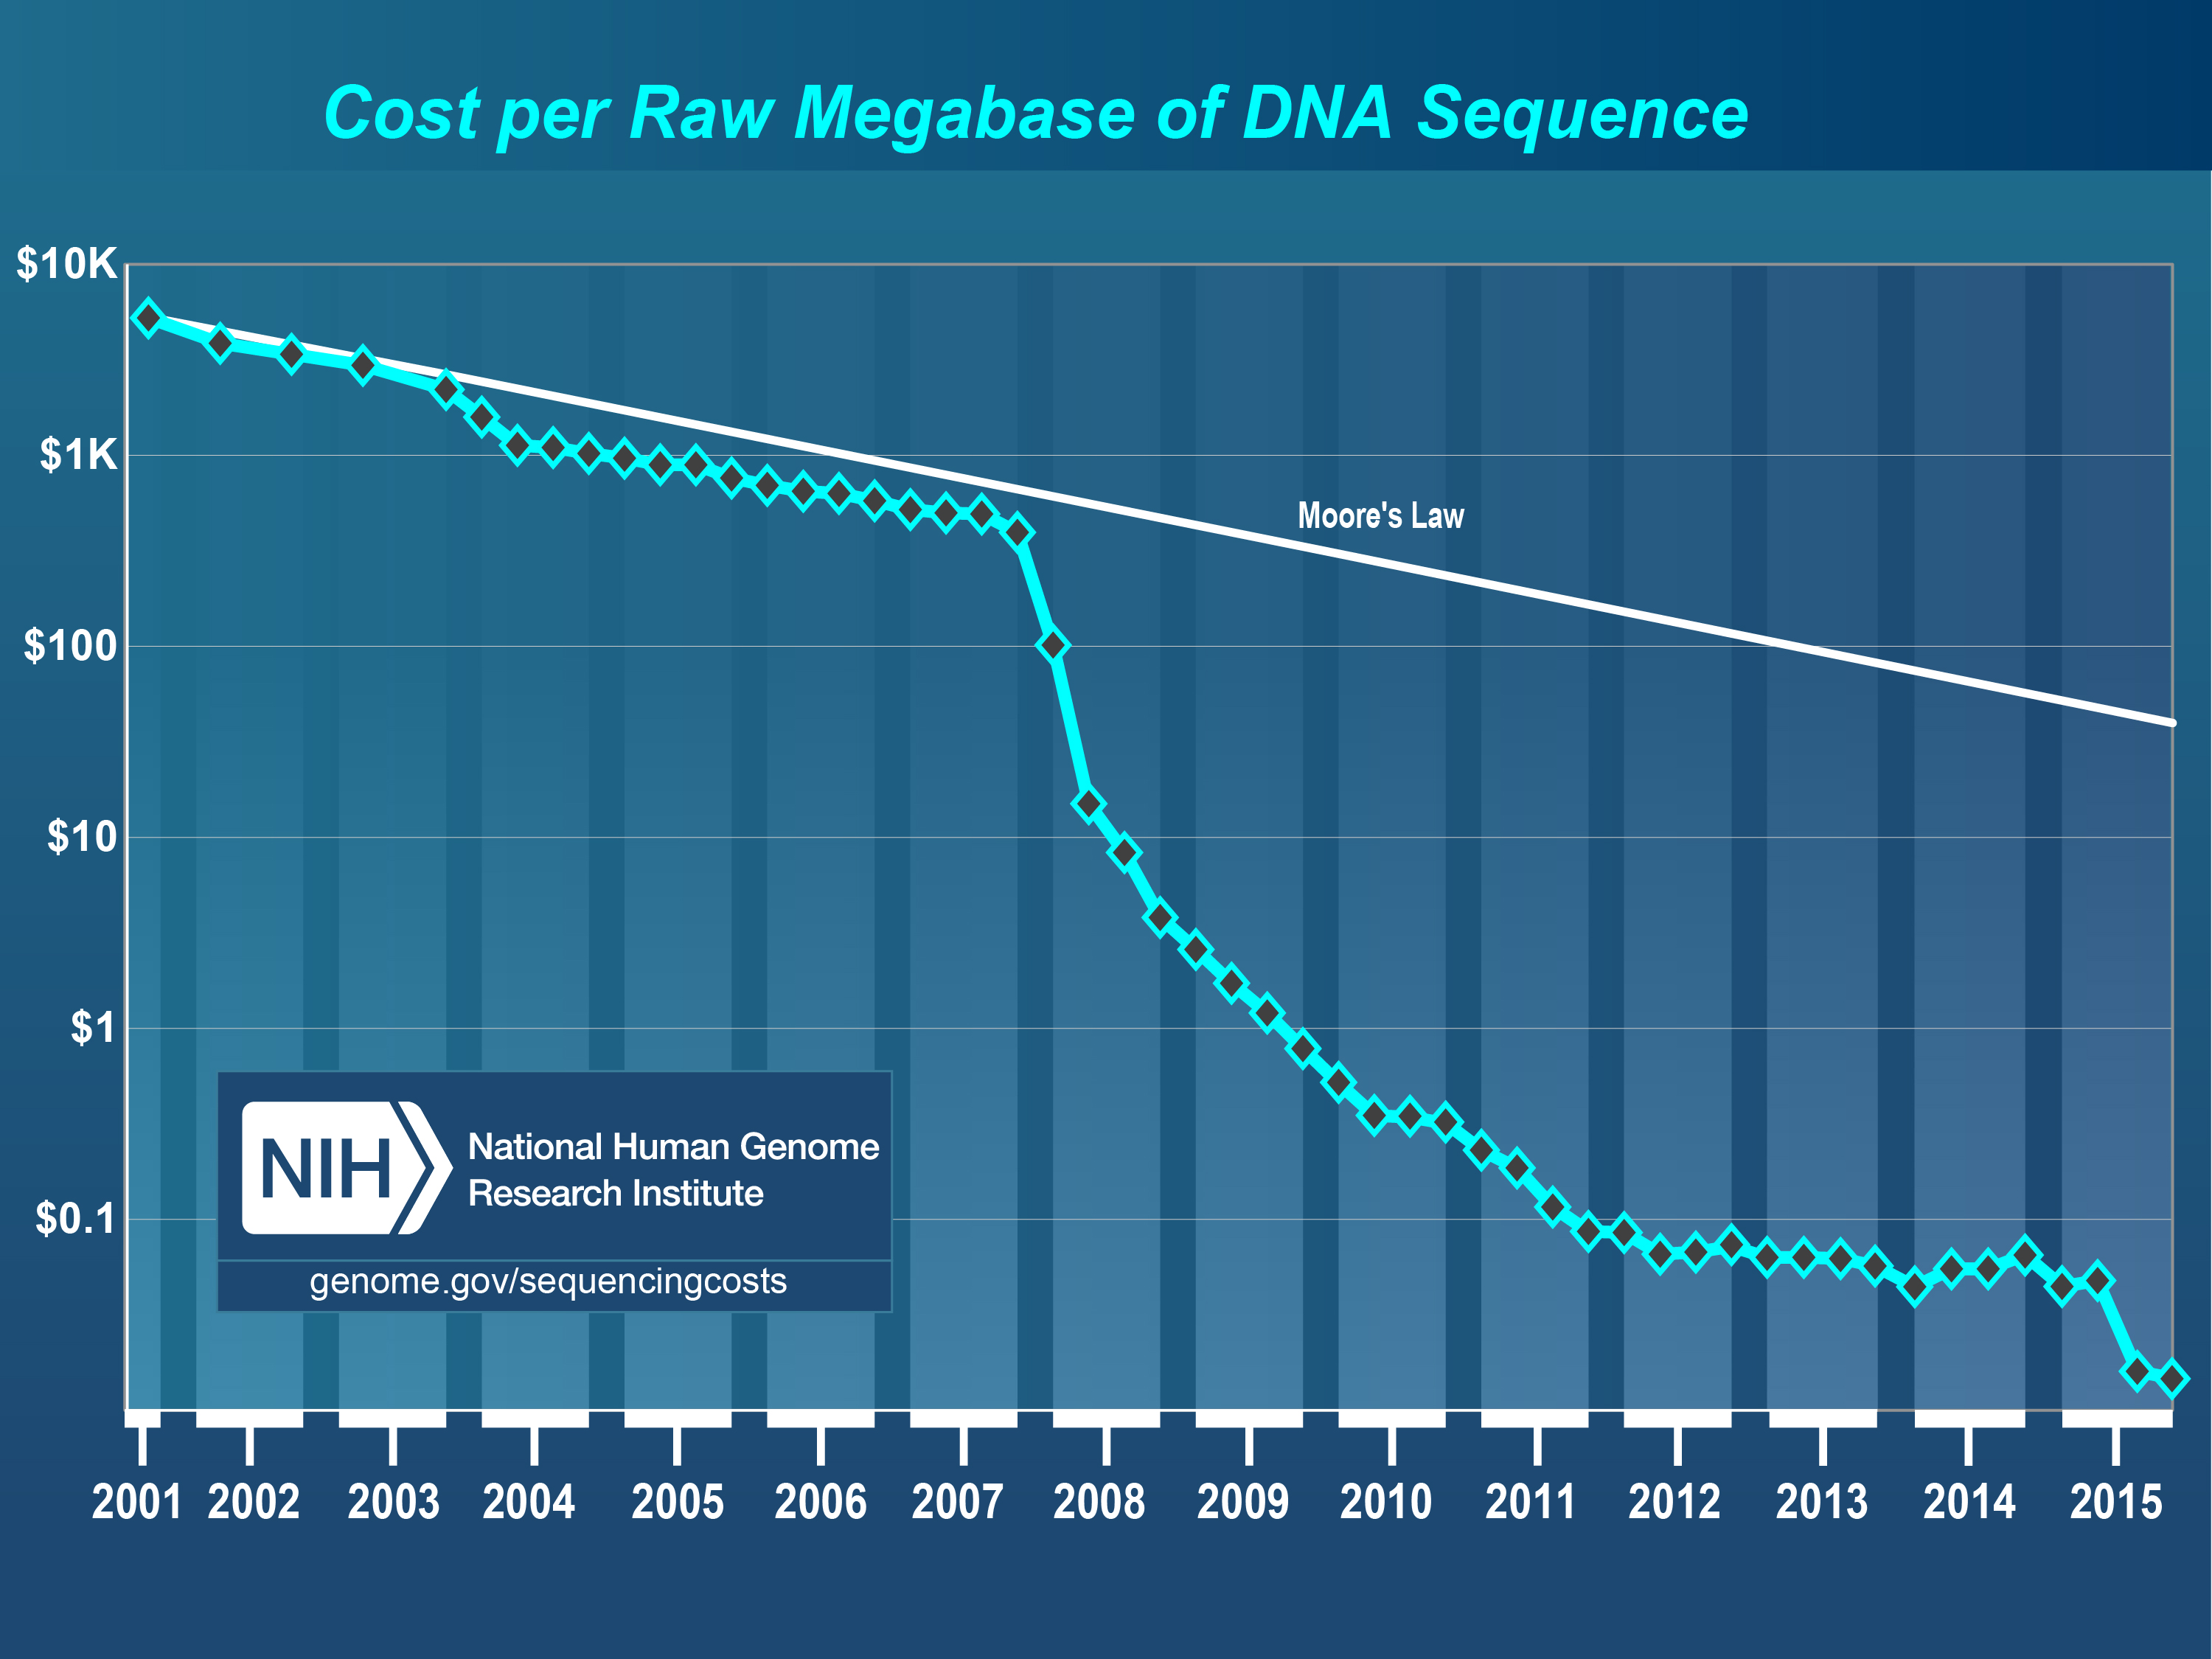
\includegraphics[scale=0.5]{costperMb2015_4.jpg}
\end{center}
\caption[Cost per raw megabase of DNA sequence from 2001 to 2015]{Cost per raw megabase of DNA sequence from 2001 to 2015. Straight line - Moore's Law, blue curve - cost in US dollars, Y-axis scale is logarithmic. Graph reproduced from \citep{wetterstrand2016}}
%Source:
\label{fig_dna_cost}
\end{figure}
Example of reference to a figure in the text (Fig.~\ref{fig_dna_cost}). Phasellus dolor neque, vehicula vestibulum semper at, facilisis eget libero. Mauris interdum magna molestie, auctor felis a, condimentum odio. Pellentesque habitant morbi tristique senectus et netus et malesuada fames ac turpis egestas. Suspendisse maximus lacinia dignissim. Maecenas pharetra accumsan metus, sagittis dictum purus sollicitudin eget. Curabitur ut porttitor arcu, ut porttitor ipsum. Vestibulum porttitor finibus sapien, ac pharetra odio bibendum nec. Nullam tincidunt dignissim risus imperdiet dictum.

Pellentesque habitant morbi tristique senectus et netus et malesuada fames ac turpis egestas. Suspendisse maximus lacinia dignissim. Maecenas pharetra accumsan metus, sagittis dictum purus sollicitudin eget. Curabitur ut porttitor arcu, ut porttitor ipsum. Vestibulum porttitor finibus sapien, ac pharetra odio bibendum nec. Nullam tincidunt dignissim risus imperdiet dictum.
\section{Example of a table}
Example of a table and here is the reference to Table \ref{table_genomes}. Tables in, my opinion, are the hardest thing to make.

\begin{table}
\begin{center}
\begin{tabular}{|l|c|c|c|}
\hline
{\sc Organism}  &  {\sc Accession no.}  & {\sc Genome size} (bp)  & {\sc No. CDS} \\
\hline
{\it Mesorhizobium loti}          & NC\_002678 & 7036071 & 6743 \\
\hline
{\it Sinorhizobium meliloti}      & NC\_003047 & 3654135 & 3359 \\
\hline
{\it Bradyrhizobium japonicum}    & NC\_004463 & 9105828 & 8317 \\
\hline
{\it Rhodopseudomonas palustris}  & NC\_005296 & 5459213 & 4813 \\
\hline
{\it Bartonella quintana}         & NC\_005955 & 1581384 & 1142 \\
\hline
{\it Bartonella henselae}         & NC\_005956 & 1931047 & 1488 \\
\hline
{\it Rickettsia typhi}            & NC\_006142 & 1111496 & 837 \\
\hline
{\it Beijerinckia indica}         & NC\_010581 & 4170153 & 3569 \\
\hline
\end{tabular}
\end{center}
\caption{Whole-genome sequences used in this study}
\label{table_genomes}
\end{table}

Fusce ultricies pulvinar diam sed ultrices. Sed orci justo, rutrum in dolor a, consequat dictum mi. Sed luctus congue ex nec dignissim. Phasellus volutpat urna vestibulum ipsum vestibulum, quis venenatis justo consectetur. Nullam hendrerit nisl in rutrum convallis. Sed sit amet malesuada nisi. Phasellus dolor neque, vehicula vestibulum semper at, facilisis eget libero. Mauris interdum magna molestie, auctor felis a, condimentum odio. Pellentesque habitant morbi tristique senectus et netus et malesuada fames ac turpis egestas. Suspendisse maximus lacinia dignissim. Maecenas pharetra accumsan metus, sagittis dictum purus sollicitudin eget. Curabitur ut porttitor arcu, ut porttitor ipsum. Vestibulum porttitor finibus sapien, ac pharetra odio bibendum nec. Nullam tincidunt dignissim risus imperdiet dictum.

Pellentesque habitant morbi tristique senectus et netus et malesuada fames ac turpis egestas. Suspendisse maximus lacinia dignissim. Maecenas pharetra accumsan metus, sagittis dictum purus sollicitudin eget. Curabitur ut porttitor arcu, ut porttitor ipsum. Vestibulum porttitor finibus sapien, ac pharetra odio bibendum nec. Nullam tincidunt dignissim risus imperdiet dictum.
\section{Chapter section}
Fusce ultricies pulvinar diam sed ultrices. Sed orci justo, rutrum in dolor a, consequat dictum mi. Sed luctus congue ex nec dignissim. Phasellus volutpat urna vestibulum ipsum vestibulum, quis venenatis justo consectetur. Nullam hendrerit nisl in rutrum convallis. Sed sit amet malesuada nisi. Phasellus dolor neque, vehicula vestibulum semper at, facilisis eget libero. Mauris interdum magna molestie, auctor felis a, condimentum odio. Pellentesque habitant morbi tristique senectus et netus et malesuada fames ac turpis egestas. Suspendisse maximus lacinia dignissim. Maecenas pharetra accumsan metus, sagittis dictum purus sollicitudin eget. Curabitur ut porttitor arcu, ut porttitor ipsum. Vestibulum porttitor finibus sapien, ac pharetra odio bibendum nec. Nullam tincidunt dignissim risus imperdiet dictum.

Pellentesque habitant morbi tristique senectus et netus et malesuada fames ac turpis egestas. Suspendisse maximus lacinia dignissim. Maecenas pharetra accumsan metus, sagittis dictum purus sollicitudin eget. Curabitur ut porttitor arcu, ut porttitor ipsum. Vestibulum porttitor finibus sapien, ac pharetra odio bibendum nec. Nullam tincidunt dignissim risus imperdiet dictum.


% Bibliography
\begingroup
\setlength\bibitemsep{10pt}
\linespread{1}\selectfont
\cleardoublepage
\phantomsection
\addcontentsline{toc}{part}{REFERENCES}
\printbibliography[title=REFERENCES]
\endgroup



% Appendices
\appendix

%%%%%%%%%% DON'T DELETE THIS, REVERTS NUMBERING BACK %%%%%%%%%%%%%
\makeatletter
\renewcommand{\@makechapterhead}[1]{\vspace *{-10\p@ }{\parindent \z@ 
\raggedright \normalfont \ifnum \c@secnumdepth >\m@ne \Huge \bfseries 
\@chapapp \space \thechapter \vskip 10\p@ \fi #1\par \nobreak \vskip 30\p@ }}
\makeatother
%%%%%%%%%% DON'T DELETE THIS, REVERTS NUMBERING BACK %%%%%%%%%%%%%

\chapter{Reciprocal Lattice and Brillouin Zone}\label{chap:BZ}
Reciprocal lattice vectors of a lattice are defined to be the wavevectors  $\va{G}$ that satisfy 
\begin{equation} \label{eq:GdotR}
    \exp(i \va{G} \vdot \va{R} ) = 1
\end{equation}
for any lattice translation vector $\va{R}$ given by
\begin{equation}
    \va{R} = n_1 \va{a}_1 + n_2 \va{a}_2 +n_3 \va{a}_3
\end{equation}
Here $n_1, n_2, n_3$ are arbitrary integers and $\va{a}_1, \va{a}_2, \va{a}_3$ are the primitive lattice vectors of the direct (real) lattice. Similarly, the reciprocal lattice vector can be resolved into its components 
\begin{equation}
    \va{G} = h \va{b}_1 + k \va{b}_2 + l \va{b}_3
\end{equation}
where $h, k, l$ are also  arbitrary integers and $\va{b}_1, \va{b}_2, \va{b}_3$ are the primitive lattice vectors of the reciprocal lattice. The integers $h, k, l$ constitute the so called Miller indices $(hkl)$. Satisfying \eqref{eq:GdotR} means that 
\begin{equation*}
    \va{a}_i \vdot \va{b}_j = 2 \pi \delta_{ij}
\end{equation*}
It can be shown that the reciprocal vectors $b_j$ can be constructed entirely in terms of real vectors $a_i$
\begin{align}
    \va{b}_1 &= 2 \pi \frac{\va{a}_2 \crossproduct \va{a}_3}{V} \\
    \va{b}_2 &= 2 \pi \frac{\va{a}_3 \crossproduct \va{a}_1}{V} \\
    \va{b}_3 &= 2 \pi \frac{\va{a}_1 \crossproduct \va{a}_2}{V} 
\end{align}
where $V = \va{a}_1 \vdot (\va{a}_2 \crossproduct \va{a}_3)$ is the volume of the unit cell. Reciprocal lattice and real lattice have important relationship. It can be shown that the reciprocal lattice vector defined by the Miller indices $(hkl)$ are perpendicular to the direct (real) lattice plane whose intercepts are the reciprocals of Miller indices $(hkl)$. 

The Brillouin Zone (BZ) is defined to be the primitive unit cell of the reciprocal lattice. The first BZ is the Wigner-Seitz cell around the wavevector $\va{k}=0$, the origin of the reciprocal space, which is defined to be the region of reciprocal space closer to $\va{k}=0$ than to any other reciprocal lattice vector. Similarly, all wavevectors that are second closest to $\va{k}=0$, constitute the second BZ, and so forth. The Wigner-Seitz cell contains only one reciprocal lattice point in it. This means that first BZ is constructed as the smallest volume entirely closed by a set of planes that are the perpendicular bisectors of the origin to each reciprocal lattice vectors. The volume of the first BZ is  related to the volume of the primitive unit cell of the real lattice
\begin{equation}
    \Omega = \frac{(2\pi)^3}{V}
\end{equation}

Brillouin zone plays a vital role in calculation of periodic systems. Owing to the periodic nature of the reciprocal lattice, any wavevectors $\va{k}$ outside the first BZ can be folded back into the first BZ by a reciprocal lattice vector $\va{G}$. In addition, any wavevectors that are shifted by a reciprocal lattice vector are all equivalent. Hence, any physical properties that have periodicity of the crystal system can be represented entirely inside the first Brillouin zone. 



















\newpage
\vspace*{-0.3in}
\begin{figure}[hb!]
\begin{center}
\makebox[\textwidth][c]{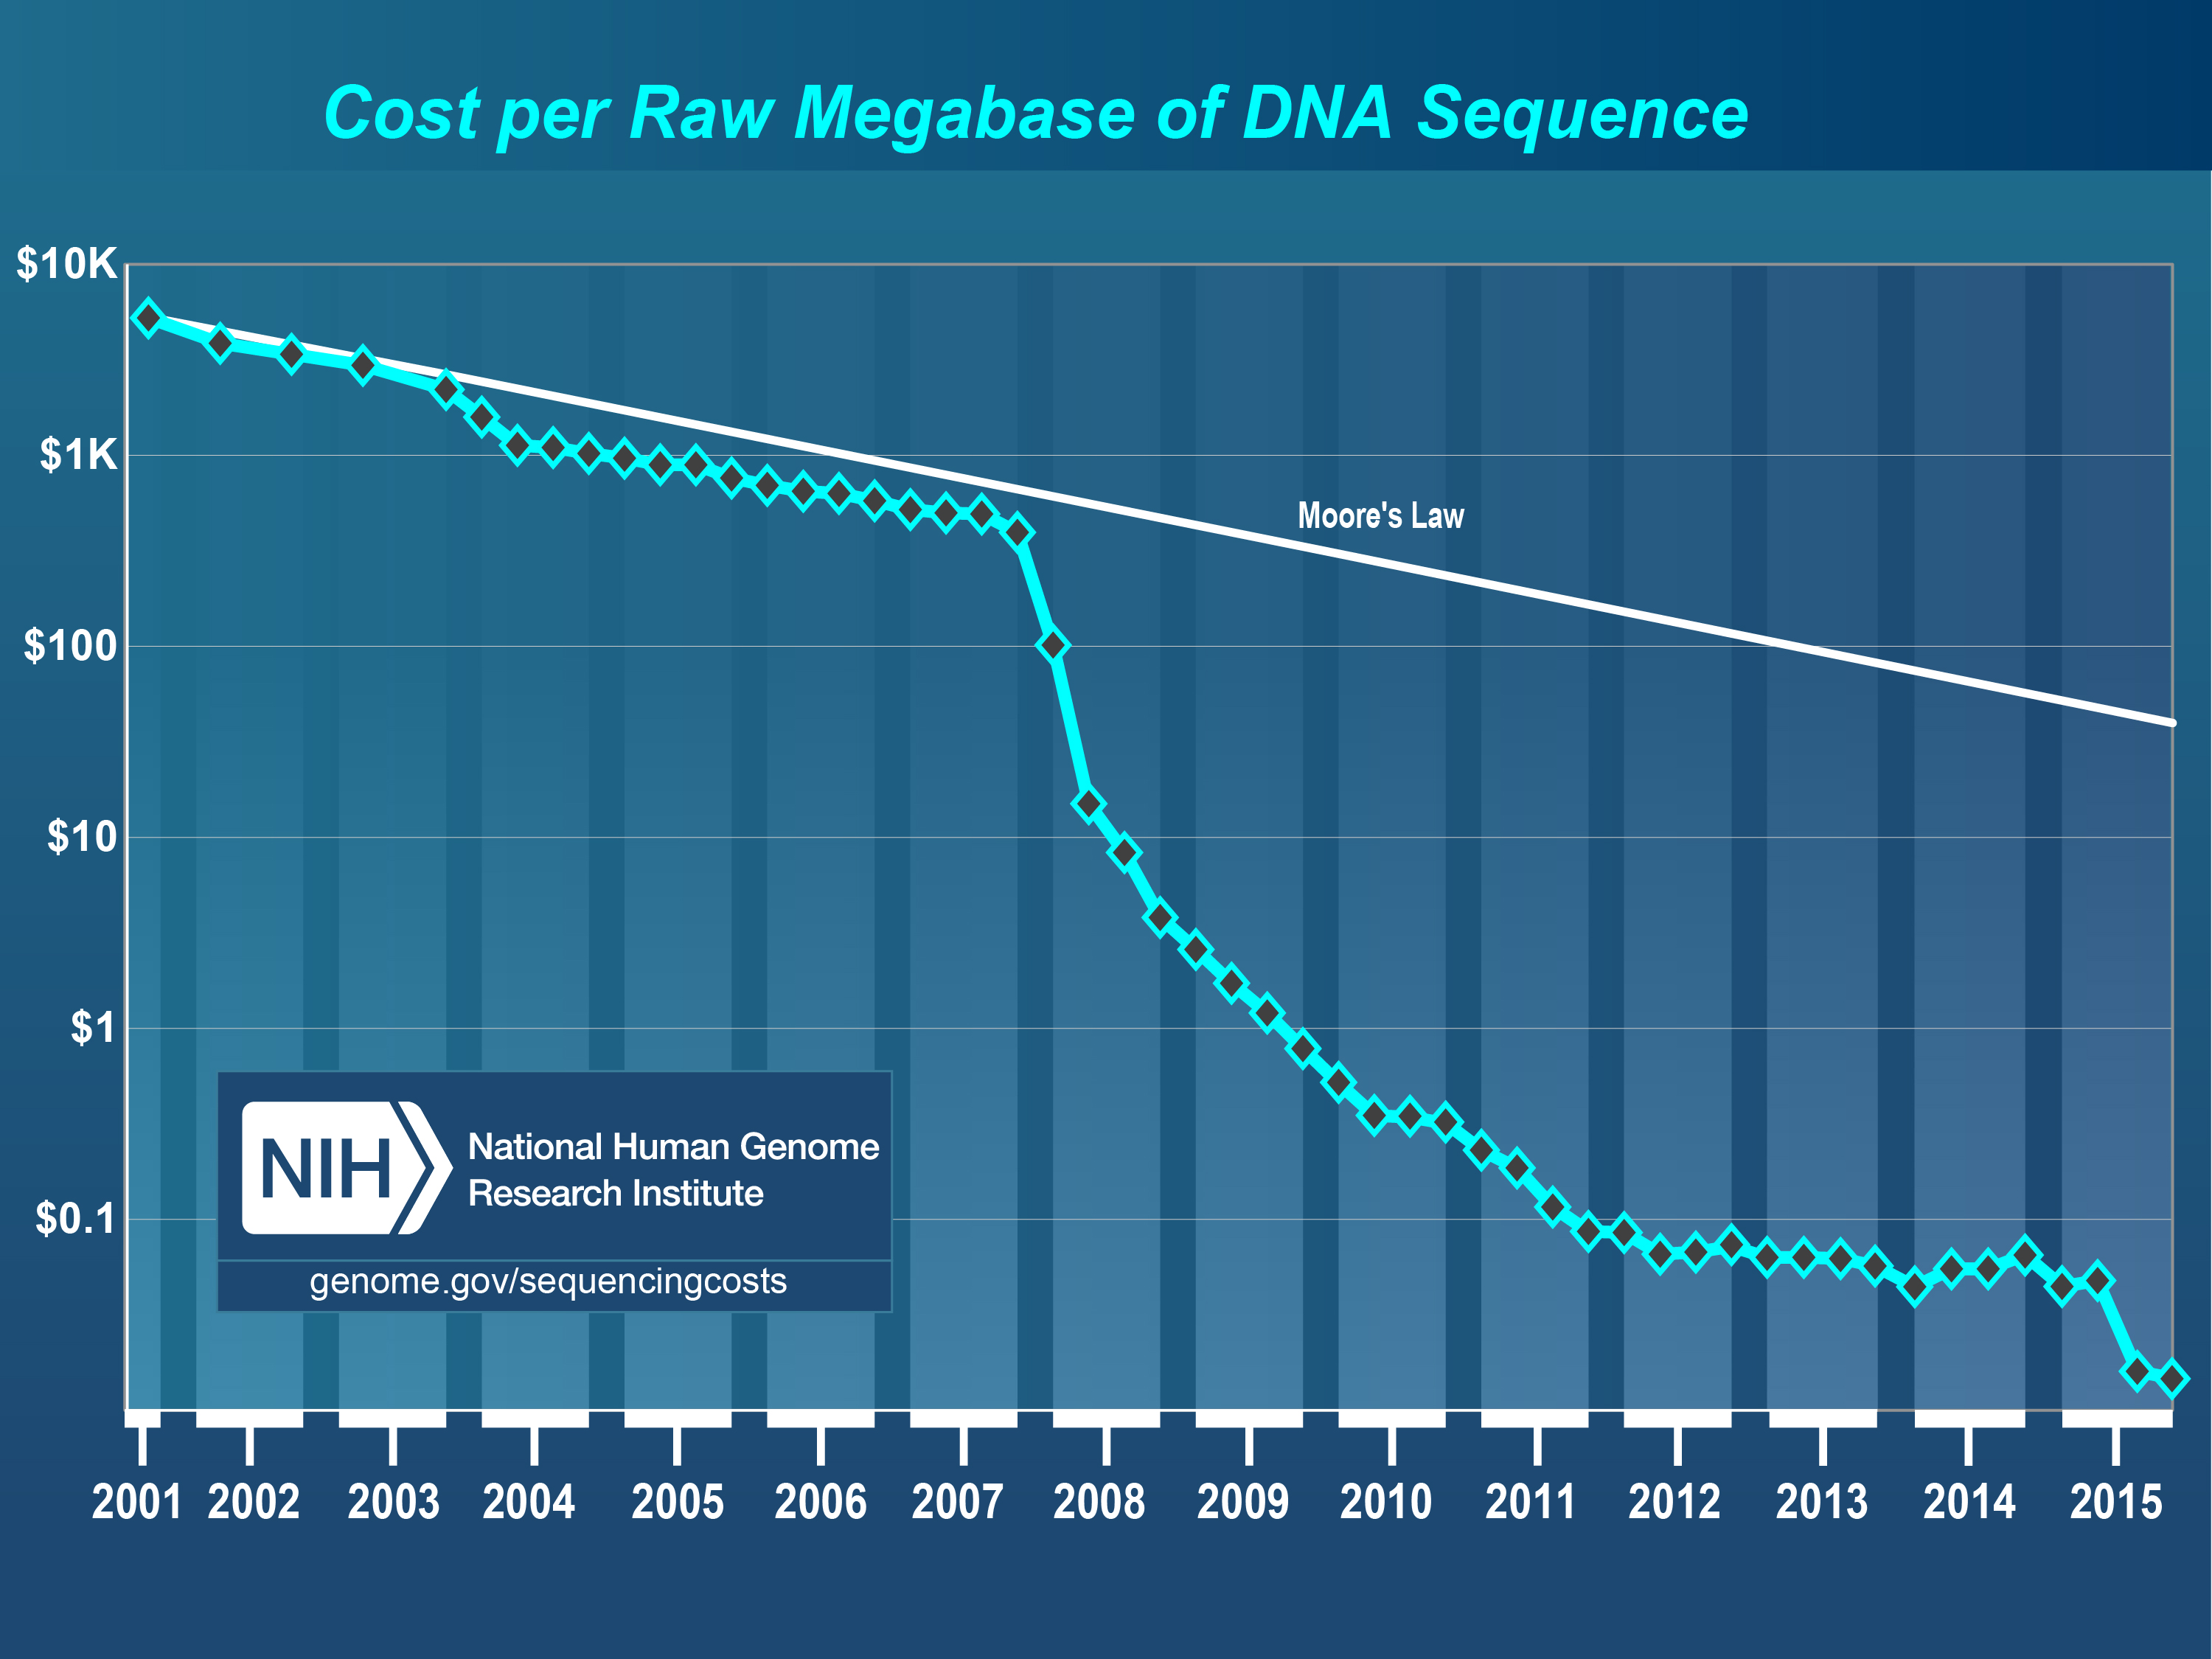
\includegraphics[width=1.0\textwidth]{costperMb2015_4.jpg}}
\end{center}
\caption[Cost per raw megabase of DNA sequence from 2001 to 2015]{Cost per raw megabase of DNA sequence from 2001 to 2015. Straight line - Moore's Law, blue curve - cost in US dollars, Y-axis scale is logarithmic. Graph reproduced from \citep{wetterstrand2016}}
\end{figure}
\begin{figure}[hb!]
\begin{center}
\makebox[\textwidth][c]{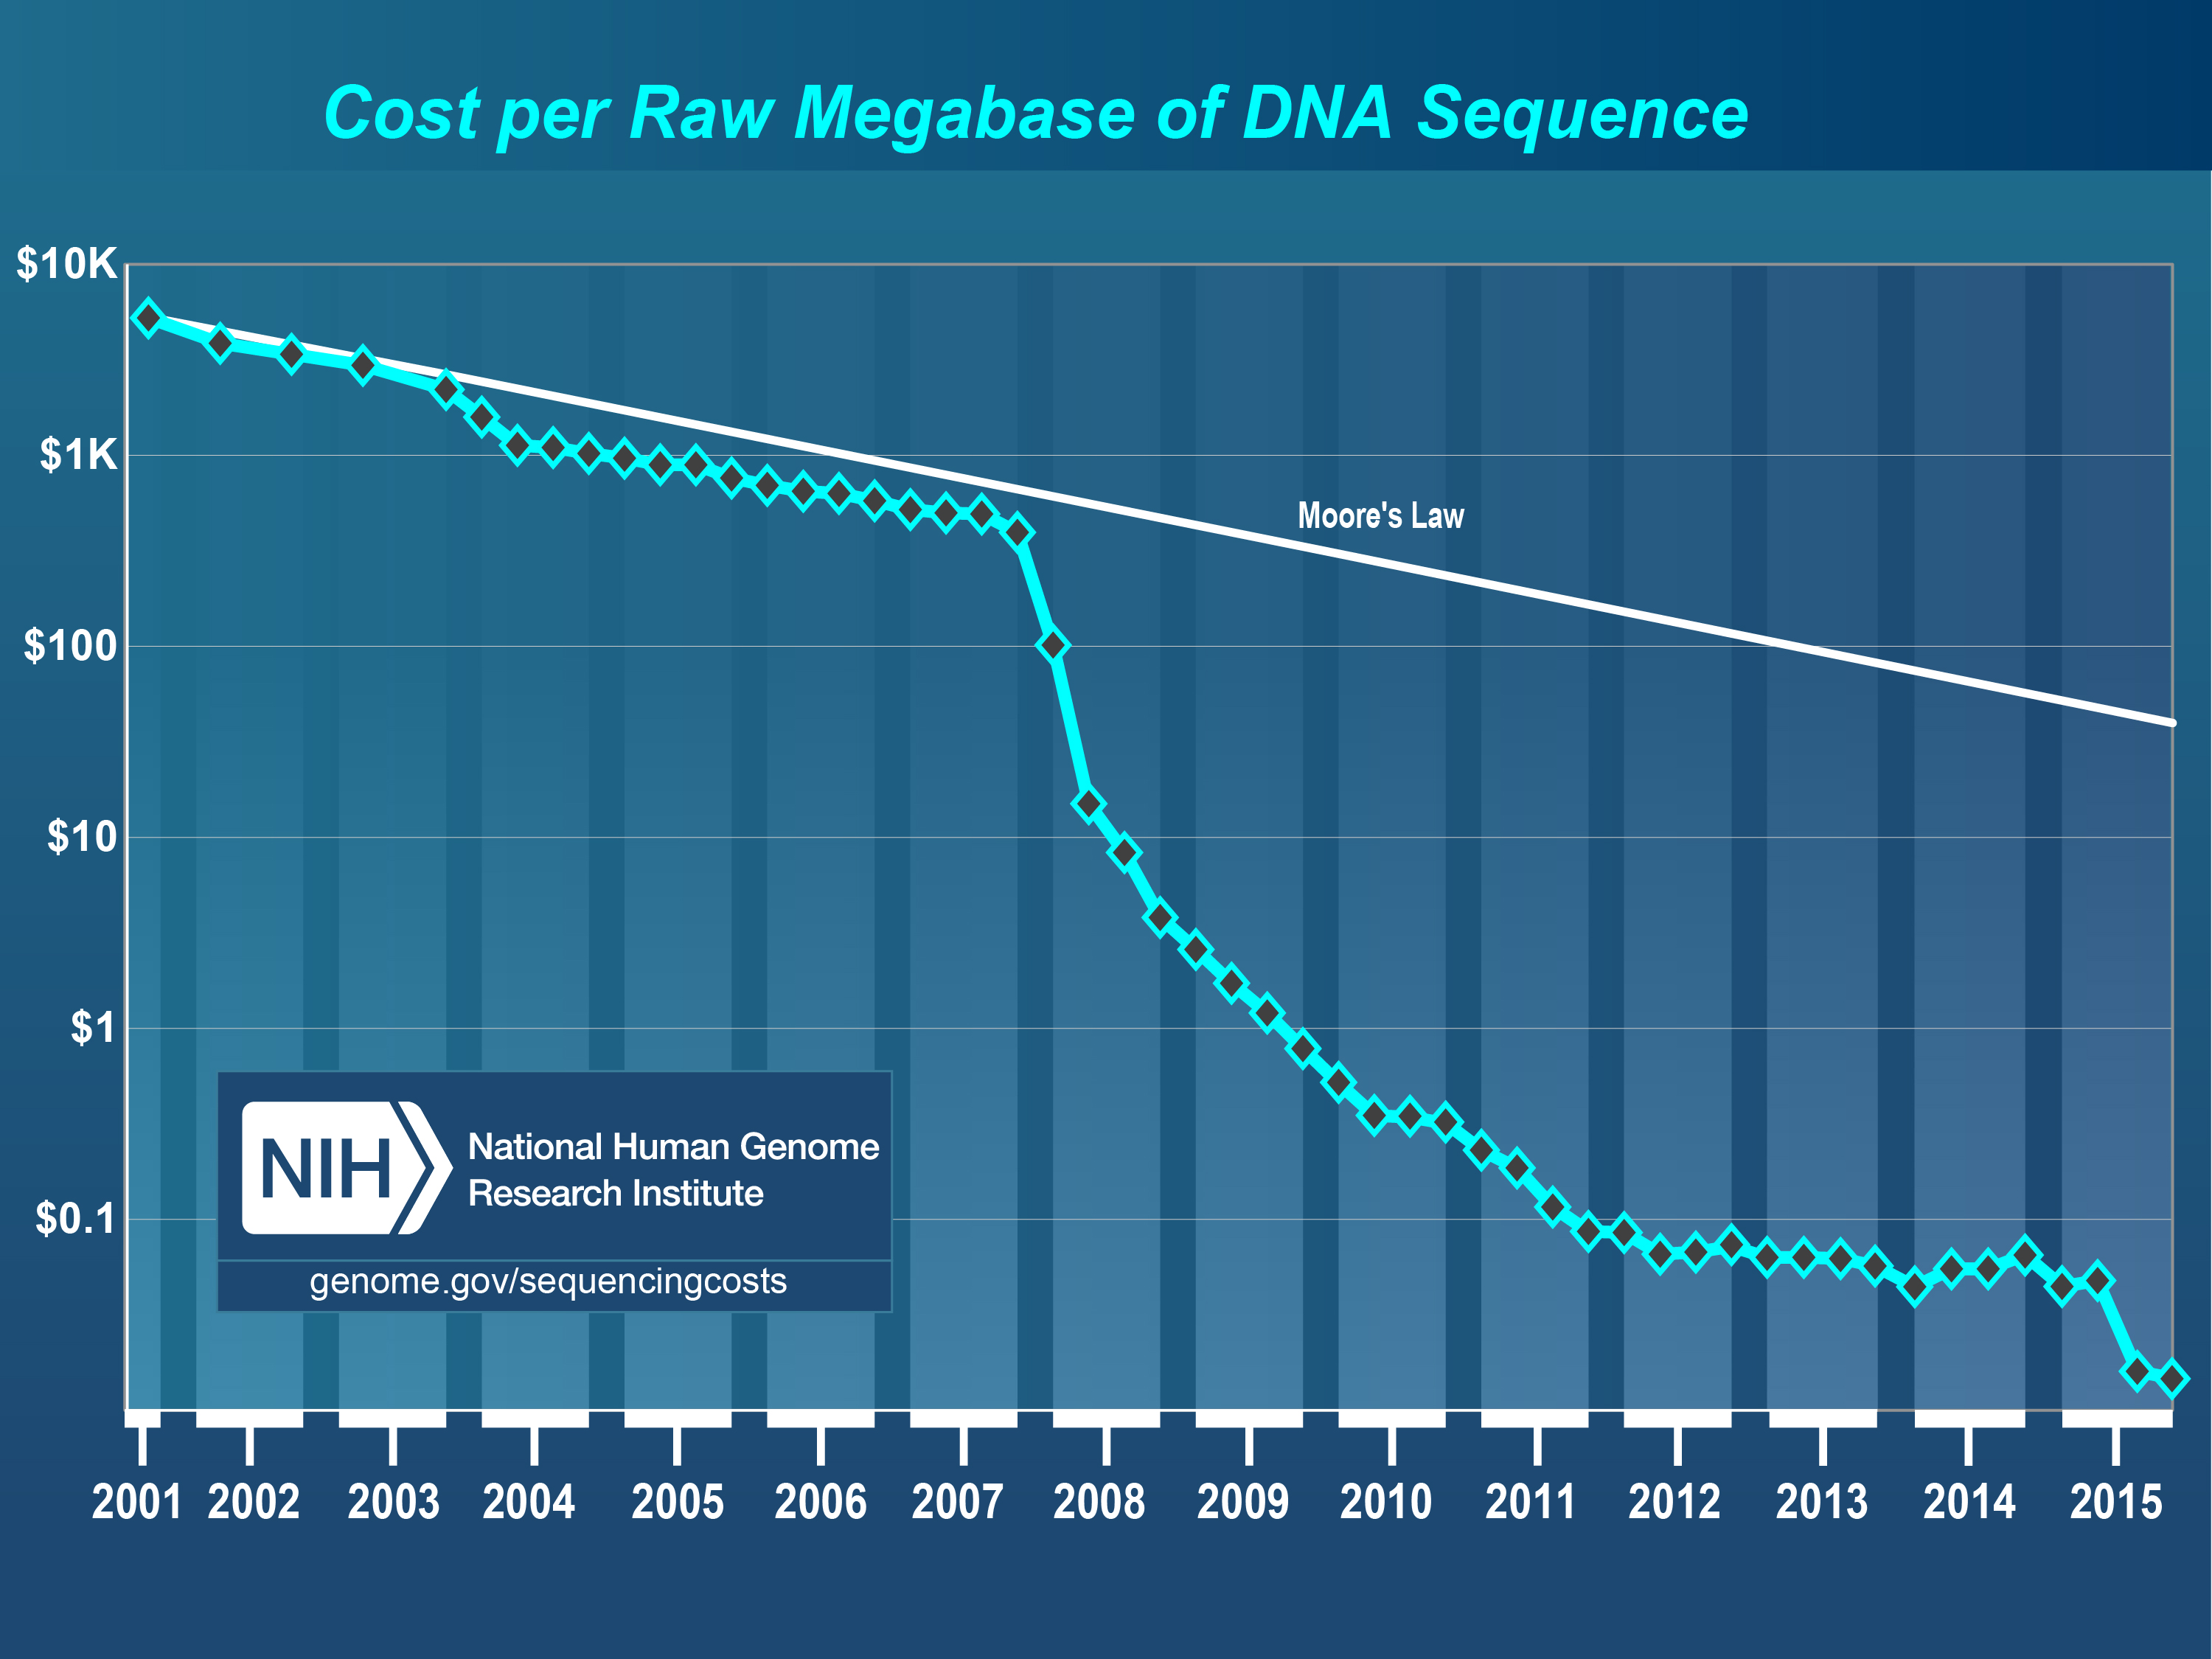
\includegraphics[width=1.0\textwidth]{costperMb2015_4.jpg}}
\end{center}
\caption[Cost per raw megabase of DNA sequence from 2001 to 2015]{Cost per raw megabase of DNA sequence from 2001 to 2015. Straight line - Moore's Law, blue curve - cost in US dollars, Y-axis scale is logarithmic. Graph reproduced from \citep{wetterstrand2016}}
\end{figure}

\chapter{}
\vspace*{-0.3in}
\begin{figure}[hb!]
\begin{center}
\makebox[\textwidth][c]{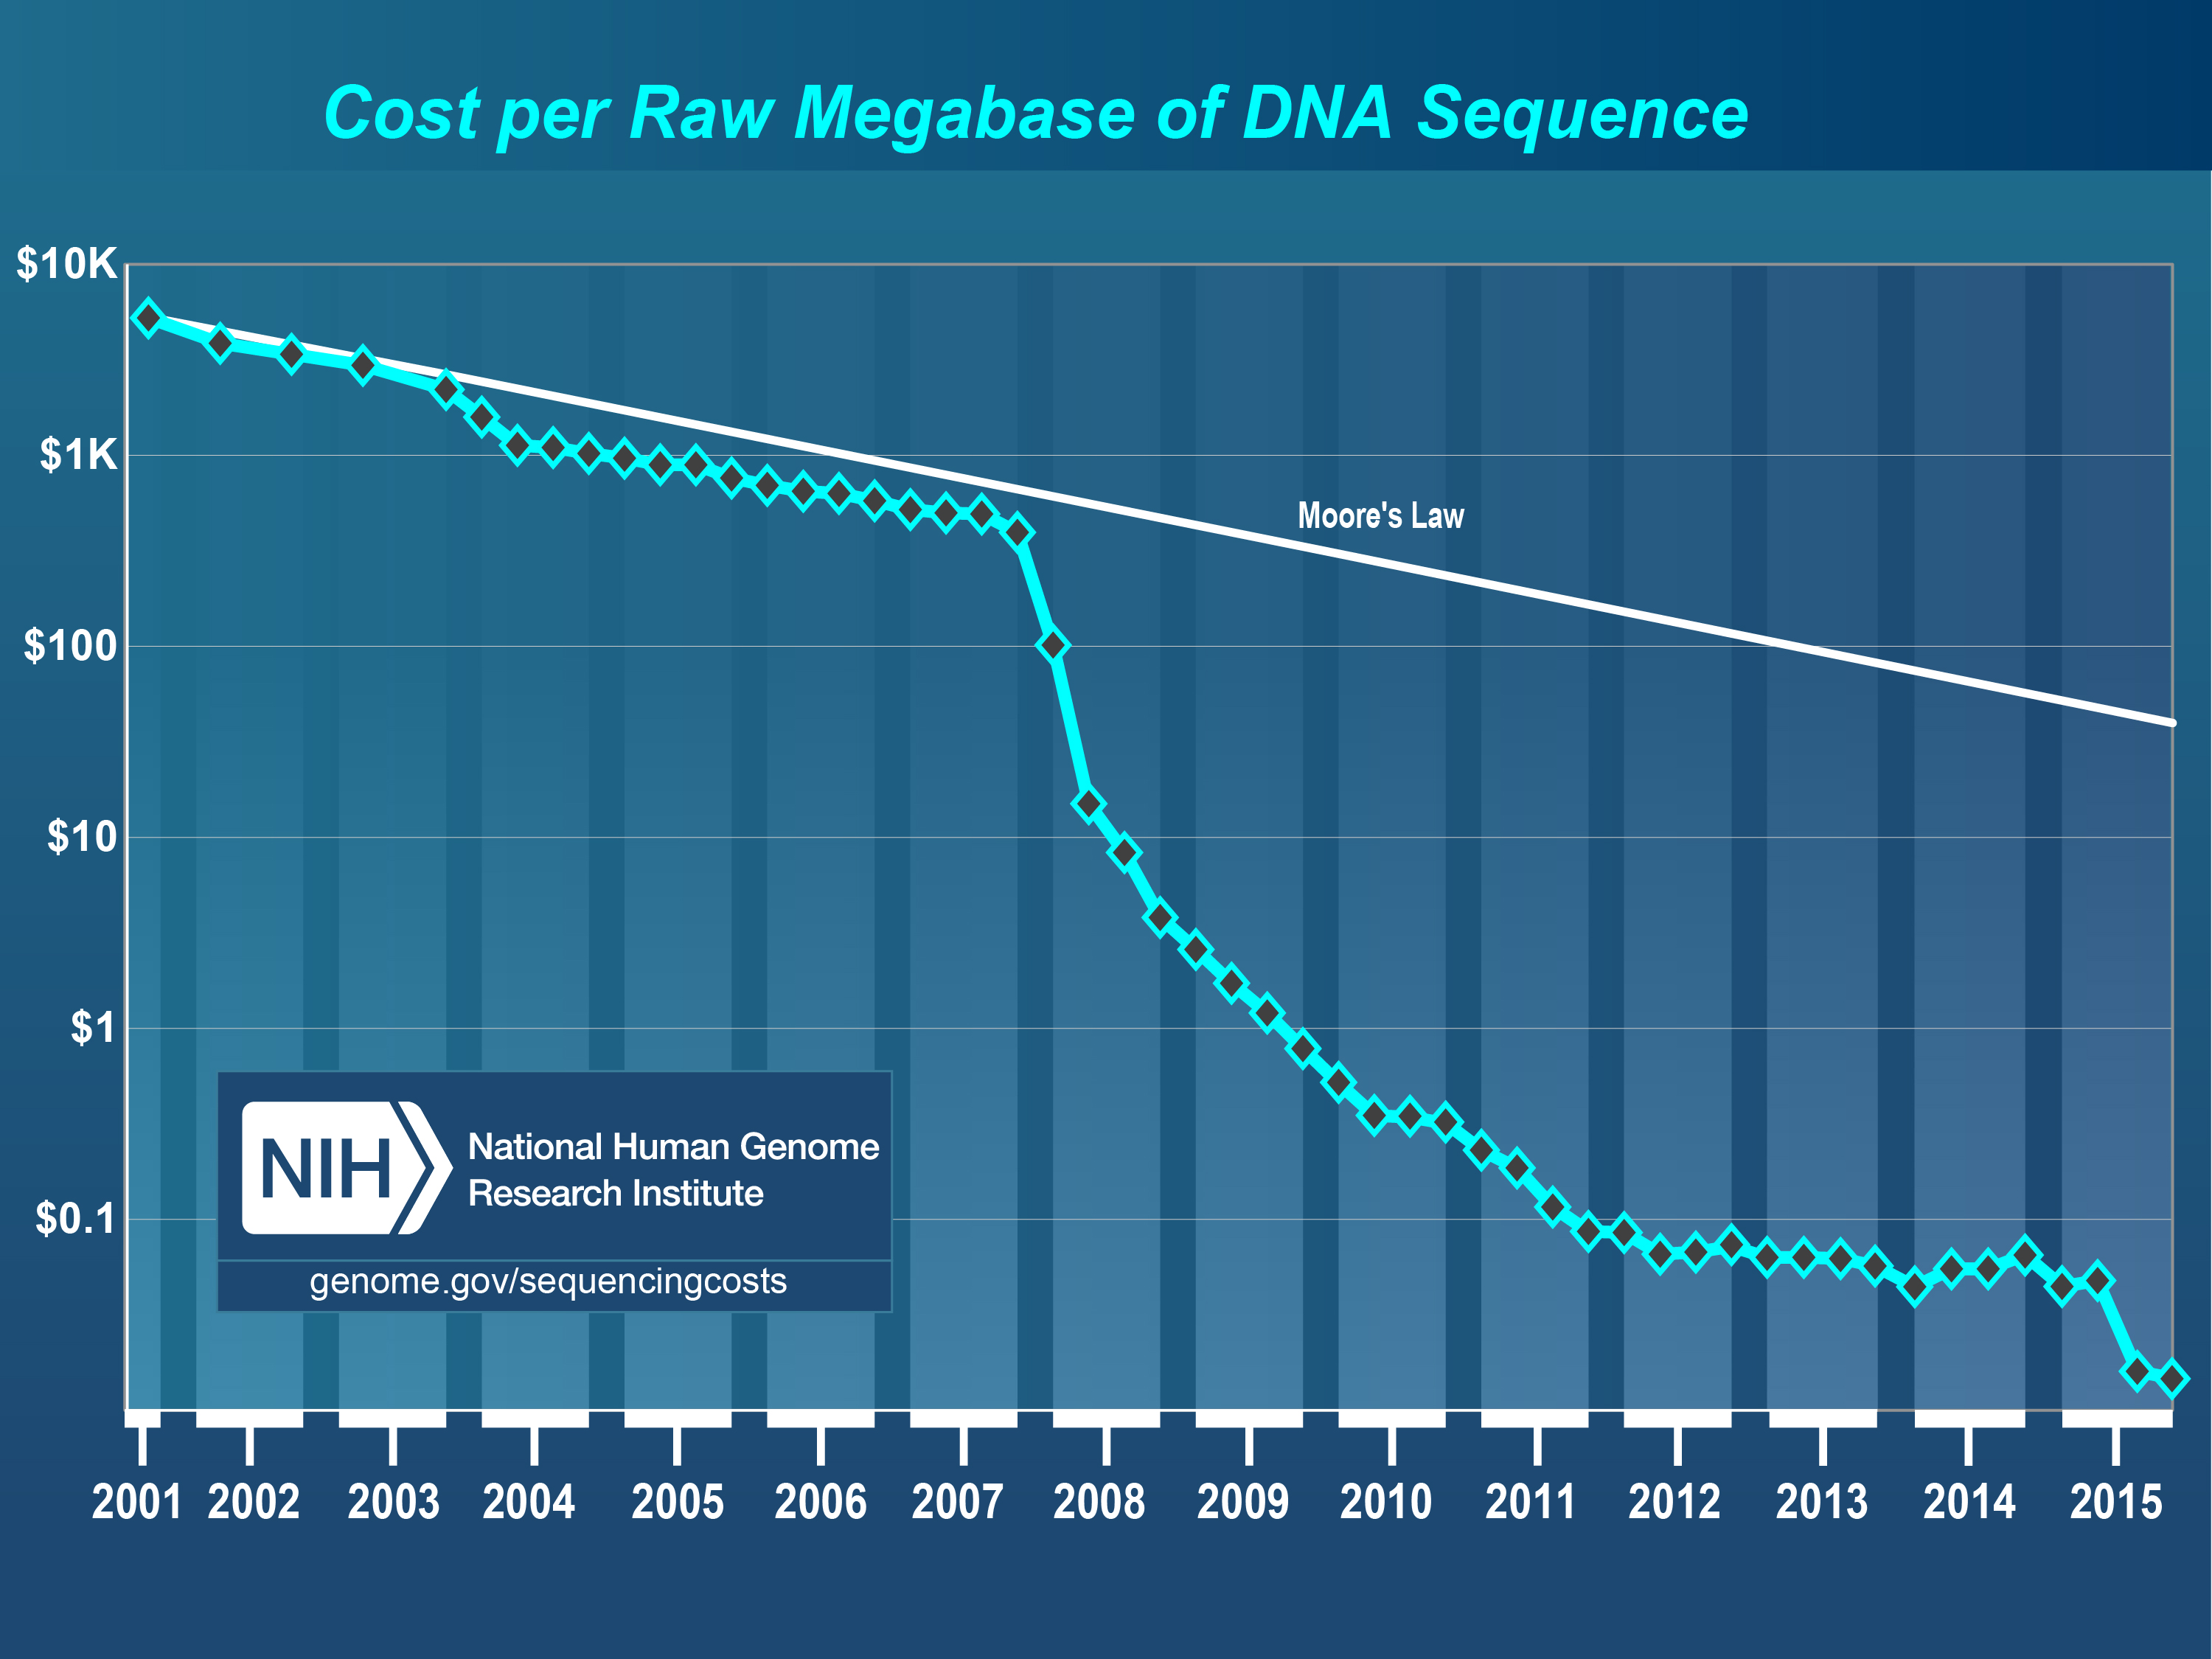
\includegraphics[width=1.0\textwidth]{costperMb2015_4.jpg}}
\end{center}
\caption[Cost per raw megabase of DNA sequence from 2001 to 2015]{Cost per raw megabase of DNA sequence from 2001 to 2015. Straight line - Moore's Law, blue curve - cost in US dollars, Y-axis scale is logarithmic. Graph reproduced from \citep{wetterstrand2016}}
\end{figure}

\chapter{}
\begin{figure}[hb!]
\begin{center}
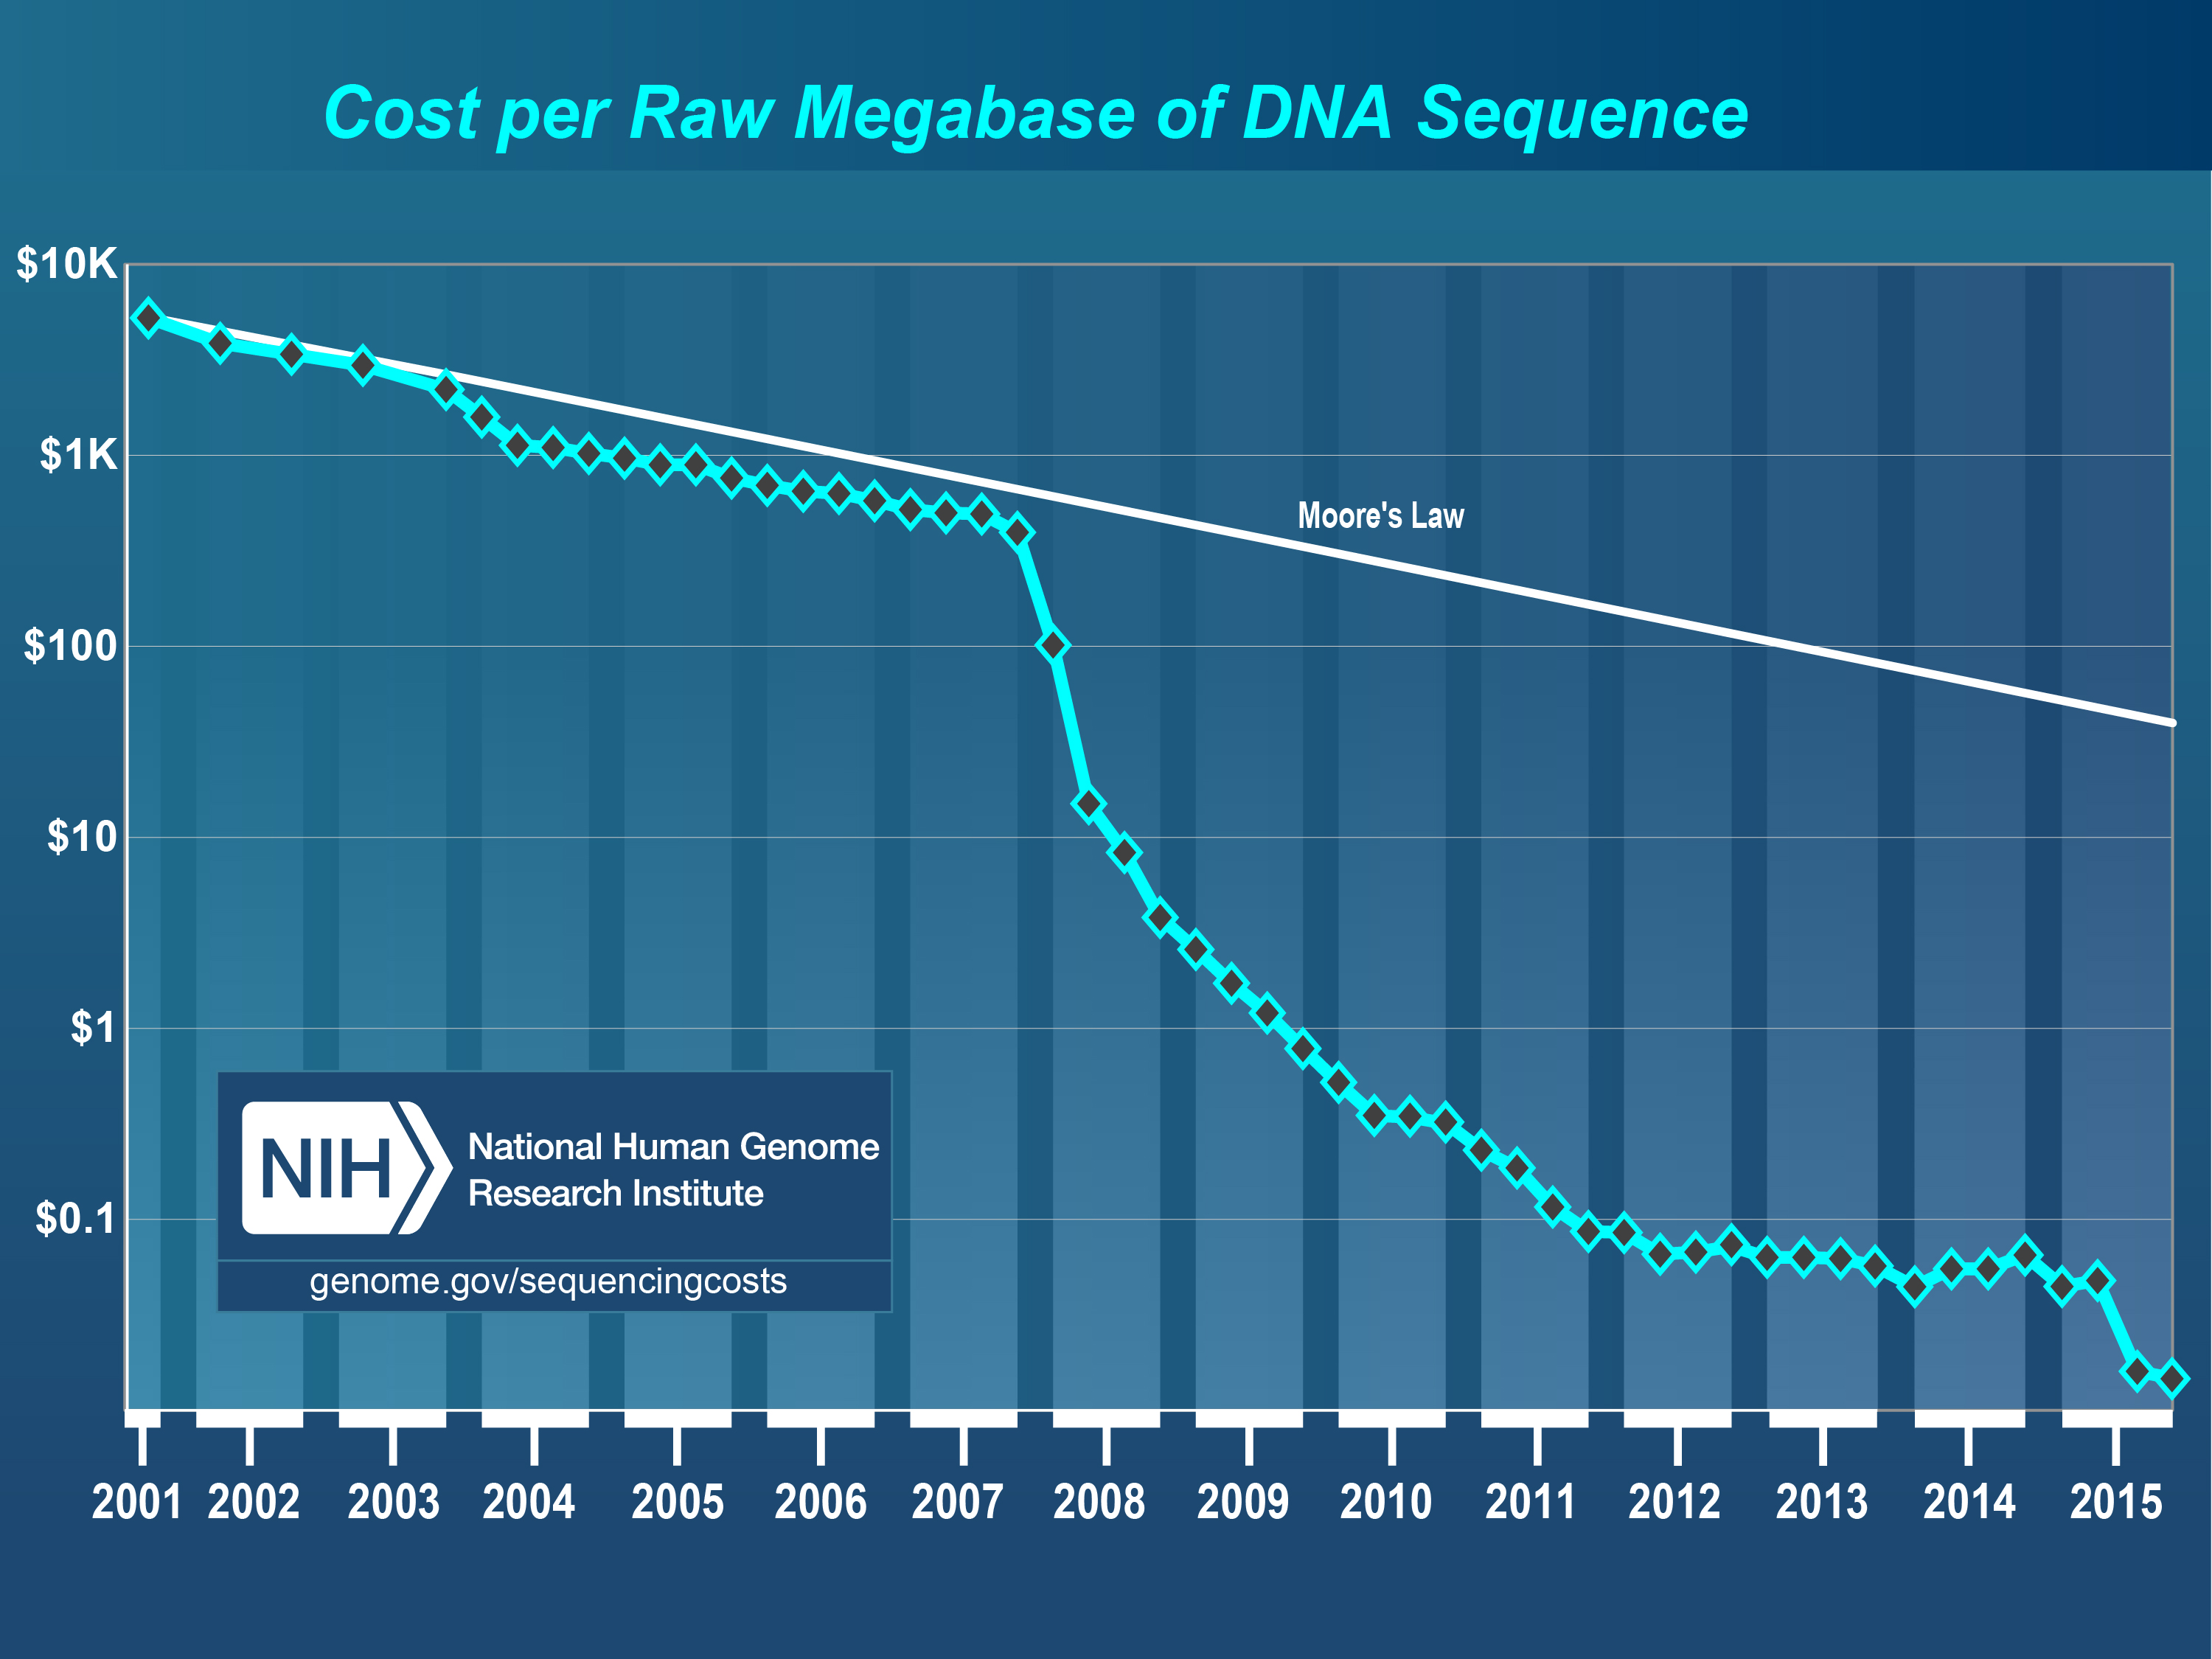
\includegraphics[scale=0.5]{costperMb2015_4.jpg}
\end{center}
\caption[Cost per raw megabase of DNA sequence from 2001 to 2015]{Cost per raw megabase of DNA sequence from 2001 to 2015. Straight line - Moore's Law, blue curve - cost in US dollars, Y-axis scale is logarithmic. Graph reproduced from \citep{wetterstrand2016}}
\end{figure}

\chapter{}
\begin{figure}[hb!]
\begin{center}
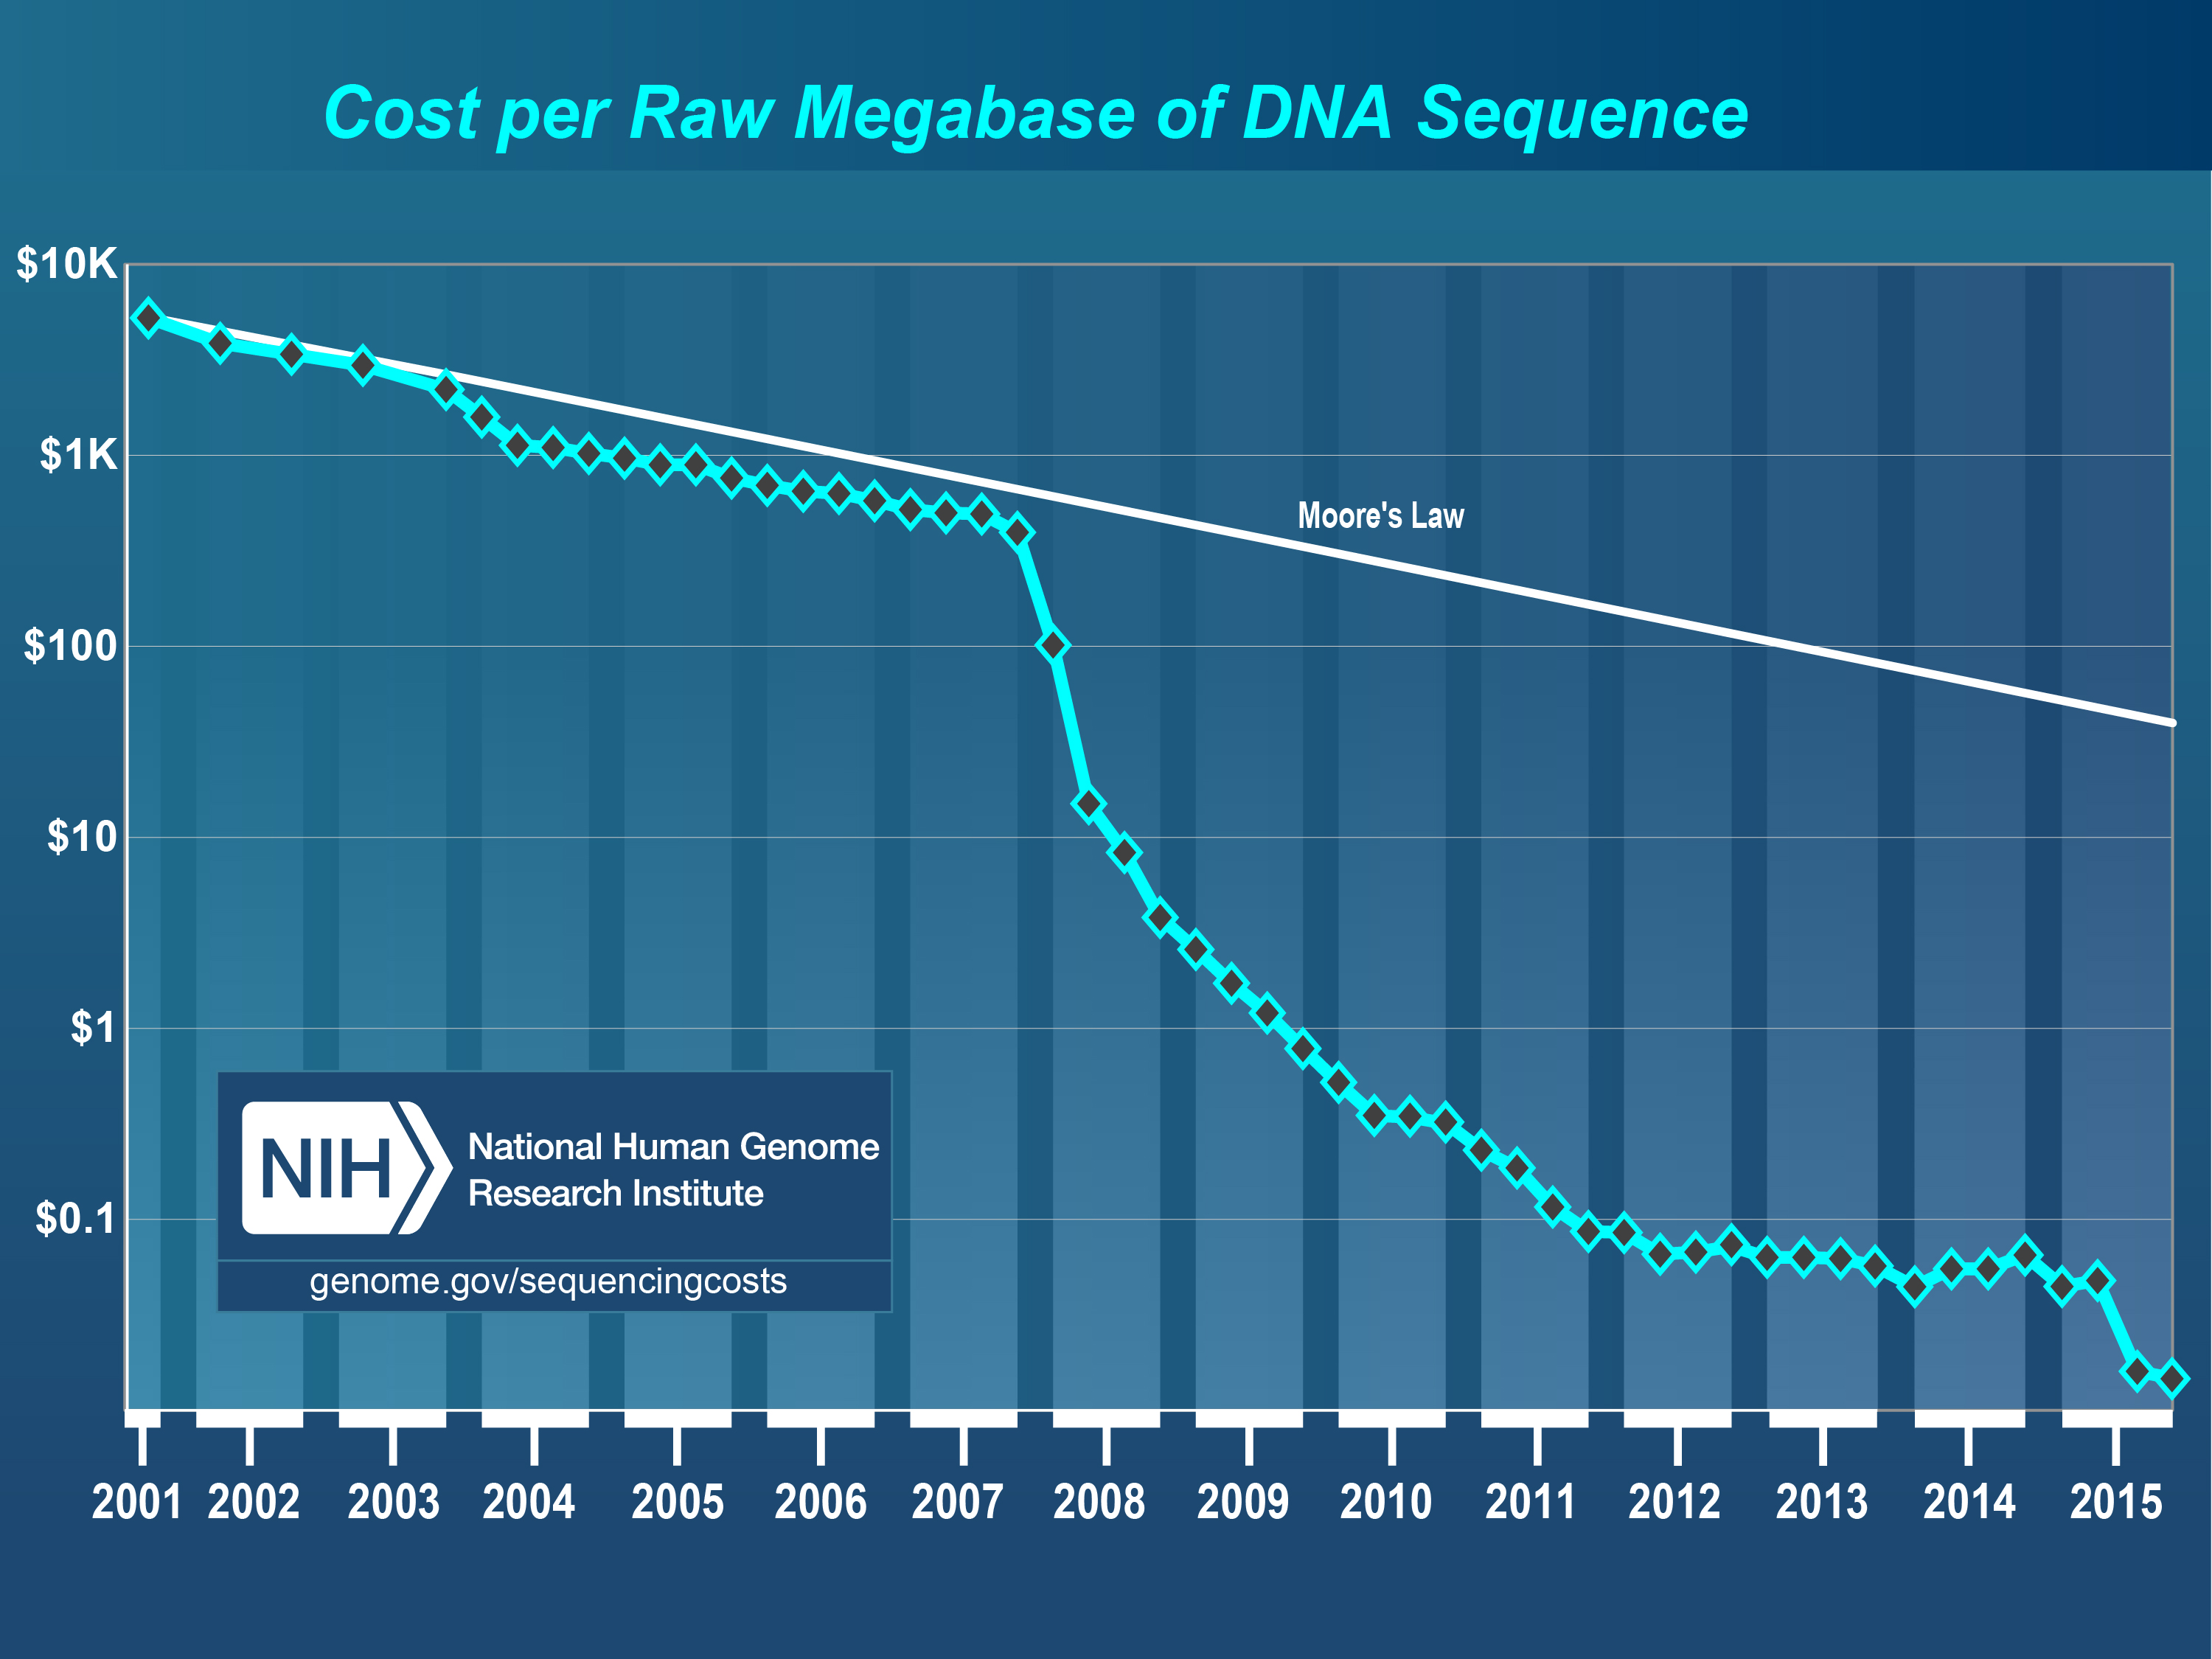
\includegraphics[scale=0.5]{costperMb2015_4.jpg}
\end{center}
\caption[Cost per raw megabase of DNA sequence from 2001 to 2015]{Cost per raw megabase of DNA sequence from 2001 to 2015. Straight line - Moore's Law, blue curve - cost in US dollars, Y-axis scale is logarithmic. Graph reproduced from \citep{wetterstrand2016}}
\end{figure}

\chapter{}
\begin{figure}[hb!]
\begin{center}
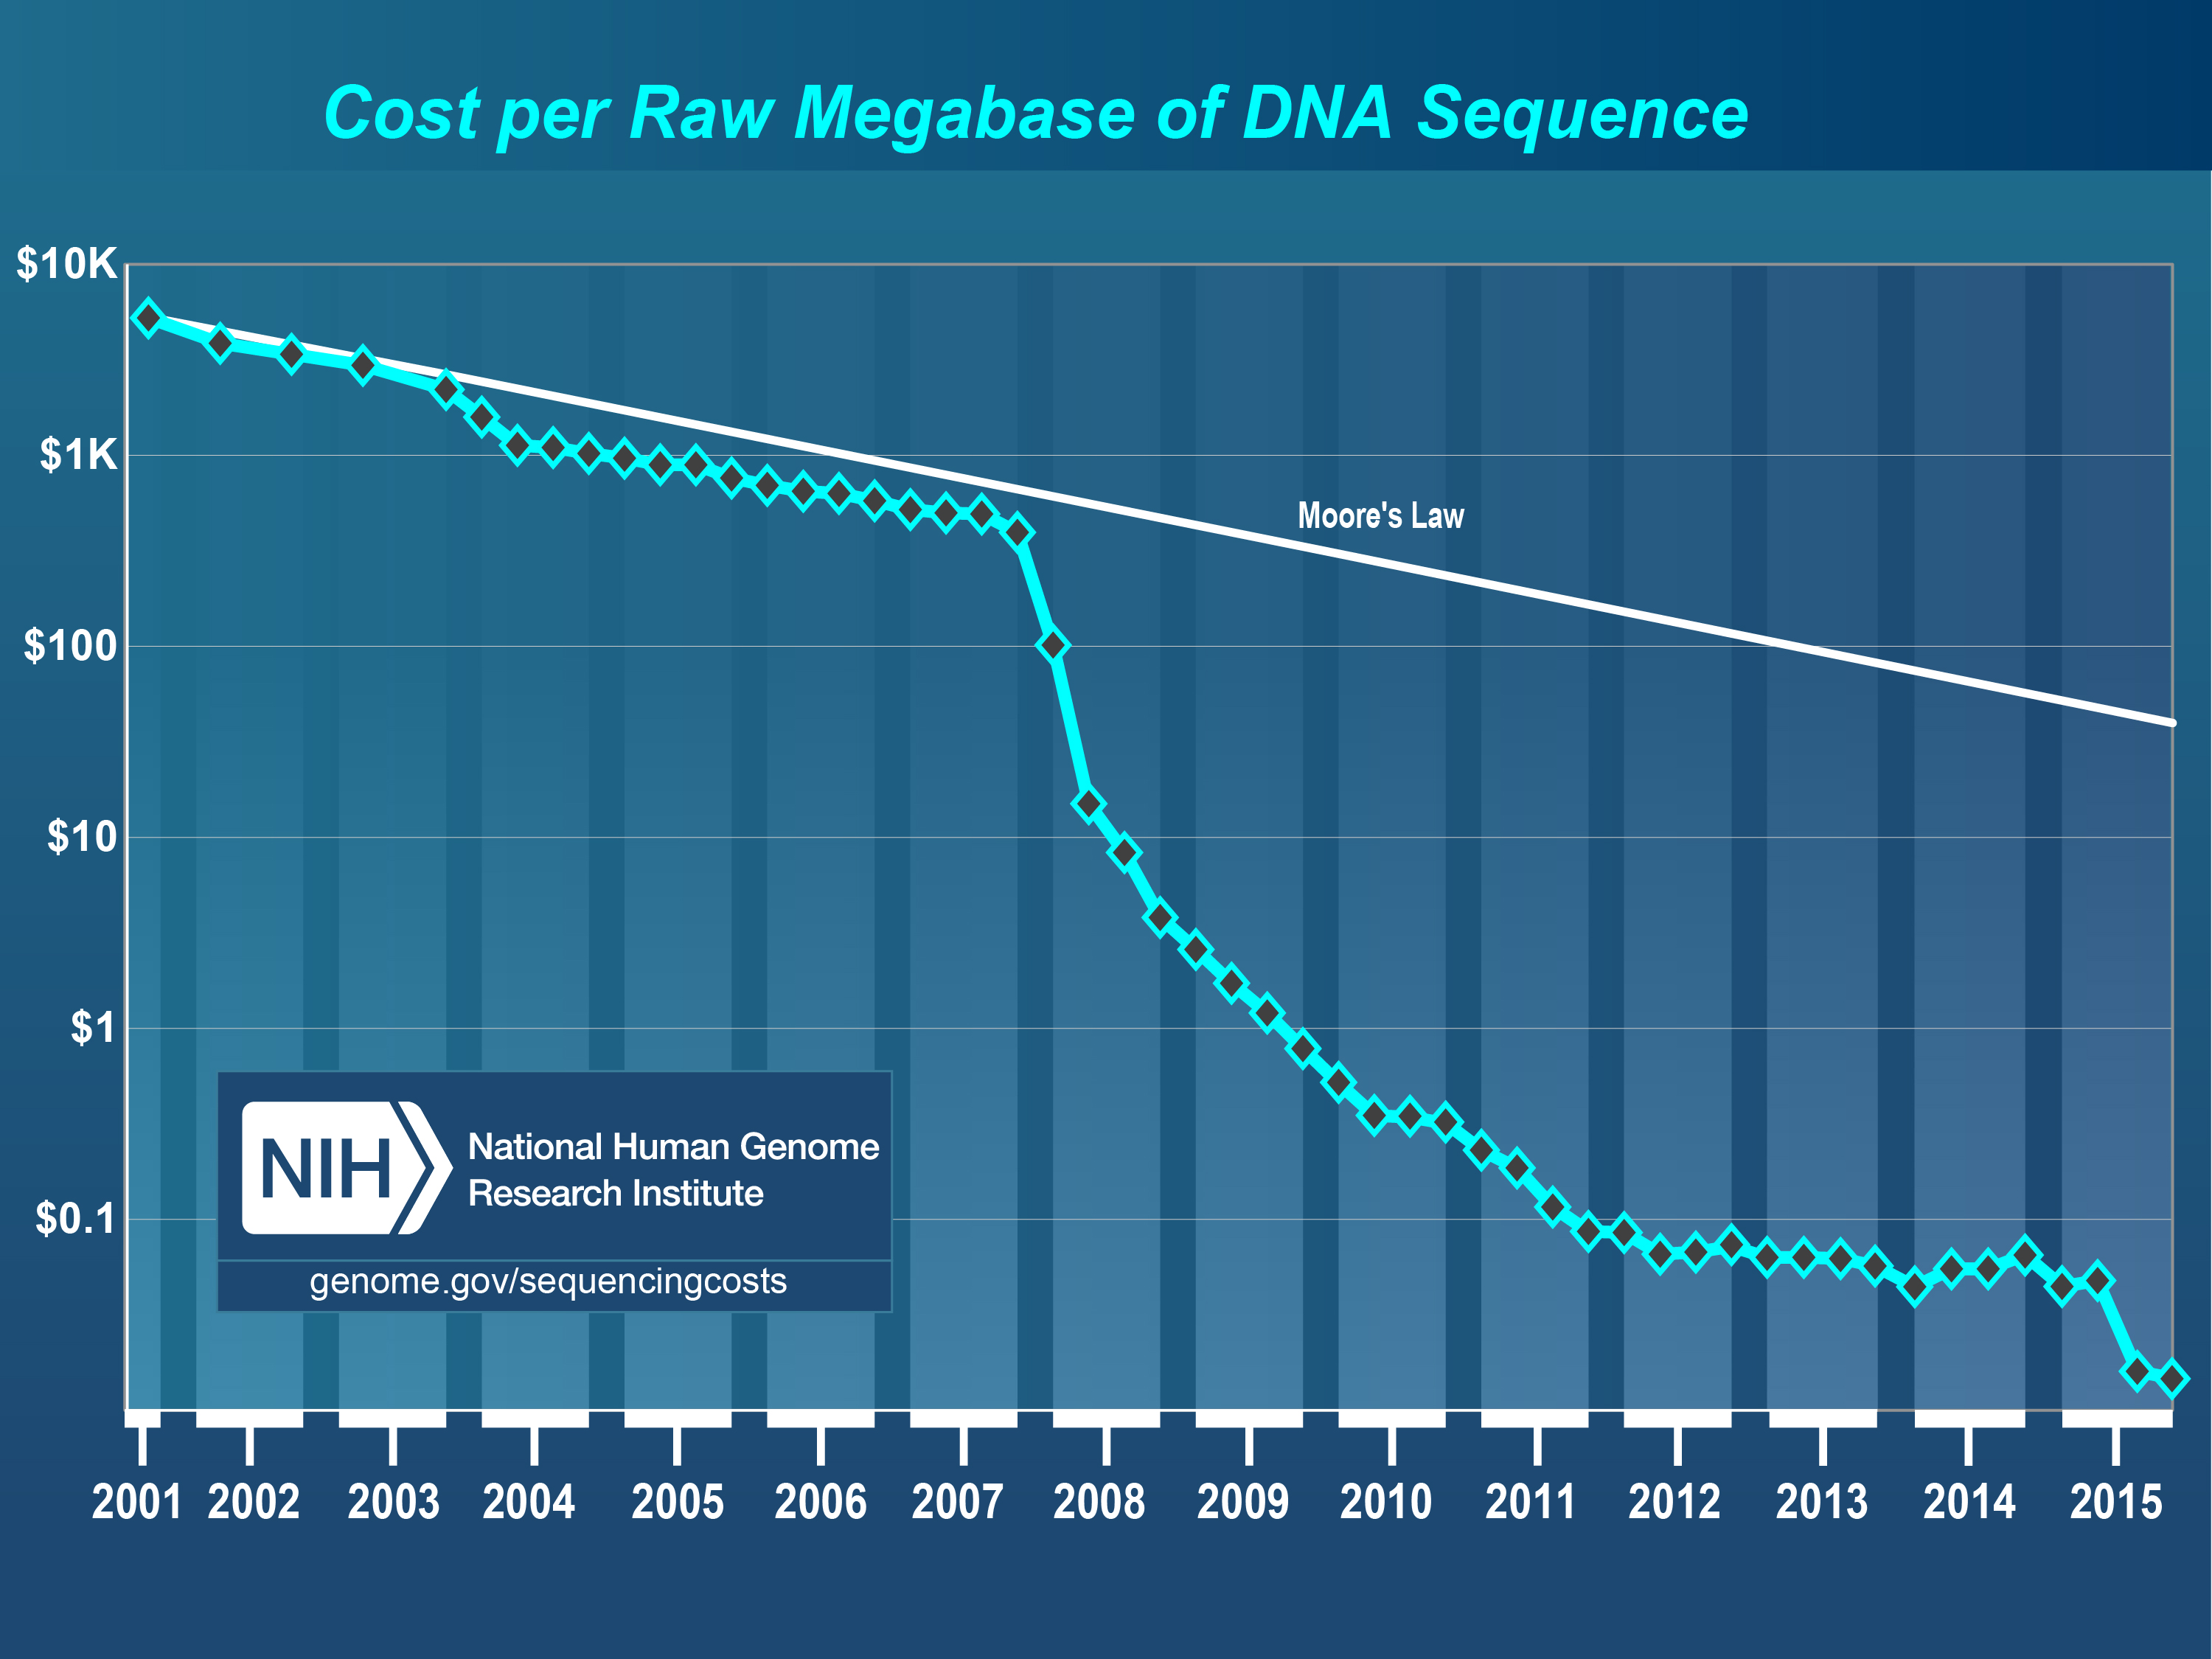
\includegraphics[scale=0.5]{costperMb2015_4.jpg}
\end{center}
\caption[Cost per raw megabase of DNA sequence from 2001 to 2015]{Cost per raw megabase of DNA sequence from 2001 to 2015. Straight line - Moore's Law, blue curve - cost in US dollars, Y-axis scale is logarithmic. Graph reproduced from \citep{wetterstrand2016}}
\end{figure}



\end{document}
